\documentclass[12pt, a4paper, reqno, oneside]{book}
\usepackage{amsmath,amsxtra,amssymb,latexsym, amscd,amsthm}
\usepackage{indentfirst}
\usepackage{color}
\usepackage[utf8]{vietnam}
\usepackage{amsmath}
\usepackage[mathscr]{eucal}
\usepackage{amsfonts}
\usepackage{graphics}
\usepackage[utf8]{inputenc}
\usepackage{amssymb}
\usepackage{calligra}
\usepackage{calrsfs}
%\input setbmp
\usepackage[unicode]{hyperref}
\usepackage{titledot}
\usepackage{graphicx}
\graphicspath{ {./images/} }
\titlename{Chương}
%+ Can le van ban
\setlength{\oddsidemargin}{0in}
\setlength{\textwidth}{6.in}
\setlength{\topmargin}{-0.5in}
\setlength{\textheight}{9.25in}
\renewcommand{\baselinestretch}{1.5}

%+ Dinh nghia mot so ky hieu toan hoc.
\def\B{\mathscr B}
\def\one{\mathbf 1}
\def\R{{\mathbb R}}
\def\LL{{\mathbb L}}
\newcommand\abs[1]{|#1|}
\newcommand\set[1]{\{#1\}}
\newcommand\norm[1]{||#1||}
\DeclareMathOperator{\vrai}{vrai}
\DeclareMathOperator{\const}{const}
\newcommand{\eoproof}{\hfill $\square$}
\newcommand{\spro}[1]{\left<#1\right>}
\newcommand{\argmin}{\arg\min}

\renewcommand{\theequation}{\arabic{chapter}.\arabic{section}.\arabic{equation}}
\theoremstyle{remark}
\newtheorem{lemma}{\bf Bổ đề}[section]
\newtheorem{theorem}{\bf Định lý}[section]
\newtheorem{proposition}{\bf Mệnh đề}[section]
\newtheorem{corollary}{\bf Hệ quả}[section]
\newtheorem{definition}{\bf Định nghĩa}[section]
\newtheorem{remark}{\bf Chú ý}[section]
\newtheorem{example}{\it Ví dụ}[chapter]

%+ Bat dau tai lieu tai day.
\begin{document}
%+ ====================================================
\makeatletter
\renewcommand{\ps@myheadings}{
\renewcommand{\@oddhead}{\textsf{Luận văn Thạc sỹ - ngành toán ứng dụng}\hfil\textrm{\thepage}}
\renewcommand{\@oddfoot}{\textsf{Nghiêm Minh Hoàng, CA160035, Toán ứng dụng.}\hfil}
}
\makeatother 

%+ Page style
\newpage
\input bialuanan

\pagestyle{plain}
\input loicamon

\tableofcontents
\newpage
\input loimodau

\newpage
%%%%%%%%%%%%%%%%%%%%%%%%%%%%%%%%%%%%%%%%%%%
%+ Chuong 1. Co so ly thuyet ma.
%+ Revised: 03-05-2008
%+ Last revised: 10-05-2008
%%%%%%%%%%%%%%%%%%%%%%%%%%%%%%%%%%%%%%%%%%%
\setcounter{chapter}{0}
\chapter{CƠ SỞ LÝ THUYẾT MÃ}

Trong chương này, chỉ những khái niệm cơ bản liên quan được sử dụng trong luận án mới được đề cập. Nội dung kiến thức về đại số, ngôn ngữ và mã của các từ hữu hạn trình bày trong các mục,
từ Mục \hyperlink{page.6}{\textcolor{blue}{1.1}} đến Mục \hyperlink{page.16}{\textcolor{blue}{1.4}}, được tham khảo và trích dẫn từ các tài liệu [\textcolor{red}{4; 5; 6; 7; 9; 13; 16; 18; 21; 27; 28}].. Bên cạnh đó, luân án còn giới thiệu một số lớp mã dựa trên các hình thức tích mới, hiệu quả của các lớp mã này trong các chương tiếp theo. Nội dung kiến thức về mã luân phiên và mã của các từ định biên trong trình bày trong Mục \textcolor{blue}{1.5} là một hướng nghiên cứu mới trong lý thuyết mã, được đề xuất gần đây trong các công trình [\textcolor{red}{14; 15; 23; 32; 33; 34; 35}]. Kiến thức về ngôn ngữ và mã của các từ vô hạn xem như một sự mở rộng các khái niệm trong lý thuyết mã truyền thống trường hợp vô hạn được tổng hợp từ các tài liệu [\textcolor{red}{3; 10; 11; 13; 19; 20; 24; 29; 31}], là nội dung của mục \textcolor{blue}{1.6}.
Trong luận án tập các số tự nhiên được ký hiệu là $\mathbb{N}$. Lực lượng của 1 tập hợp $X$ được ký hiện là Card($X$). Các bảng chữ đều được giả thiết là hữu hạn nếu không nói gì khác.
%*************************************************************************
%+ 1.1. Nua nhom va vi nhom
%************************************************************************
\section{Nửa nhóm và vị nhóm}

Ta nhắc lại rằng một nửa nhóm S là một tập hợp được trang bị một phép toán hai ngôi kết hợp, nếu không nói gì thêm ta sẽ ký hiệu theo lỗi nhân. Một nửa nhóm con (t.ư. nhóm con) T của S là một tập con 
của S cùng với phép toán cảm sinh là cho T trở thành nửa nhóm (t.ư. nhóm). Nửa nhóm S là một vị nhóm nếu S có đơn vị. Đơn vị của vị nhóm S là duy nhất và được ký hiệu là $1_S$.
Một vị nhóm con của vị nhóm S là một nửa nhóm con có chứa đơn vị của S.


\textit{Ví dụ 1.1.} $M = \{0,1\}$ là vị nhóm nhân với phần tử đơn vị là 1.

\textit{Ví dụ 1.2.}
    Với vị nhóm $M$ bất kỳ, ta trang bị cấu trúc vị nhóm cho tập tất cả các tập con $\mathcal{P}(M)$ của M bằng cách định nghĩa, với $X, Y \subset M$,
    $$
        XY = \{ xy | x \in X, y \in Y \}
    $$
    Phần tử đơn vị là $\{1\}$.
1.1 Nửa nhóm và vị nhóm
\textit{Ví dụ 1.3.} 
    Từ các vị nhóm $M, N$ ta có vị nhóm $M \times N$ là tích trực tiếp của $M$ và $N, M^{(n)}$ là tích trực tiếp của $n$ lần vị nhóm $M$.

    Cho các nửa nhóm (vị nhóm) $S$ và $T$. Ánh xạ $\varphi : S \rightarrow T$ được gọi là một {\it đồng cấu nửa nhóm} (t.ư. {\it vị nhóm}) nếu với mọi $a, b \in S$,
    $$
    \varphi(ab) = \varphi(a)\varphi(b)
    $$
    (t.ư $\varphi(ab) = \varphi(a)\varphi(b)$ và $\varphi(1_S) = 1_T$ với $1_S$ là đơn vị của $S$, $1_T$ là đơn vị của $T$).

    Đồng cấu $\varphi$ được gọi là {\it đơn cấu} (t.ư {\it toàn cấu, đẳng cấu}) nếu $\varphi$ là đơn ánh (t.ư. toàn ánh, song ánh). 
    Một đồng cấu từ vị nhóm $S$ vào chính nó thì được gọi là một {\it tự đồng cấu}.
    Một {\it tương đẳng} trên một vị nhóm $M$ là một quan hệ tương đương ${\theta}$ trên $M$ sao cho với mọi $m,m' \in M, u,v \in M$
    $$
    m \equiv m'mod\theta \Rightarrow umv \equiv um'vmod\theta 
    $$
    \hspace{10mm} Nếu $\varphi : M \to N$ là một đồng cấu vị nhóm thì {\it quan hệ} ({\it hạt nhân}) $\equiv_\varphi$ trên $\theta$, cho bởi $m \equiv_\varphi m'mod\theta {\Leftrightarrow}$ $\varphi(m) = \varphi(m')$ là một tương đẳng trên $M$. Ngược lại nếu $\theta$ là một tương đẳng trên vị nhóm $M$, tập thương $M/\theta$ với phép toán $[x]_\theta[y]_\theta = [xy]_\theta$, ở đó $[x]_\theta$ kí hiệu tương đương theo $\theta$ chưa $x$, là một {\it vị nhóm thương} của $M$ với tương đẳng $\theta$ và ta có {\it đồng cấu tự nhiên} $\theta^\aleph : M \to M/\theta$ cho bởi $\theta^\aleph(m) = [m]_\theta$ với mọi $m \in M$.\\
    Cho $M$ là một vị nhóm. Với $x, y \in M$, ta có: 
    \center{    
        $x^{-1}y = \{z \in M | x.z = y\} $ và $ xy^{-1} = \{z \in M | x= z.y \}.$
    }\\
    \begin{flushleft}
    \hspace{10mm} Với $S, T \subseteq M$, ta định nghĩa các phép cắt trái, phải của $S$ bởi $T$
    \end{flushleft}
    $
    T^{-1}S = \{u \in M \exists \in T : t.u \in S \}$ và $ST^{-1} = \{ u \in M \exists \in T : u.t \in S \}
    $
    \begin{flushleft}
    \hspace{10mm}Ta có tính chất cơ bản sau
    \end{flushleft}
\begin{flushleft}
    \textbf{Tính chất 1.1}  Cho $M$ là một vị nhóm , $P,K \subseteq M, P = K^*$ và $m \in M$. Khi đó $P^{-1}(m^{-1})K = (m.P)^{-1}K$.\\
    {\it Chứng minh.} Chứng minh $P^{-1}(m^{-1})K \subseteq (m.P)^{-1}K$. Ta có\\
    \hspace{10mm} $\omega \in P^{-1}(m^{-1})K \Leftrightarrow (\exists p \in P, k \in K : \omega = p^{-1}( m^{-1}k ) \Leftrightarrow k = m.p.\omega).$ \\
    Vi vậy $\omega = (m.p^{-1}k \in (m.P)^{-1}K.$ \\
    \hspace{10mm}Chứng minh $P^{-1}(m^{-1})K \subseteq P^{-1}( m^{-1}K )$. Ta có \\
    \hspace{20mm} $\omega \in ( m.P )^{-1}K \Leftrightarrow ( \exists p \in P , k \in K : \omega = ( m.p )^{-1}k \Leftrightarrow k = m.p.\omega ).$ \\
    Vì vậy $\omega = p^{-1}( m^{-1}k ) \in P^{-1}( m^{-1}K )$
\end{flushleft}
%+ Dinh nghia 1.1.1
\begin{definition}\label{de.1.1.1} 
Giả sử $C\subseteq R^n$ là một tập hợp khác rỗng.
\begin{itemize}
\item Tập $C$ gọi là tập lồi nếu với mọi $x,y\in C$ và mọi  $\lambda\in [0,1]$ ta có
$$\lambda x+(1-\lambda)y\in C$$

\item Giả sử $x^1,\dots, x^k$ là $k$ điểm của $C$ khi đó 
\begin{equation}\label{eq.1.1.1}
x  = \sum\limits_{i=1}^k\lambda_kx^k,\quad\text{với}\quad \lambda_k\geq 0,\sum\limits_{i=1}^k\lambda_k=1,\forall k =1,\ldots,k
\end{equation}
gọi là một tổ hợp lồi của hệ vector  $\{x^1,\ldots, x^k\}$.
\end{itemize}
\end{definition}
Cho $M\subseteq R^n$, ta nói bao lồi của một tập hợp $M$ là giao của tất cả các tập lồi chứa $M$, được kí hiệu là $\text{conv}(M)$. Rõ ràng bao lồi của $M$ là tập lồi nhỏ nhất chứa $M$. Một tập $C$ là lồi khi và chỉ khi nó chứa mọi tổ hợp lồi hữu hạn các điểm của $C$.

Một trong những tập lồi quan trọng (trong giải tích lồi, tối ưu (đặc biệt là quy hoạch tuyến tính)) là tập lồi đa diện. 
Tập lồi $P$ được gọi là tập lồi đa diện nếu $C$ có dạng
\begin{equation}\label{eq.1.1.2}
P := \{x\in R^n\; |\; Ax \leq b\}
\end{equation}
trong đó $A=(a_{ij})_{m\times n}, b\in R^m$. Hay nói cách khác, $P$ là giao của hữu hạn các nửa không gian đóng.
Trường hợp đặc biệt của tập lồi đa diện là đa diện chính tắc có dạng như sau:
\begin{equation}\label{eq.1.1.3}
P_0 := \set{x\in R^n\; |\; Ax = b, x\geq 0 }
\end{equation}
trong đó ma trận $A\in\R^{m\times n}, b\in\R^m$ và giả thiết $A$ có hạng đủ (tức là $\text{rank}A = m\leq n$).

%+ Dinh nghia 1.1.2.
\begin{definition}\label{de.1.1.2}\
\begin{itemize}
\item Tập $C$ được gọi là một nón nếu với mọi $x\in C$ và mọi $\lambda\geq 0$ ta có $\lambda x\in C$.
\item Tập $C$ được gọi là nón lồi nếu $C$ vừa là nón vừa là tập lồi.
\end{itemize}
\end{definition}
Bao nón lồi của tập $M$ là giao của tất cả các nón lồi chứa $M$, ký hiệu là $\text{conv}(M)$ và nó cũng là tập nón lồi nhỏ nhất chứa $C$. Nói $C$ gọi là nón lồi đa diện nếu $C$ vừa là nón vừa là tập lồi đa diện. Mỗi nón $C$ có một điểm $x=0$ gọi là gốc (mũi) của nón $C$. Tập $r:=\set{x\in C: x=x^0+\lambda d}$ gọi là một tia xuất phát từ $x^0$ theo hướng $d\neq 0$. Một nón $C$ sẽ chứa các tia xuất phát từ $x^0=0$.\\
Cho một tập lồi đa diện $P=\set{x\in\R^n\;:\; Ax=b}$ với $\text{rank} A=m\leq n$. Khi đó tập $K:=\set{d\;|\; Ad \geq 0}$ là một nón lồi đa diện, gọi là nón lồi sinh ra bởi các hướng cực biên của $P$ (như định nghĩa dưới đây). 

%+ Dinh nghia 1.1.2.
\begin{definition}\label{de.1.1.2}\
\begin{itemize}
\item Điểm $x^0$ là điểm cực biên (hai đỉnh) của tập lồi đa diện $P$ nếu nó không là điểm trong của bất kỳ đoạn nào nối hai điểm khác nhau của $P$, tức là $\nexists x', x'' \in P$ và $x' \neq x''$ sao cho 
$$
x^0 = \alpha x'+(1-\alpha)x''
$$
với $\alpha$ nào đó thuộc $(0,1)$.
\item Mỗi tập con $L$ của đa diện lồi $P$ gọi là một cạnh nếu với mọi $x,y\in P, \lambda\in (0,1)$ mà $\lambda x+(1-\lambda)y\in L$ thì $[x,y]\subseteq L$ và $L$ chứa trọn trong một đường thẳng. Một cạnh vô hạn gọi là một tia cực biên. Hướng của tia cực biên này gọi là hướng cực biên của $P$.
\end{itemize}
\end{definition}
Chú ý rằng, tập lồi đa diện đóng, bị chặn thì không có hướng cực biên. Số đỉnh và số hướng cực biên của tập lồi đa diện $P$ là hữu hạn.

%+ -------------------------------------------------------------------------------------------
%+ 1.1.2. Mot so dinh ly quan trong.
\begin{flushleft}
\subsection{Một số kết quả trong giải tích lồi}
\end{flushleft}
Phần này trình bày một số kết quả đã được đề cập trong giải tích lồi có liên quan đến khóa luận. Trước hết, cần nhắc lại một trong những định lý quan trọng là định lý biểu diễn tập lồi đa diện.
%+ Dinh ly 1.1.1. (Ve bieu dien tap loi da dien)
\begin{theorem}\label{th.1.1.1} 
Cho $P$ là tập lồi đa diện trong $\R^n$ với tập đỉnh là $V:=\set{v^i: i=1\dots,p}$ và tập các hướng cực biên là $E:=\set{d^j: j=1\dots q}$. Khi đó mọi điểm $x\in P$ đều có thể biểu diễn dưới dạng:
\begin{equation}\label{eq.1.1.2.1}
x = \sum_{i=1}^p\lambda_iv^i + \sum_{j=1}^q\gamma_jd^j,
\end{equation}
trong đó $\sum_{i=1}^p\lambda_i = 1, \lambda_i\geq 0, i=1,\dots,p$ và $\gamma_j\geq 0, j=1,\dots, q$.
\end{theorem}
Hiển nhiên nếu $P$ là đa diện lồi bị chặn thì biểu diễn chỉ còn lại
$$
x = \sum_{i=1}^p \lambda_iv^i.
$$
Một tập lồi đa diện khác rỗng, không chứa trọn một đường thẳng thì luôn có điểm cực biên và số điểm cực biên là hữu hạn. Để kiểm tra một điểm $x^0$ có là điểm cực biên của tập lồi đa diện, ta có định lý sau.

%+ Dinh ly 1.1.2. ( Xac dinh diem cuc bien (lam the nao kiem tra mot diem cua tap loi da dien P la diem cuc bien)).
\begin{theorem}\label{th.1.1.2}
Giả sử $P_0$ là một tập lồi đa diện chính tắc dạng
\begin{equation}\label{eq.1.1.2.2}
P_0 := \set{x\in R^n\; |\; Ax = b, x\geq 0 }
\end{equation}
trong đó ma trận $A\in\R^{m\times n}, b\in\R^m$ và giả thiết $A$ có hạng đủ (tức là $\text{rank}A = m\leq n$). Điểm $x^0$ là một điểm cực biên (đỉnh) của $P_0$ nếu và chỉ nếu tập các véc tơ cột $B:=\set{A_j: j\in J_+(x^0)}$ của ma trận $A$ là độc lập tuyến tính, trong đó
\begin{equation}\label{eq.1.1.2.3}
J_+(x^0):=\set{j\in\set{1,\dots, n}\;:\; x^0_j>0}.
\end{equation}
\end{theorem}

%%%%%%%%%%%
% 1.2 Từ và ngôn ngữ 
%%%%%%%%%%
\begin{flushleft}
    \section{Từ và ngôn ngữ}
\end{flushleft}
\begin{flushleft}
Cho $A$ là một \textit{bảng chữ} . Một từ $\omega$ trên bảng chữ $A$ là một dãy hữu hạn các phần tử của $A$
$$
    \omega = (a_1, a_2, a_3, ... , a_n), a_i \in A
$$
\hspace{10mm}Tập tất cả các từ trên bảng chữ $A$ được ký hiệu là $A^*$ và được trang bị phép nhân (tích) ghép có tính chất kết hợp 
$$
(a_1, a_2, ... , a_n)(b_1, b_2, ... , b_n) = (a_1, a_2, ... , a_n,b_1, b_2, ... , b_n).
$$
Vì vậy để thuận lợi ta viết 
$$
    \omega = a_1a_2...a_n
$$
thay cho $\omega = ( a_1, a_2, ... , a_n )$. Một phần tử $a \in A$ được gọi là một \textit{chữ cái. Từ rỗng} được ký hiệu là $\varepsilon$ đóng vai trò là phần tử đơn vị trong phép nhân ghép. Do đó, tập $A^*$ có cấu trúc vị nhóm và $A^*$ được gọi là vị nhóm tự do trên $A$. Tập tất cả các từ khác rỗng trên $A$ được ký hiệu là $A^+$ . Ta có $A^+$ . Ta có $A^+ = A^* - \{{\varepsilon}\}$ 
\hspace{10mm}Độ dài $|\omega|$ của từ $\omega = a_1a_2...a_n$ với $a_i \in A$ là $n.$ Quy ước $|\varepsilon|$ = 0. Ánh xạ $\omega \to |\omega|$ là một đồng cấu từ $A^*$ đến vị nhóm cộng $\mathbb{N}$. Với $n \ge 0$, ta ký hiệu 
$$
    A^{<n} = \{ \omega \in A | |\omega| \le n - 1 \}
$$
và 
$$
    A^{<n} = \{ \omega \in A | |\omega| \le n \}
$$
Đặc biệt $A^{<0} = \theta $ và $A^{<0} = \{ \varepsilon \}$. \\
\hspace{10mm}Một từ $\omega \in A^*$ là một \textit{khúc con} của một từ $ x \in A^*$ nếu tồn tại $u, v \in A^*$ sao cho $x = u\omega v$ Quan hệ \textit{"là một khúc con của"} là quan hệ thứ tự bộ phận trên $A^*$. Một khúc con $\omega$ của $x$ là \textit{khúc con thật sự} nếu $\omega \ne x$. Một từ $\omega \in A^*$ là một \textit{khúc đầu} (t.ư. \textit{khúc đuôi}) của một từ $\omega \in A^*$ nếu tồn tại một từ $u \in A^*$ sao cho $x = \omega u$ (t.ư. $x = u\omega$). Quan hệ \textit{"là một khúc con của"} (t.ư. \textit{"là một khúc đuôi của"} ) cũng là một quan hệ thứ tự bộ phận trên $A^*$. Ta viết $\omega \le_p x$ (t.ư. $\omega \le_s x$) khi $\omega$ là một khúc đầu (t.ư. khúc cuối) của $x$ và $\omega <_p x$ (t.ư. $\omega <_{s} x$ ) khi $\omega \le_{p}$ và $\omega \ne x$ ( t.ư $\omega \le_s x$ và $\omega \ne x$ ). Thứ tự này có tính chất cơ bản sau đây. Nếu có từ x,

\end{flushleft}
$\omega \le_p x, \omega' \le_p x, ($ t.ư $ \omega \le_s x, \omega' \le_s x ),$
\begin{flushleft}
thì $\omega$ và $\omega'$ so sánh được với nhau, tức là
\end{flushleft}
$\omega \le_p \omega'$ hoặc $\omega' \le_p \omega $ (t.ư $\omega \le_s \omega'$ hoặc $\omega' \le_s \omega $)
\begin{flushleft}
    1.2 Từ và ngôn ngữ\\
    \hspace{10mm} Tập con $X$ của $A^*$ được gọi là tập $prefix$ nếu không có từ nào của $X$ là khúc đầu thực sự của một từ khác trong $X$ .
    \hspace{10mm} Hai từ $x, y \in A^*$ được gọi là \textit{liên hợp} nếu tồn tại các từ $u, v$ sao cho $x = uv$, $y = vu$. Xem hình \hyperlink{page.12}{\textcolor{blue}{1.1}}. Khi đó ta cũng gọi $v$ là một $overlap$ của $x$ và $y$
    
\end{flushleft}
\begin{figure}[ht]
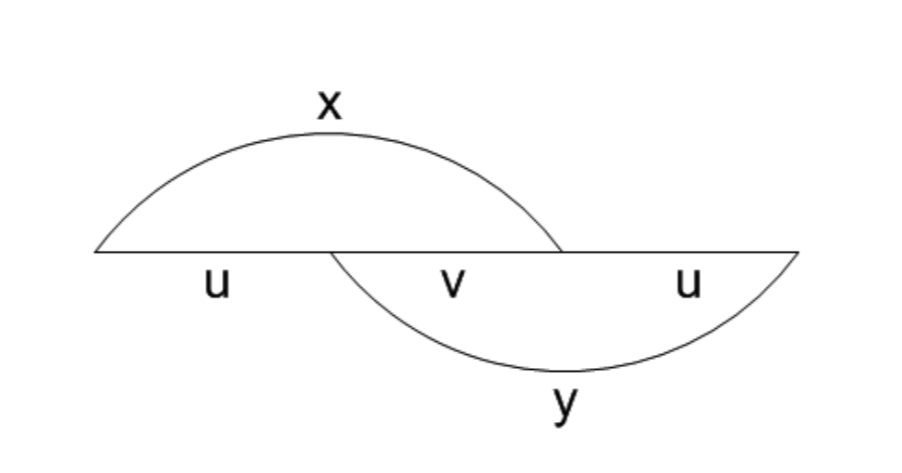
\includegraphics[scale=0.5]{1_1.png}
\caption{\textbf{Hình 1.1} \textit{Một overlap của hai từ liên hợp x và y}}
\end{figure}
\begin{flushleft}
Một tập con của $A^*$ được gọi là một \textit{ngôn ngữ} trên $A$.
Với một ngôn ngữ $X$ thuộc $A^*$, ta kí hiệp $X^*$ vị nhóm con sinh bởi $X$,
\end{flushleft}
$X^* = \{ x_1x_2...x_n | n \ge 0, x_i \in X\}$
\begin{flushleft}
Tương tự, ta kí hiệu $X^+$ nửa nhóm con sinh bởi $X$,
\end{flushleft}
$X^+ = \{ x_1x_2...x_n | n \ge 1, x_i \in X\}$
\begin{flushleft}
Ta có
\end{flushleft}
$$
\begin{cases}
    X^* - \{ \theta \} & \textit{nếu } \theta \not\in X, \\
    X^* & \textit{nếu } \theta \not\in X, \\
\end{cases}
$$
\begin{flushleft}
\hspace{10mm}Một \textit{phân tích} của một từ $\omega \in A^*$ theo các từ của $X$ cho bởi đẳng thức $\omega = x_1x_2...x_n, x_i \in X, i \ge 1$. Khi đó, ta cũng nói $\omega$ có một $X$-\textit{phân tích}. Theo định nghĩa, mỗi từ $\omega \in X^*$ có ít nhất một $X$-\textit{phân tích}. Để dễ hình dung, ta thường biểu diễn một $X$-\textit{phân tích} $\omega = x_1x_2...x_n, x_i \in X, i \ge 1$ bằng hình sau: \\
\end{flushleft}
\begin{figure}[ht]
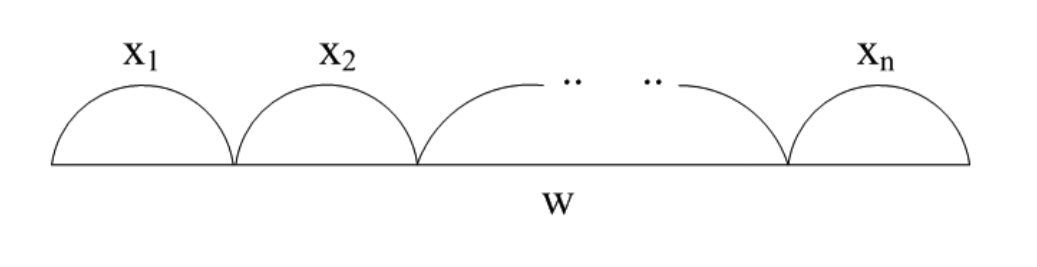
\includegraphics[scale=0.5]{1_2.png}
\caption{\textbf{Hình 1.2} \textit{Một X - phân tích từ} $\omega$}
\end{figure}
\begin{flushleft}
hspace{10mm}Cho $X, Y \subseteq A^*$ là các ngôn ngữ. \textit{Tích} của $X$ và $Y$, \textit{thương trái, thương phải} của $X$ bởi $Y$ là các ngôn ngữ được định nghĩa ở mục trước với vị nhóm $M = A^*$. với $\omega, v \in M$, ta sẽ viết $uv$ thay cho $u.v$. Khi đó:
\end{flushleft}
$XY = \{ xy|x \in X , y \in Y\}$,\\
$Y^{-1}X = \{ \omega \in A^* | y\omega \in X , y \in Y\}$,\\
$XY^{-1} = \{ \omega \in A^* | y\omega \in X , y \in Y\}$
\begin{flushleft}
Ký hiêu $u^{-1}X, Xu^{-1}$ được sử dụng khi tập $Y$ chỉ có một phần tử $Y = \{ u \}$.
\end{flushleft}
%*************************************************************************
%+ 1.3. Otomat và ngôn ngữ chính quy 
%**********************************************************
\begin{flushleft}
\section{Otomat và ngôn ngữ chính quy}
Cho A là một bảng chữ, một \textit{otomat} trên A là một bộ $\mathcal{A}$ = $(\mathcal{Q},A, \mathcal{F})$ gồm một tập hữu hạn các trạng thái Q và các tập $\mathcal{F} \subseteq Q \times A \times Q$, mỗi cung có dạng \textit{p,a,q} với \textit{p} là đỉnh đầu, $q$ là đỉnh cuối và $a$ là nhãn của cung. Ta còn biểu diễn một Otomat với \textit{tập trạng thái khởi đầu} $I \subseteq Q$ và \textit{tập trạng thái kết thúc} $T \subseteq Q$ bởi $( Q, A, \mathcal{F}, I, T )$ hoặc ngắn gọn $(Q, I, T)$ khi $A$ và $\mathcal{F}$ cố định.
\end{flushleft}
\hspace{10mm}Otomat $\mathcal{A}$ = $(Q, A, \mathcal{F})$ là \textit{hữu hạn} nếu tập trạng thái $Q$ hữu hạn.\\
\hspace{10mm}Một \textit{đường đi} trong otomat $A$ là một dãy $c$ = $(f_1, f_2, ... ,f_n)$ các cung liền nhau \\
$f_i$ = $(q_i, a_i, q_{i+1})$,  $1 \le i \le n.$
\begin{flushleft}
    \hspace{10mm}Số $n$ được gọi là \textit{độ dài} của đường đi $c$. Từ $w$ = $a_1a_2...a_n$ là \textit{nhãn} của đường đi $c$. Trạng thái $q_1$ là \textit{điểm đầu} và trạng thái $q_{n+1}$ là \textit{điểm cuối} của $c$. Để thuận tiện khi tham chiếu đến đường đi $c$, ta sử dụng ký hiệu
\end{flushleft}
$c$ : $q_1$ $\xrightarrow{w} q_{n+1}.$
\begin{flushleft}
    Quy ước, với mỗi trạng thái $q \in Q$ , có một đường đi độ dài 0, nhãn $\varepsilon$, từ $q$ đến $q$. 
\end{flushleft}
\begin{flushleft}
\hspace{10mm}Một đường đi $c : i \to t$ là \textit{đường đi thành công} nếu $i \in I$ và $t \in T$. Ngôn ngữ \textit{đoán nhận được} bởi $\mathcal{A}$ ký hiệu là $L(\mathcal{A})$, được định nghĩa là tập các nhãn của các đường đi thành công. $L(\mathcal{A})$ = $\{ w \in A^* $ | $ \exists c : i \xrightarrow{w} t, i \in I, t\in T \}$.
\end{flushleft}
\begin{flushleft}
\hspace{10mm}Một Otomat $\mathcal{A}$ = $(Q, I, T)$ là \textit{đơn định} nếu $Card(I)=1$ và nếu  
\end{flushleft}
$(p,a,q),(p,a,r) \in \mathcal{F} \Rightarrow q = r$.
\begin{flushleft}
\hspace{10mm}Vì vậy, với mỗi $P \in Q$ và $a \in A$ có nhiều nhất một trạng thái $q \in Q$ sao cho $p \xrightarrow{a} q$. Với $p \in Q$ và $a \in A$, ta định nghia 
\end{flushleft}
$p.a$ = $\begin{cases}
    q \text{  nếu  } (p,a,q ) \in \mathcal{F},\\
    \emptyset \text{  nếu  } (p,a,q) \not\in \mathcal{F}.\\ 
\end{cases}$
\begin{flushleft}
    Hàm bộ phận
\end{flushleft}
$Q \times A \to Q$
\begin{flushleft}
định nghĩa như trên được mở rộng cho từ bằng cách đặt, với mọi $q \in Q$,
\end{flushleft}
$p.\varepsilon$ = $P$,
\begin{flushleft}
và, với $w \in A^*$ và $a \in A$, 
\end{flushleft}
$p.wa$ = $(p.w).a$
\begin{flushleft}
Hàm định nghĩa như trên được gọi là \textit{hàm chuyển} của $\mathcal{A}$. Khi đó, với $I$ = $\{ i \}$ ta có
\end{flushleft}
$L(\mathcal{A})$ = $\{ w \in A^* \text{ | } i.w \in T \}$.
\begin{flushleft}
\hspace{10mm}Cho $X \subseteq A^*$ là một ngôn ngữ chính quy. Ta định nghĩa một otomat hữu hạn đặc biệt $\mathcal{A}(X)$ = $(Q, i, T)$ như sau. Các trạng thái của $\mathcal{A(X)}$ là các tập khác rỗng 
\end{flushleft}
$u^{-1}X$
\begin{flushleft}
Với $u \in A^*$. Trạng thái khởi đầu là $X$ = $\varepsilon^{-1} X$, và các trạng thái kết thúc có chứa từ rỗng. Hàm chuyển cho một trạng thái $Y$ = $u^{-1} X$ và một chữ cái $a \in A$ được cho bởi  
\end{flushleft}
$Y \xrightarrow{a} a^{-1} Y$.
\begin{flushleft}
Đây là một hàm bộ phận và ta có 
\end{flushleft}
$L(\mathcal{A(X)})$ = X.
\begin{flushleft}
\hspace{10mm}Ta biết rằng theo \hyperlink{page.78}{\textcolor{red}{5}}, otomat $\mathcal{A} (X)$ được gọi là \textit{otomat tối tiểu} của X theo nghĩa đơn định, có số trạng thái ít nhất mà đoán nhận X. 
\end{flushleft}
\begin{flushleft}
\hspace{10mm}Cho $\mathcal{A}$ = $(Q, i, T)$ là một Otomat đơn định. Ta xét tập $\mathcal{F}$ của các hàm bộ phận từ $Q$ đến Q. Các hàm này được viết về phía bên phải: nếu $q \in Q$ và $m \in \mathcal{F}$ khi đó ảnh của $q$ bởi $m$ được ký hiệu là $qm$. Hàm hợp được định nghĩa bởi 
\end{flushleft}
$q (mn) = (qm) n $
\begin{flushleft}
\hspace{10mm}Vì vậy $\mathcal{F}$ có cấu trúc vị nhóm 
\end{flushleft}
\begin{flushleft}
\hspace{10mm}Xét $\varphi$ là một ánh xạ cho tương ứng mỗi từ $w \in A^*$ một hàm bộ phận từ $Q$ đến $Q$ định nghĩa bởi 
\end{flushleft}
$q \varphi (w) $ = $q.w.$
\begin{flushleft}
    \hspace{10mm}Khi đó, ánh xạ $\varphi$ là một đồng cấu từ $A^*$ đến vị nhóm $\mathcal{F}$, và vị nhóm $\varphi (A^*) $ của $\mathcal{F}$ được gọi là \textit{vị nhóm các phép chuyển dịch} của otomat $\mathcal{A}$.\\
    \hspace{10mm}Một đồng cấu $\varphi$ từ $A^*$ đến một vị nhóm $M$ được gọi là thoả mãn ngôn ngữ $X \subseteq A^*$ nếu tồn tại $B \subseteq M$, $B$ = $\varphi(X)$ sao cho 
\end{flushleft}
$\varphi^{-1}(B)$ = $X$.
\begin{flushleft}
    \hspace{10mm}Khi đó, ta cũng nói $X$ \textit{thoả bởi} $M$ và $X$ cho bởi một bộ ba $(\varphi, M, B)$.
    \hspace{10mm}Cho $X, Y \subseteq A^*$ là các ngôn ngữ. Ta thiết lập bổ đề kỹ thuật sau đây về tính thoả được làm cơ sở xây dựng các thuật toán trên vị nhóm trong các chương trình tiếp theo.
\end{flushleft}
\begin{flushleft}
\textbf{Bổ đề 1.1} \hspace{10mm} \textit{Giả sử h:} $A^* \to M$ \textit{là một toàn cấu vị nhóm thoả X và Y và gỉa sử} $X$ = $h^{-1}(K)$, $Y$ = $h^{-1}(L)$, $h(X^+)$ = $T$ \textit{với} $K, L, T \subseteq M$. Khi đó
\end{flushleft}
$X \cup Y$ = $h^{-1}(L \cup L)$, $X \cap Y$ = $h^{-1}(K \cap L)$, $X - Y$ = $h^{-1}(K - L)$,\\
$X^{-1}Y$ = $h^{-1}(K^{-1}L)$, $XY^{-1}$ = $h^{-1}(KL^{-1})$, $(X^+)^{-1}Y$ = $h^{-1}T^{-1}L$,\\
$Y(X^+)^{-1}$ = $h^{-1}(LT^{-1})$.
\begin{flushleft}
\textit{Chứng minh}. Giả sử $X$ = $h^{-1}(K)$, $Y$ = $h^{-1}(L)$, $K, L, \subseteq P$, ta chứng mình $X \cup Y$ = $h^{-1}(K \cup L)$. \\
\hspace{10mm}Trước hết, ta chứng minh $X \cup Y \subseteq h^{-1}(K \cup L)$. Thật vậy, với mọi $w \in X \cup Y$, ta có $h(w) \in K$ hoặc $h(w) \in L$. Vậy $X \cup Y \subseteq h^{-1}(K \cup L)$. \\
\hspace{10mm}Ngược lại, ta chứng minh $h^{-1}(K \cup L) \subseteq X \cup Y$. Thật vâtj, với mọi $w \in h^{-1}(K \cup L)$, ta có $h(w) \in K \cup L$. Nghĩa là $w \in X \cup Y$. Vậy $h^{-1}(K \cup L) \subseteq X \cup Y$. \\
\hspace{10mm}Ta chứng minh tương tự cho các quan hệ $X \cap Y$ = $h^{-1}(K \cap L)$, $X - Y$ = $h^{-1}(K - L)$, $X^{-1}Y = h^{-1}(K - L)$, $X^{-1}Y$ = $h^{-1}(K^{-1}L)$ và $XY^{-1}$ = $h^{-1}(KL^{-1})$. \\
\hspace{10mm}Từ giả thiết $h(X^+)$ =$T$ và $X = h^{-1}(K)$ ta có $K^+$ = $T$. Để chứng minh $(X^+)^{-1}Y$ = $h^{-1}(T^{-1}L)$, ta chứng minh $(X^+)^{-1}Y \subseteq h^{-1}(T^{-1}L) \subseteq (X^+)^{-1}Y$.
\hspace{10mm}Trước hết, ta chứng minh $(X^+)^{-1}Y$ = $h^{-1}(T^{-1}L)$. Thật vậy, với mọi $w \in (X^+)^{-1}Y$, tồn tại $x_1, x_2, ..., x_n \in X, y \in Y$ sao cho $x_1x_2...x_nw = y$. Từ đó suy ra $h(x_1).h(x_2)...h(x_n) = h(y) \in L$. Hơn nữa, từ $h(x_i) \in K$ suy ra $h(w) \in (K^+)^{-1}L$. Vậy $w \in h^{-1}(T^{-1}L)$. \\
\end{flushleft}
Ngược lại ta chứng minh $h^{-1}(T^{-1}L) \subseteq (X^+)^{-1}$. Đặt $w \in h^{-1}(T^{-1}L)$, ta có \\
$h(w) \in T^{-1}L$ = $(K^+)^{-1}L \Leftrightarrow \exists \alpha \in K^+ : \alpha.h(w) \in L$. 
\begin{flushleft}
Từ $\alpha \in K^+$ suy ra $\alpha$ = $\alpha_1\alpha_2...\alpha_p, \alpha_i \in K, i = 1,...,o$. Từ giả thiết h là toàn cấu và $X = h^{-1}(K)$ suy ra tồn tại $x_i \in X, i = 1,...,p$ sao cho $\alpha_i$ = $h(x_i)$. Ta có $\alpha = h(x1x_2...x_p)$, khi đó $\alpha.h(w)$ = $h(x_1x_2...x_pw)$. Từ đó suy ra $x_1x_2...x_pw \in h^{-1}(L)$ = $Y$ và ta có $ư \in (X^+)^{-1}Y$. \\
\hspace{10mm}Chứng minh $Y(X^+)^{-1}$ = $h^{-1}(LT^{-1})$ tương tự.\\
Vậy chứng minh được hoàn thành.\\
\hspace{10mm}Cho $X \subseteq A^*$ là một ngôn ngữ. Với $w \in A^*$, ta định nghĩa \textit{tập ngữ cảnh}
\end{flushleft}
Context($w$) = $\{ (u,v) \in A^* \times A^* | uwv \in X \}$.
\begin{flushleft}
\hspace{10mm}\textit{Tương đẳng cú pháp} của $X$ là một quan hệ tương đương $\equiv_X$ trên $A^*$ được định nghĩa bởi 
\end{flushleft}
$w \equiv_x w' \Leftrightarrow Context(w) = Context(w')$.
\begin{flushleft}
\hspace{10mm}Tập thương của $A^*/ \equiv_x được gọi là$ \textit{Vị nhóm cú pháp} của $X$. Ta ký hiệu vị nhóm cú pháp của $X$ là $M_x$ và kí hiệu $\varphi_x$ là đồng cấu chính tắc từ $A^*$ đến $M_x$, gọi là \textit{đồng cấu cú pháp} của X.\\
\hspace{10mm}Cho $X \subseteq A^*$ là một ngôn ngữ, ta có các kết quả sau đây về tính thoả thuận theo $\varphi_x$, mối liên hệ giữa vị nhóm cú pháp của $X$ và otomat tối tiểu của $\mathcal{A}(X)$ \\
\textbf{Mệnh đề 1.1} (\hyperlink{page.80}{\textcolor{red}{5}})  Cho $X \subseteq A^*$ \textit{là một ngôn ngữ và cho} $\varphi : A^* \to M$ \textit{là một toàn cấu vị nhóm. Nếu $\varphi$ thoả mãn X thì tồn tại một đồng cấu $\psi$ từ M đến vị nhóm cú pháp $M_x$ sao cho $\varphi_x = \psi \circ \varphi$}. \\
\textbf{Mệnh đề 1.2} (\hyperlink{page.80}{\textcolor{red}{5}})  Cho $X \subseteq A^*$ \textit{là một ngôn ngữ. Vị nhóm cú pháp của X đẳng cấu với vị nhóm các phép chuyển dịch của otomat tối tiểu $\mathcal{A}(X)$}.\\
\hspace{10mm}Lớp các \textit{ngôn ngữ chính quy} trên $A^*$(trên $A^+$) được ký hiệu là $RecA^*(RecA^+)$. Ta biết rằng $RecA^*$ là lớp các ngôn ngữ sinh bởi các ngôn ngữ {$a$}, với $a$ là một chữ cái thuộc A, các phép toán Boole($\cup, \cap, - $), phép nhân và phép lặp *, và cũng là lớp các ngôn ngữ đoán nhận được bởi otomat hữu hạn, $RecA^+$ = $\{ L \in RecA^* | L \subseteq A^+ \}$. \\
Ta có\\
\textbf{Mệnh đề 1.3} (\hyperlink{page.80}{\textcolor{red}{5}})  \textit{Lớp các ngôn ngữ chính quy trên $A^*$ đóng đối với phép toán Boole: phép hợp ($\cup$), phép giao ($\cap$), phép lấy phần bù ($-$)}.\\
\hspace{10mm}Định lý sau đây đặc trưng các tính chất của otomat hữu hạn \\
\textbf{Định lý 1.1} (\hyperlink{page.80}{\textcolor{red}{5}})  Cho $X \subseteq A^*$ \textit{là một ngôn ngữ. Các mệnh đề sau đây tương đương}\\
\hspace{10mm}\textit{(i)    X là chính quy}.\\
\hspace{10mm}\textit{(ii)    X là đoán nhận bởi một otomat hữu hạn (hoặc X là đoán nhận được)}.\\
\hspace{10mm}\textit{(iii)    Otomat tối tiểu $\mathcal{A}(X)$ là hữu hạn}.\\
\hspace{10mm}\textit{(i$v$)    Họ các tập}.\\
\end{flushleft}
$u^-1X$,
\begin{flushleft}
\hspace{20mm} với $u \in A^*$, là hữu hạn.\\
\hspace{10mm}\textit{($v$)    Vị nhóm cú phép $M_x$ là hữu hạn}.\\
\hspace{10mm}\textit{($vi$)   X thoả bởi một đồng cấu từ $A^*$ đến một vị nhóm hữu hạn M}.\\
\textit{Nhận xét 1.1}   Giả sử $X \subseteq A^+ $thoả bởi một đồng cấu vị nhóm $\varphi : A^* \to M$ từ $A^*$ đến một vị nhóm hữu hạn M. Nếu X là ngôn ngữ chính quy, ta có thể chọn M là vị nhóm các phép chuyển dịch của otomat tối tiểu đoán nhận X, hoặc vị nhóm cú pháp $M_x$ hữu hạn của X. Ta gọi $m = Card(M_x)$ \textit{là chỉ số tương đẳng cú pháp} của X, hay đơn giản, \textit{m là chỉ số} của X, hoặc X có chỉ số $m$.\\
\hspace{10mm}Từ bổ đề \hyperlink{page.17}{\textcolor{blue}{1.1}} và Mệnh đề \hyperlink{page.17}{\textcolor{blue}{1.3}}, ta có \\
\textbf{Hệ quả 1.1} Cho $X, Y \subseteq A^*$ \textit{là các ngôn ngữ chính quy, P là một vị nhóm hữu hạn và $h : A^* \to P$ là một toàn cấu vị nhóm. Nếu $X$ và $Y$ cùng thoả bởi h, thì h thoả tất cả các ngôn ngữ $L \in \mathcal{A}(X, Y)$, với $\mathcal{A}(X, Y)$ là tập tất cả các ngôn ngữ sinh ra bởi X, Y nhờ thực hiện một số hữu hạn các phép toán hợp, giao, lấy phần bù, lấy thương trái và lấy thương phải.}\\
\hspace{10mm} Mệnh đề sau đây được suy từ định nghĩa cho phép ta xây dựng toàn cấu $h$ trong hệ quả trên.\\
\textbf{Mệnh đề 1.4}    \textit{Cho $X, Y \subseteq A^*$ là các ngôn ngữ chính quy $, f : A^* \to M và g : A^* \to N $ là các đồng cấu vị nhóm, f thoả X và g thoả Y. Giả sử $h : A^* \to P \subseteq M \times N$ là một toàn cấu vị nhóm cho bởi: $\forall \in A^*, h(a) = (f(a),g(a)$ và P là một vị nhóm con của $M \times N$ sinh bởi tập tất cả các phần tử $h(a), a \in A$. Khi đó h thoả đồng thời X và Y}.\\
\begin{flushleft}
\textit{Ví dụ 1.4}  Cho $\varphi : A^* \to M$ là một đồng cấu vị nhóm thoả $X, Y \subseteq A^*, A \ne \emptyset$ và cho $Y = \{ \varepsilon \}$. Ta xây dựng toàn cấu $h$ thoả cả X và Y theo một trong 2 cách sau.\\
\hspace{10mm}Cách 1. Cho $Z_2 = \{ 0,1 \}$ là vị nhóm nhân modulo 2 của các số nguyên với đơn vị 1. Rỡ tàng, $Y = \{ \varepsilon \}$ thoả bởi đồng cấu $y : A^* \to Z_2$, được định nghĩa bởi $g(\varepsilon) = 1$ và với mọi $a \in A, g(a) = 0$. Ta có thể kiểm tra X và Y = {$\varepsilon$} cùng thoả bởi toàn cấu vị nhóm\\
$h : A^* \to P \subseteq M \times Z_2$ được cho bởi $\forall a \in A, h(a)$ = $(\varphi (a) , 0), 1_p$ = $h(\varepsilon)$ = $(1_M, 1)$.\\
Đặt $\overline{K}$ = $h(A) \cup 1_P$ = $\{ (h(a), 0) | a \in A \cup 1_P \}$, tâ có $\overline{A}^*$ = $P$.
\hspace{10mm}Cách 2. Mở rộng vị nhóm $M$ thành vị nhóm $M^1$ = $M \cup \{1\}$ với $1 \not\in M$ là phần tử đơn vị mới của $M^1$ bởi điều kiện ($\textbf{1}.x = x.\textbf{1} = x, \forall x \in M^1$).
\hspace{10mm}Định nghĩa $h' : A^* \to M^1$ ta định nghĩa toàn cấu $h : A^* \to P$ = $h'(A)^* \subseteq M^1$ cho bởi $h' : h(a)$ = $h'(a), \forall a \in A, h(\varepsilon) = h'(\varepsilon) = 1$.
\section{Mã của các từ hữu hạn}
\subsection{Mã và các tính chất đại số của mã}
Trong phần này ta xem xét định nghĩa và một số tính chất quan trọng của mã. Trước hết ta nhắc lại khái niệm tích không nhập nhằng là cơ sở để xây dựng khái niệm mã.\\
\hspace{10mm}Cho A là một bảng chữ và $X, Y \subseteq A^*$ là các ngôn ngữ. Tích $XY$ là \textit{không nhập nhằng} nếu mỗi từ $w \in XY$ có duy nhất một phân tích $w = xy$ với $x \in X, y ư\in Y$.\\
\textbf{Định nghĩa 1.1}     \textit{Giả sử A là một bảng chữ hữu hạn. Tập $X \subseteq A^+ $ là mã trên A nếu với mọi $n,m \ge 1$ và với mọi $x_1x_2,...,x_n,y_1y_2,...,y_m \in X$, nếu có} 
\end{flushleft}
\end{flushleft}
$x_1x_2...x_n$ = $y_1y_2...y_m$
\begin{flushleft}
\textit{thì khi đó}
\end{flushleft}
$n = m$ và  $x_i = y_i$     với     $i = 1,...,n$.
\begin{flushleft}
Cho $X \subseteq A^*$ là một ngôn ngữ. Từ định nghĩa của mã ta suy ra các tính chất sau đây.\\
\textbf{Tính chất 1.2}      X là mã nếu mỗi từ $x \ A^*$ (t.ư $w \in X^*$) có nhiều nhất (t.ư chỉ có duy nhất) một $X$-phân tích.\\
\textbf{Tính chất 1.3}    X là mã khi và chỉ khi $X^{-1}X \cap X^*(X^*)^{-1}$ = $\{ \varepsilon \}$.
\textit{Ví dụ 1.5}  Ngôn ngữ $X = \{ ab,abb,bb \}$ trên bảng chữ $A = \{ a,b \}$ là mã. Thật vậy, giả sử X không là mã. Khi đó tồn tại một từ $w \in X^+$ có độ dài tối tiểu thừa nhập hai X-phân tích khác nhau.
\end{flushleft}
$w = x_1x_2...x_n = y_1y_2...y_m$ với $x_1 \ne y_1$
\begin{flushleft}
$(n, m \le 1, x_i, y_i \in X )$. Từ đó $x_1 \ne y_1$ suy ra $x_1$ là khúc đầu của $y_1$ hoặc ngược lại. Giả sử $x_1$ là khúc đầu của $y_1$. Với $X$ như trên, ta có $x_1 = ab$ và $y_1 = abb$. Từ đó suy ra $x_2 = bb, y_2 = bb$. Vậy $y_1 = x_1b, y_1y_2 = x_1x_2b$. Thực hiện chứng minh quy nạp theo $k \le 1,$ ta có $x_{k+1} = bb$ và $y_{k+1} = bb$. Từ đó suy ra $y_1y_2...y_{k+1}$ = $x_1x_2...x_{k+1}b$ với mọi $k \le 1$. Điều này có nghĩa là không thể có từ $w$ hữu hạn thừa nhận hai X-phân tích khác nhau, trái với giả thiết. \\
\begin{figure}[ht]
    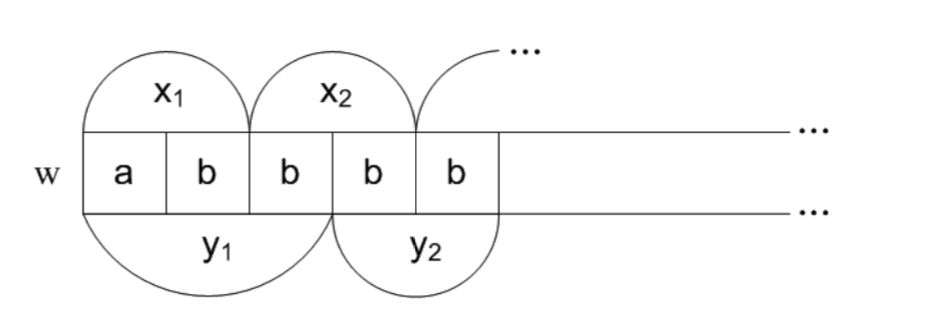
\includegraphics[scale=0.5]{1_3.png}
    \caption{ \textit{Khởi đầu một phân tích kép của từ $w$} }
\end{figure}
\textit{Ví dụ 1.6}  Cho $A = \{ a.b \}$ và $X = \{ b, abb, abbba, bbba, baabb \}$. Ngôn ngữ X không là mã vì tồn tại $w = abbbabbbaabb, w$ có hai X-phân tích khác nhau,
\end{flushleft}
$w = (abbba)(bbba(abb)$ = $(abb)(b)(abb)(baabb)$.\\
Định nghĩa mã theo cách sau đây cho phép ta diễn tả ý nghĩa của thuật ngữ \textit{mã}.
\begin{flushleft}
\textbf{Mệnh đề 1.5} (\hyperlink{page.80}{\textcolor{red}{5}})  \textit{Nếu $X \subset A^*$ là mã thì mỗi đồng cấu $\beta$ : $B^* \to A^*$ cảm sinh một song ánh từ bảng chữ B đến X là đơn cấu. Ngược lại, nếu tồn tại đơn cấu $\beta : B^* \to A^*$ sao cho X = $\beta(B)$, thì X là mã.}
\hspace{10mm}Một đơn cấu $\beta : B^* \to A^*$ với $X = \beta(B)$ được gọi là một \textit{đồng cấu mã} đối với X. Mệnh đề \hyperlink{page.20}{\textcolor{blue}{1.5}} trình bày ý nghĩa gốc củ thuật ngữ \textit{mã} vì các từ của X mã hoá các chữ cái của bảng chữ B. Thủ tục mã kết hợp một \textit{từ bản rõ} $b_1b_2...b_n (b_i \in B)$ với một \textit{từ mã} $\beta(b_1)...\beta(b_n)$ bởi sử dụng đồng cấu mã $\beta$. Sự kiện $\beta$ là đơn cấu đảm bảo từ mã được giải mã theo một cách duy nhất thành từ bản rõ ban đầu.\\
\hspace{10mm} Từ mệnh đề \hyperlink{page.20}{\textcolor{blue}{1.5}} ta có \\
\textbf{Hệ quả 1.2} (\hyperlink{page.81}{\textcolor{red}{5}})  \textit{ Giả sử $\alpha : A^* \to C^*$ là một đơn cấu. Nếu X là mã trên A, thì $\alpha(X)$ là mã trên C. Nếu Y là mã trên C, thì $\alpha^{-1}(Y)$ là mã trên A.}\\
\textbf{Hệ quả 1.3} (\hyperlink{page.81}{\textcolor{red}{5}}) \textit{Nếu $X \subset A^*$ là mã, thì khi đó $X^N$ là mã với mọi n > 0.}\\
\hspace{10mm} Ta nhắc lại rằng một vị nhóm con của $M$ của $A^*$ là \textit{tự do} khi và chỉ khi với mọi $m \in M - \{ \varepsilon \}$ co duy nhất một phân tích trong $X = (M - \{ \varepsilon \}) - (M - \{ \varepsilon \})^{2}$\hyperlink{page.81}{\textcolor{red}{18}}. Mã X cảm sinh vị nhóm con tự do $M$ của $A^*$ được gọi là cơ sở của $M$. Mối liên hệ giữa mã và vị nhóm con sinh bởi mã được thiết lập qua các tính chất sau đây.
\textbf{Mệnh đề 1.6} (\hyperlink{page.80}{\textcolor{red}{5}}) \textit{Giả sử A là một bảng chữ. Khi đó, mỗi vị nhóm con M của $A^*$ có một tập sinh cực tiểu duy nhất X = (M - $\{ \varepsilon \}$) - (M - $\{ \varepsilon \}^{2}$)}.\\
\textit{Ví dụ 1.7}  Tập M = $\{ a^i, i \in \mathbb{N}, i \not\in 1 \}$ là một vị nhóm con của $A^*$ với $A = \{ a,b \}$. Cơ sở của $M$ là $X = \{ a^2, a^3 \}$. Tuy nhiên, $M$ không phải là một vị nhóm con tự do vì $a^6 \in M$ có hai phân tích khác nhau trong $X, a^6 = a^2.a^2.a^2 = a^3.a^3.$ \\
\textbf{Mệnh đề 1.7} (\hyperlink{page.81}{\textcolor{red}{5}}) \textit{Nếu M là một vị nhóm con tự do của $A^*$, thì khi đó tập sinh cực tiểu của M là mã. Ngược lại nếu $X \subset A^*$ là mã, thì vị nhóm con của $X^*$ của $A^*$ là tự do có tập sinh cực tiểu $X$}.
\textbf{Mệnh đề 1.7} (\hyperlink{page.81}{\textcolor{red}{5}})  \textit{Giả sử X và Y là các mã trên A. Nếu $X^* = Y^*$, thì khi đó X = Y.}
\end{flushleft}

%*************************************************************************
%+ 1.3. Bai toan quy hoach tuyen tinh va bai toan doi ngau.

%**********************************************************
\section{Bài toán quy hoạch tuyến tính gốc và đối ngẫu}
%+ -------------------------------------------------------------------------------------------
%+ 1.2.1. Bai toan quy hoach tuyen tinh va bai toan doi ngau.
\subsection{Bài toán quy hoạch tuyến tính gốc và đối ngẫu.}
Bài toán quy hoạch tuyến tính (QHTT) tổng quát có thể được phát biểu dưới dạng:
\begin{align}\label{eq.1.2.1}
&\min (\max) \set{ f(x):=\sum_{j=1}^n c_jx_j } \\
&\text{thỏa mãn: } D:= \begin{cases}
\sum_{j=1}^na_{ij}x_j = b_i,\quad i=1\dots, m_1,\\
\sum_{j=1}^na_{ij}x_j \leq b_i,\quad i=m_1+1\dots, m_2,\\
\sum_{j=1}^na_{ij}x_j \geq b_i,\quad i=m_2+1\dots, m,\\
l_j\leq x_j\leq u_j,\quad j=1,\dots, n.
\end{cases}\notag
\end{align}
trong đó $x_j$ gọi là các biến, $c_j$ gọi là thành phần của véc tơ hệ số hàm mục tiêu (hàm giá), $a_{ij}$ gọi là hệ số ràng buộc, $b_i$ gọi là hệ số vế phải, $l_j < u_j$ làn lượt gọi là các cận dưới và cận trên (giới hạn dưới và trên) của biến $x_j$ ($i=1,\dots, m, j=1,\dots, n$).

Để nghiên cứu tính chất và các phương pháp giải bài toán quy hoạch tuyến tính \eqref{eq.1.2.1} người ta thường chuyển bài toán này về một trong hai dạng chính tắc và chuẩn tắc. Trong khóa luận này chỉ để cập đến bài toán quy hoạch tuyến tính dạng chính tắc như sau:
\begin{align}\label{eq.1.2.2}
&\min \set{ f(x):= c^Tx} \notag\\
&\text{thỏa mãn: } D_p := \begin{cases}
Ax=b\\
x\geq 0.
\end{cases}
\end{align}

trong đó $x=(x_1,\dots, x_n)^T$ gọi là các biến cần tối ưu, $c=(c_1,\dots, c_n)^T$ là véc tơ hàm mục tiêu, ma trận $A=(a_{ij})_{m\times n}$ là ma trận hệ số ràng buộc và $b=(b_1,\dots, b_m)^T$ gọi là véc tơ vế phải. Như thông thường, hàm $f$ gọi là hàm mục tiêu, tập $D_p$ gọi là tập ràng buộc. Ma trận $A$ được giả thiết là có hạng đủ, $\text{rank}A = m\leq n$ và bài toán \eqref{eq.1.2.2} gọi là bài toán QHTT gốc, ký hiệu là (P).

Một điểm $x\in D_p$ gọi là một điểm (hay phương án) chấp nhận được. Điểm $x^{*}\in D_p$ gọi là nghiệm (hay phương án tối ưu) của bài toán \eqref{eq.1.2.2} nếu $f(x^{*})\leq f(x)$ với mọi $x\in D_p$. Vì $D_p$ là tập lồi đa diện, nên $x\in D_p$ là đỉnh của $D_p$ thì $x$ gọi là phương án cực biên (phương án cơ sở). Nếu $x^{*}$ là điểm cực biên (đỉnh) của $D_p$ và tối ưu thì $x^{*}$ gọi là phương án cực biên tối ưu.

Cho một phương án cơ sở (hay một đỉnh) $x$, ký hiệu $J_{+}(x) := \set{j\in\set{1,\dots, n}: x_j > 0}$ gọi là tập chỉ số cơ sở của $x$. Nếu $|J_+(x)|=m$ thì $x$ gọi là phương án không suy biến, còn nếu $|J_+(x)| < m$ thì $x$ gọi là phương án suy biến. Theo định lý \ref{th.1.1.2} thì tập hợp các véc tơ
\begin{align}\label{eq.1.2.2a}
B_+(x) := \set{A_j,\;|; j\in J_+(x)}
\end{align}
gồm các véc tơ cột của $A$ sẽ là một hệ độc lập tuyến tính. Nếu $r:=|J_+(x)| < m$ thì ta bổ sung thêm $m-r$ véc tơ còn lại của $A$ vào $B_+(x)$ sao cho ta thu được hệ gồm $m$ véc tơ cột của $A$ độc lập tuyến tính, ký hiệu là $B(x)$. Hệ véc tơ $B(x)$ gọi là hệ véc tơ cơ sở (hay gọi tắt là cơ sở) của phương án cực biên $x$. Thông thường để ngắn gọi, người ta thường gọi $J(x)$ là tập chỉ số cơ sở thay cho gọi cơ sở $B(x)$.

Lập hàm Lagrange cho bài toán QHTT gốc (P) như sau: 
\begin{align}\label{eq.1.2.3}
L(x, y, s) := c^Tx + y^T(b-Ax) + s^Tx
\end{align}
trong đó $y$ và $s\geq 0$ là các nhân tử Lagrange. Khi đó bài toán đối ngẫu (dạng Lagrange) của bài toán gốc (P) sẽ có dạng (sẽ ký hiệu là (D)):
\begin{align}\label{eq.1.2.4}
&\max\set{g(y,s) := b^Ty } \notag\\
&\text{thỏa mãn: }D_d:=\begin{cases}
A^Ty + s = c\\
s\geq 0.
\end{cases}
\end{align}
Biến $s$ gọi là biến bù, $g$ gọi là hàm mục tiêu đối ngẫu và $D_d$ gọi là miền ràng buộc đối ngẫu. Hiển nhiên $D_d$ cũng là tập lồi đa diện và bài toán \eqref{eq.1.2.4} cũng là bài toán QHTT.

Với mọi bộ ba $(x, y, s)$ sao cho $x\in D_p$ và $(y, s)\in D_d$ ta đặt
\begin{align}\label{eq.1.2.3}
\tau(x,y, s) := f(x) - g(y, s) = s^Tx,
\end{align}
gọi là khoảng trống đối ngẫu. Theo định lý đối ngẫu yếu thì $\tau(x,y,s)\geq 0$, và nếu $\tau(x,y,s)=0$ thì $(x,y,s)$ sẽ là nghiệm của cặp bài toán gốc đối ngẫu (P)-(D). 
Còn theo định lý đối ngẫu mạnh thì nếu $x^{*}$ là nghiệm tối ưu của bài toán gốc (P) thì sẽ tồn tại nghiệm tối ưu $(y^{*},s^{*})$ của bài toán đối ngẫu (D) sao cho $\tau^{*}=\tau(x^{*}, y^{*}, s^{*}) = 0$ và ngược lại.

%+ -------------------------------------------------------------------------------------------
%+ 1.2.2. Phuong phap don hinh giai bai toan quy hoach tuyen tinh.
\subsection{Phương pháp đơn hình giải bài toán QHTT.}
Một trong những phương pháp nổi tiếng và hiệu quả là phương pháp đơn hình, được G. B. Dantzig phát minh ra năm 1947. Phần này sẽ trình bày tóm tắt lại tư tưởng cơ bản và nội dung của phương pháp đơn hình mà sẽ sử dụng chính trong khóa luận.

Trước hết ta chỉ ra một tính chất quan trọng của bài toán quy hoạch tuyến tính là nghiệm sẽ nằm ở điểm cực biên.
%+ Bo de 1.2.1.
\begin{lemma}\label{le.1.2.1}
Giả sử bài toán QHTT gốc \eqref{eq.1.2.2} có nghiệm tối ưu thì nó sẽ có nghiệm tối ưu $x^{*}$ nằm ở đỉnh.
\end{lemma}

Do tính chất đặc biệt của bài toán QHTT nên thuật toán đơn hình đã tận dụng rất hiệu quả các tính chất này để tạo ra một thuật toán rất hiệu quả. 
Đặc biệt là các tính chất:
\begin{itemize}
\item Miền ràng buộc của bài toán QHTT là một tập lồi đa diện với số điểm cực biên là hữu hạn.
\item Nếu bài toán QHTT có nghiệm tối ưu thì sẽ có nghiệm tối ưu nằm ở đỉnh.
\end{itemize}
Ý tưởng của thuật toán đơn hình mô tả như sau:
\begin{itemize}
\item[]{\it Bước 1: } Xuất phát từ một đỉnh $x^0$ của miền ràng buộc.
\item[]{\it Bước 2: } Nếu $x^0$ là nghiệm tối ưu, dừng thuật toán. Nếu không chuyển sang Bước 3.
\item[]{\it Bước 3: } Từ $x^0$ tìm cách di chuyển đến đỉnh kề tiếp theo của miền ràng buộc tốt hơn đỉnh $x^0$ (theo nghĩa giá trị hàm mục tiêu nhỏ hơn).
\item[]{\it Bước 4: } Lặp lại Bước 2, 3 với $x^0$ thay bằng $x^1$.
\end{itemize}
Do số đỉnh của miền ràng buộc là hữu hạn, nên nếu bài toán có nghiệm, sau hữu hạn bước ta sẽ tìm được đỉnh tối ưu.
Có nhiều vấn đề cần giải quyết trong phương pháp đơn hình, bao gồm:
\begin{itemize}
\item Tìm đỉnh xuất phát, vấn đề này thường được giải quyết dựa vào phương pháp hai pha hoặc đánh thuế (hai phương pháp này cũng cho biết miền ràng buộc có rỗng hay không).
\item Kiểm tra bài toán có nghiệm hay vô nghiệm (có bị chặn dưới hay không).
\item Kiểm tra đỉnh $x^0$ có là tối ưu hay không?
\item Từ đỉnh $x^0$ làm thế nào di chuyển đến đỉnh $x^1$ tốt hơn $x^0$?
\end{itemize}

Với ý tưởng như trên, thuật toán đơn hình được mô tả như sau:

\noindent{\bf Thuật toán đơn hình.}
\begin{itemize}
\item {\bf Đầu vào: } Ma trận $A=(a_{ij})_{m\times n}$, véc tơ $b$, véc tơ $c$. Phương án cơ sở $x^0$ và cơ sở tương ứng $J(x^0)$. 
\item {\bf Đầu ra: } Phương án cơ sở tối ưu $x^{*}$ và giá trị mục tiêu tối ưu $f(x^{*})$ hoặc chỉ ra bài toán không có nghiệm tối ưu (tức là hàm mục tiêu không bị chặn dưới).
\item {\bf Thuật toán:}
\begin{itemize}
\item[]{\bf Bước khởi tạo:} 
\begin{enumerate}
\item Tìm một phương án cơ sở xuất phát $x^0$ ứng với cơ sở xuất phát $J_0:=B(x^0)$.
\item Tính các hệ số khai triển $Z=(z_{jk})$ và các ước lượng $\Delta_k$ theo các công thức tương ứng sau
$$
\begin{cases}
A_k = \sum_{j\in J_0}z_{jk}A_j\quad \forall j=\overline{1, n}\\
\Delta_k = \sum_{j\in J_0}z_{jk}c_j - c_k\quad \forall k\notin J_0\\
\Delta_k = 0\quad \forall k\in J_0
\end{cases}
$$
\end{enumerate}

\item[]{\bf Bước 1: } {\it Kiểm tra tiêu chuẩn tối ưu.}
\begin{enumerate}
\item Nếu $\Delta_k\leq 0$ với mọi $k\notin J_0$ thì $x^0$ là phương án tối ưu. Kết thúc thuật toán.
\item Nếu $\exists\Delta_k > 0$, chuyển sang bước 2.
\end{enumerate}

\item[]{\bf Bước 2: }{\it Kiểm tra tính bị chặn của hàm mục tiêu}.\\
Với mỗi $k\notin J_0$ mà $\Delta_k > 0$  ta kiểm tra các hệ số khai triển $Z_k = (z_{jk})$.\\
\begin{enumerate}
\item Nếu có một $\Delta_k>0$ mà tất cả các hệ số khai triển $z_{jk}\leq 0,\;(\forall j\in J_0)$ thì kết luận hàm mục tiêu không bị chặn dưới. Bài toán không có phương án hữu hạn. Kết thúc thuật toán.\\
\item Nếu với mọi $k\notin J_0$ mà tồn tại ít nhất một hệ số $z_{jk}>0$ thì tiến hành tìm phương án mới $x^1$ tốt hơn $x^0$ bằng cách chuyển sang bước 3.
\end{enumerate}
\item[]{\bf Bước 3: }{\it Tìm phương án mới}
\begin{enumerate}
\item Chọn véc tơ $A_s$ đưa vào cơ sở: Có thể bất kỳ $s\notin J^)$ sao cho $\Delta_s>0$. Thông thường chọn $s$ sao cho $\Delta_s$ lớn nhất
$$
\Delta_s = \max\set{\Delta_k > 0\;|\; k\notin J_0}
$$
\item Chọn véc tơ $A_r$ đưa ra khỏi cơ sở theo quy tắc:
$$
\theta := \dfrac{x^0_{r}}{z_{rs}} = \min\set{\dfrac{x^0_j}{z_{js}}\;|\; z_{js} > 0}
$$
\item Tính phương án mới $x^1$ và giá trị hàm mục tiêu mới theo công thức:
\begin{align*}
&x^1=\begin{cases}
0\quad\text{với}\quad k\notin J_0, k\neq s\\
\frac{x^0_r}{z_{rs}}\quad\text{với}\quad k = s\\
x^0_j - \frac{x^0_r}{z_{rs}}z_{js} \quad\text{với}\quad j\in J_0
\end{cases}\\
&f(x^1) = f(x^0) - \frac{x^0_r}{z_{rs}}\Delta_s
\end{align*}
\end{enumerate}
\item[]{\bf Bước 4:} Tính các hệ số khai triển và ước lượng mới theo công thức
\begin{align*}
&z_{jk}^1 = \begin{cases}
\frac{z_{rk}}{z_{rs}}\quad \text{nếu}\quad j=s\\
z_{jk} - \frac{z_{rk}}{z_{rs}}z_{js}\quad \text{nếu}\quad j\in J_0, j=r\\
\end{cases}\\
&\Delta^1_k = \Delta_k - \frac{z_{rk}}{z_rs}\Delta_s
\end{align*}
\item[]{\bf Bước 5:} Quay về bước 1 với phương án cơ sở mới $x^1$ và cơ sở mới $J_1:=J(x^1)$.
\end{itemize}
\end{itemize}
Để thuật tiện cho việc "thực hành" thuật toán đơn hình giải bài toán QHTT dạng chuẩn tắc. Ta sử dụng một bảng gọi là {\bf Bảng đơn hình} gồm $n+3$ cột và $m+3$ hàng như sau:
\begin{center}
\begin{tabular}{|c|c|c|c|c|c|c|c|c|}
 \hline
Cơ sở&$c_J$&Phương án&$1$&$2$&$\cdots$&$k$ & $\cdots$ & $n$ \\ 
$J$&& $x_J$&  $c_1$& $c_2$& $\cdots$& $c_k$& $\cdots$ & $c_n$ \\ \hline
$J_1$     & $c_{j_1}$  & $x_{j_1}$   &  $z_{j_11}$  & $z_{j_12}$  & $\cdots$    & $z_{j_13}$  & $\cdots$ & $z_{j_1n}$\\
$J_2$     & $c_{j_2}$  & $x_{j_2}$   &  $z_{j_21}$  & $z_{j_22}$  & $\cdots$    & $z_{j_23}$  & $\cdots$ & $z_{j_2n}$\\
$\vdots$ & $\vdots$   & $\vdots$   &$\vdots$       & $\vdots$     &$\vdots$    &$\vdots$      & $\vdots$ & $\vdots$\\
$J_m$    & $c_{j_m}$ & $x_{j_m}$ &$z_{j_m1}$   & $z_{j_m2}$  & $\cdots$   & $z_{j_m3}$ & $\cdots$ & $z_{j_mn}$\\ \hline
              &                & $f(x)$       & $\Delta_1$   & $\Delta_2$  & $\cdots$   & $\Delta_k$  & $\cdots$ & $\Delta_n$ \\ \hline
\end{tabular}
\end{center}
Lưu ý phần bảng dành cho các hệ số khai triển $z_{jk}$:
\begin{itemize}
\item Các cột ứng với các $j\in J_0$ sẽ là các véc tơ đơn vị với hệ số $1$ nằm trên dòng với chỉ số $j$.
\item Với $k\notin J_0$ thì cột $k$ của bàng đơn hình là hệ số khai triển của $A_k$ của ma trận $A$ theo cơ sở $J_0$. Ta ký hiệu cột này là $Z_k$ nghĩa là $A_k = B_{J_0}Z_k$ hay $Z_k =(B_{J_0})^{-1}A_k$, ở đây $B_{J_0}$ là ma trận cơ sở ($B_{J_0}=\set{A_j\;|\;j\in J_0}$. 

Đặc biệt khi ta chọn được một ma trận $B_{J_0}$ có dạng ma trận đơn vị thì hệ số khai triển trên các cột $j$ với $j\in J_0$ sẽ chính là cột véc tơ đơn vị $z^{jk} = e_j$, còn các hệ số khai triển trên các cột $k\notin J_0$ chính là $z_{jk} = A_k$.
\item Dòng ước lượng là dòng cuối cùng của bảng và được tính bởi$\Delta_k = c^T_{J_0}Z_k -c_k$ và $\Delta_j=0, (\forall j\in J_0)$.
\item Giá trị hàm mục tiêu chính là $f(x) = c^T_{J_0}x_{J^)}$.
\end{itemize}

Thuật toán nêu trên gọi là thuật toán đơn hình gốc, ngoài ra người ta còn xây dựng các thuật toán đơn hình khác như: thuật toán đơn hình đối ngẫu, thuật toán đơn hình gốc đối ngẫu. Một số phiên bản khác của thuật toán đơn hình cũng được đề cập trong các tài liệu về QHTT.

Một trong những chi tiết quan trọng trong phương pháp đơn hình là: {\it Từ nghiệm $x^{*}$ của bài toán gốc (P), ta có xây dựng lại được nghiệm đối ngẫu hay không?}. Phương pháp đơn hình gốc - đối ngẫu sẽ cho phép thu được bộ ba nghiệm $(x^{*}, y^{*}, s^{*})$ cho cặp bài toán gốc, đối ngẫu. Trên thực tế, ta có thể xuất phát từ nghiệm của bài toán gốc (P) là $x^{*}$ với cơ sở $A_{J^{*}}$, ta có thể thu được nghiệm của bài toán đối ngẫu (D) như sau:
\begin{itemize}
\item Giả sử $x^{*}$ là nghiệm của bài toán gốc (P) ứng với cơ sở tối ưu $A_{J^{*}}$. Khi đó ta có:
$$
x_{J^{*}}^{*} = A_{J^{*}}^{-1}b,
$$
với $x_{J^{*}}^{*} = (x^{*}_j)_{j\in J^{*}}$ và $(x^{*}_j)_{j\in J^{*}} = (0)$.
\item Khi đó $A_{J^{*}}$ cũng sẽ là cơ sở đối ngẫu của bài toán đối ngẫu (D) và nghiệm đối ngẫu $(y^{*}, s^{*})$ được tính theo công thức:
$$
y^{*} = (A_{J^{*}}^{-1})^Tc_{J^{*}}, \quad s^{*} = c - A^Ty^{*},
$$
trong đó $c_{J^{*}} = (c_j)_{j\in J^{*}}$.
\item Khi đó khoảng trống đối ngẫu sẽ là: $\tau^{*} = (x^{*})^Ts^{*} = 0$. Theo định lý về độ lệch bù thì nếu $x^{*}_j>0$ thì $s^{*}_j=0$, do đó dễ thấy $s^{*}_{J^{*}} = 0$.
\end{itemize}

Trong thực tế, bài toán QHTT thường không phải là bài toán dạng chuẩn tắc với véc tơ vế phải $b$ không âm, nên ta không thể có ngay được phương án xuất phát $x^0$ để thực hiện phương pháp đơn hình. Do vậy người ta thường sử dụng một trong hai phương pháp: Phương pháp đơn hình hai pha và phương pháp đánh thuế. Trong khóa luận này sẽ sử dụng phương pháp đơn hình hai pha với nội dung được tóm tắt như sau:

Trước hết, đối với bài toán gốc (P), không mất tính tổng quát ta có thể xem các $b_i\geq 0$ với mọi $i=\overline{1,m}$ . Nếu trái lại ta nhân hai vế của ràng buộc thứ $i$ với $-1$. Ta lập bài toán phụ sau
\begin{align}\label{eq.1.2.5}
&\min\set{f_a(u) := \sum_{j=1}^mu_{n+j}}\\
&\text{thoả mãn}\; D_a := \begin{cases}
\sum_{j=1}^na_{ij}x_j + u_{n+i} = b_i,\quad (i=\overline{1,m})\\
x_j\geq 0,\quad (j=\overline{1,n})\\
u_{n+i}\geq 0,\quad (i=\overline{1,m})
\end{cases}\notag
\end{align}
Các biến $u_{n+i}$ với $(i=\overline{1,m})$ gọi là các biến giả. 

Nếu ta ký hiệu $e = (1,1,\dots,1)^T$ là véc tơ gồm $m$ thành phần là $1$, $u=(u_{n+1},u_{n+2},\dots, u_{n+m})^T$ và $E$ là ma trận đơn vị cấp $m$ thì ta có thể viết bài toán trên dưới dạng
\begin{align}\label{eq.1.2.6}
&\min\set{f_a(u) := e^Tu}\\
&\text{thoả mãn}\; D_a := \begin{cases}
Ax + Eu = b\\
x\geq 0, u\geq 0
\end{cases}\notag
\end{align}
Khi đó, quan hệ giữa hai bài toán \eqref{eq.1.2.5} và \eqref{eq.1.2.6} được chỉ ra như sau:
\begin{itemize}
\item Bài toán \eqref{eq.1.2.6} có một phương án cơ sở xuất phát là $(x,u)^T:=(0, b)^T$.
\item Bài toán \eqref{eq.1.2.2} có phương án chấp nhận được khi và chỉ khi bài toán phụ \eqref{eq.1.2.6} có phương án tối ưu $(\overline{x},\overline{u})^T$ với tất cả các biến giả $\overline{u}_{n+i}=0,\; (i=\overline{1,m}$.
\end{itemize}
Do đó phương pháp đơn hình hai pha được thực hiện như sau:
\begin{itemize}
\item[]{\it Pha 1: } Lập bài toán phụ cho bài toán (P), giải bài toán phụ bằng phương pháp đơn hình. Nếu bài toán phụ vô nghiệm hoặc có nghiệm không là nghiệm chấp nhận của bài toán (P), dừng thuật toán. Ngược lại, chuyển sang pha 2.
\item[]{\it Pha 2: } Sử dụng thuật toán đơn hình giải bài toán (P) với phương án xuất phát thu được từ pha 1.
\end{itemize}

%*******************************************************************
%+ 1.3. Luu tru va xu ly ma tran kich thuoc lon.
%******************************************************************
\section{Bài toán QHTT kích thước lớn}
%+ -------------------------------------------------------------------------------------------
%+ 1.2.1. Ma tran thua va van de luu tru.
\subsection{Ma trận thưa và vấn đề lưu trữ ma trận thưa kích thước lớn}.
Các bài toán QHTT trong thực tế ứng dụng thường có kích thước lớn. Bài toán QHTT có thể xuất hiện từ các lĩnh vực ứng dụng trực tiếp như: giao thông vận tải, xây dựng kế hoạch sản xuất, chế biến, quản lý nhân lực... Ngoài ra bài toán QHTT có thể xuất hiện trong các phương pháp toán học và tin học như một bài toán phụ, chẳng hạn xuất hiện trong các phương pháp tuyến tính hóa của quy hoạch phi tuyến, trong các phương pháp nhánh và cận... Các bài toán xuất hiện như thế thường có kích thước lớn, thậm chí là rất lớn. Tuy nhiên có một thuận lợi ở đây là ma trận ràng buộc $A$ của các bài toán này thường có cấu trúc đặc biệt và thưa. Các ma trận thưa dạng đặc biệt như ma trận đường chéo, ma trận vết, ma trận tam giác, ma trận khối, chéo khối... Việc xử lý các ma trận này đòi hỏi phải có các kỹ thuật riêng, vì nếu xử lý như thông thường sẽ gây ra lãng phí bộ nhớ máy tính và tăng thời gian tính toán, thậm chí là không khả thi trên thực tế. Chẳng hạn, với ma trận thực ($6$ byte) $A$ có kích thước $m\times n$ với $m=10^6$ và $n=10^8$ thì nếu lưu trữ như thông thường ta cần tới $Q=6\times 6\times m\times n=6\times 10^{14}byte \approx 558793 Gb$. Trong khi đó ma trận $A$ có thể chỉ có cỡ $m+n$ phần tử khác không chẳng hạn, thì ta chỉ cần $6\times (m+n) \approx 578 Mb$. Do đó để xử lý các bài toán kích thước lớn, người ta phải sử dụng kỹ thuật nén ma trận. Thông thường các ma trận có số phần tử lớn hơn $10^6$ có thể xem là ma trận kích thước lớn.

%+ Dinh nghia 1.2.1
\begin{definition}
Ma trận thưa là dạng ma trận có chứa nhiều phần tử bằng 0.
\end{definition}
Bao nhiêu phần tử $0$ gọi là nhiều và được coi là ma trận thưa. Để định lượng, đối với ma trận $A=(a_{ij})_{m\times n}$, ta gọi
$$
d = \dfrac{nz}{m\times n}\times 100,
$$
trong đó $nz$ là số phần tử khác không của ma trân $A$. Số $d$ gọi là mật độ của ma trận $A$. Thông thường, người ta có thể xem các ma trận có mật độ dưới $50$ là các ma trận thưa. Trên thực tế, các bài toán ứng dụng thường có ma trận mà mật độ $d<50$ (tức là có tới $50 \% $ phần tử bằng $0$. 

Như vậy để lưu trữ ma trận thưa, người ta chỉ lưu các phần tử khác không, số ô nhớ cần để lưu trữ chỉ cần khoảng $nz$ phần tử. Tùy vào cấu trúc của ma trận, người ta lựa chọn các cách lưu trữ, nén ma trận khác nhau. Đối với ma trận thưa bất kỳ có ba cách lưu trữ cơ bản như sau: 
\begin{enumerate}
\item Nén theo hàng,
\item Nén theo cột,
\item Nén theo khối (block).
\end{enumerate}

\noindent{\bf 1. Nén theo hàng. } Để nén theo hàng, người ta sử dụng cấu trúc dữ liệu gồm 3 thành phần {\bf (val, col\_ind, row\_ptr)}. Trong đó {\bf val} dùng để lưu trữ giá trị của các phần tử khác không, {\bf col\_ind} lưu trữ chỉ số cột còn {\bf row\_ptr} là con trỏ chỉ hàng.\\

\noindent{\bf 2. Nén theo cột. } Để nén theo cột, người ta sử dụng cấu trúc dữ liệu gồm 3 thành phần {\bf (val, row\_ind, col\_ptr)}. Trong đó {\bf val} dùng để lưu trữ giá trị của các phần tử khác không, {\bf row\_ind} lưu trữ chỉ số hàng còn {\bf col\_ptr} là con trỏ chỉ cột.\\

\noindent{\bf 3. Nén theo khối. } Đối với các ma trận có các khối dạng đặt biệt, chẳng hạn như dãi theo hàng hoặc theo cột, thì người ta sửa đổi hai Để nén theo hàng, người ta sử dụng cấu trúc dữ liệu gồm 3 thành phần {\bf (val, col\_ind, row\_ptr)}. Trong đó {\bf val} dùng để lưu trữ giá trị của phương pháp 1 và 2 để nén các dạng ma trận này. Thay vì {\bf val} chứa một phần tử thì nó có thể chứa một khối.

Phương pháp lưu trữ nén theo hàng và cột mô tả chi tiết như sau:

\noindent\textbf{Lưu trữ ma trận bởi mảng}\\
Ta lưu trữ các ma trận bằng 3 mảng một chiều :
\begin{enumerate}
\item mảng val() : lưu trữ các giá trị khác 0 của ma trận.
\item mảng col() : lưu trữ chỉ số cột của các giá trị tương ứng.
\item mảng row() : lưu trữ chỉ số hàng của các giá trị tương ứng. 
\end{enumerate}
Minh họa ta xét ma trận:
$$ A = \left(\begin{matrix} 1&&2&&0&&0&&3\\4&&5&&6&&0&&0\\0&&7&&8&&0&&9\\0&&0&&0&&10&&0\\11&&0&&0&&0&&12\end{matrix} \right)$$
\begin{center}
\begin{tabular}{|c|c|c|c|c|c|c|c|c|c|c|c|c|}
\hline val()&1&2&3&4&5&6&7&8&9&10&11&12\\
\hline row()&0&0&0&1&1&1&2&2&2&3&4&4\\
\hline col()&0&1&4&0&1&2 &1&2&4&3&0&4\\
\hline
\end{tabular}
\end{center}
\textbf{a. Nén ma trận theo hàng}\\
Từ cách lưu trữ ma trận trên ta nhận thấy ở mảng row() có nhiều phần tử giống nhau và chỉ hơn kém nhau một đơn vị từ đó ta có cách nén làm giảm kích cỡ của mảng row() bằng cách chỉ lưu các giá trị thay đổi ở mảng row() và lưu vào một mảng row-ptr() với chú ý các giá trị ở mảng row() đã được sắp tăng dần thành các khối giá trị các khối này hơn kém nhau 1 đơn vị .Bằng cách giữ nguyên hai mảng val() và col() tạo ra một mảng mới row-ptr() có kích cỡ nhỏ hơn mảng row() ban đầu ta được một kiểu lưu trữ mới.\\
Minh họa bởi ma trân A :\\
\begin{center}
\begin{tabular}{|c|c|c|c|c|c|c|c|c|c|c|c|c|}
\hline row-ptr()&0&3&6&9&10&12&&&&&&\\
\hline val()&1&2&3&4&5&6&7&8&9&10&11&12\\
\hline col()&0&1&4&0&1&2 &1&2&4&3&0&4\\
\hline
\end{tabular}
\end{center}
\textbf{b. Nén ma trận theo cột}\\
Tương tự vớ phương pháp nén ma trận theo hàng ta thao tác với mảng col() giữ lại mảng val() và mảng row() tạo ra một mảng mới từ mảng col() là col-ptr() ta có một cách lưu trữ ma trận khác
\begin{center}
\begin{tabular}{|c|c|c|c|c|c|c|c|c|c|c|c|c|}
\hline col-ptr()&0&3&6&8&9&12&&&&&&\\
\hline val()&1&4&11&2&5&7&6&8&10&3&9&12\\
\hline col()&0&1&4&0&1&2 &1&2&3&0&2&4\\
\hline
\end{tabular}
\end{center}

%+ -------------------------------------------------------------------------------------------
%+ Bai toan QHTT kich thuoc lơn co cau truc
\subsection{Bài toán quy hoạch kích thước lớn và có cấu trúc. }
Bài toán QHTT kích thước lớn là một trong những thách thức đối với những người làm ứng dụng và xử lý tính toán. Tuy nhiên hiện nay có rất nhiều phương pháp để xử lý các bài toán dạng này, chẳng hạn như: phương pháp đối ngẫu, phương pháp giảm số chiều, phương pháp phân rã. Một trong những phương pháp hiệu quả và tiện lợi nhất là phương pháp phân rã (decomposition method). Đối với một số bài toán có cấu trúc dạng đặc biệt, việc sử dụng phương pháp phân rã giúp ta chuyển các bài toán kích thước lớn về các bài toán kích thước nhỏ hơn. Trên thực tế, cấu trúc của các bài toán rất khác nhau, tùy thuộc vào bản chất của bài toán hoặc tùy thuộc vào cách chuyển về mô hình QHTT. Khóa luận này chỉ đề cập đến một số mô hình cụ thể dưới đây:

%+ Mo hinh cheo khoi.
\noindent{\bf a. Mô hình chéo khối. } Trường hợp đơn giản nhất đề cập ở đây là trường hợp cấu trúc khối có dạng như sau:
\begin{equation}\label{PT01}
 \begin{array}{lllll}
\min\Big\{&f(x) := \sum_{j = 1}^{n_1} c_j x_j &+ \sum_{j = n_1 + 1}^{n} c_j x_j & = z \Big\}\\
&\sum_{j = 1}^{n_1} A_{ij} x_j& & = b_i, & i = 1, \ldots, m_1\\
&&\sum_{j = n_1 + 1}^{n} A_{ij} x_j & = b_i, & i = m_1 + 1, \ldots, m\\
&x_j \geq 0, &j = 1, \ldots, n.\\
\end{array}.
\end{equation}
Không có liên quan nào giữa hai khối ma trận trong bài toán quy hoạch tuyến tính ~\ref{PT01} vì vậy ta có thể giải bài toán ~\ref{PT01} bằng cách giải hai bài toán quy hoạch tuyến tính riêng biệt.

Giả sử có thể chia bài toán ban đầu thành $k$ khối các khối này độc lập với nhau thì độ phức tạp của bài toán sẽ giảm đi $\frac{1}{k^2}$ so với bài toán ban đầu. 

\noindent{\bf b. Mô hình chéo khối không hoàn toàn. }
Hệ khối góc(block - algular system) ~\ref{PT02} là một dạng của~\ref{PT01}, nó có $k$ khối độc lập và một tập các ràng buộc liên quan. Tuy nhiên có một dãi ràng buộc liên quan trên cùng.
\begin{equation}\label{PT02}
 \begin{array}{llllll}
\min\set{ &(c^0)^T x^0 &+ (c^1)^T x^1 +& \cdots &+ (c^k)^T x^k &= z }\\
& A^0 x^0 & + A^1 x^1 +& \cdots &+ A^k x^k & = b\\
&&F^1 x^1 & & &= f^1\\
&&&\cdots\\
&& & & F^k x^k &= f^k\\
&x^i \geq 0, &i = 0, 1, 2, \ldots, k.
\end{array} .
\end{equation}
Một ứng dụng của hệ khối góc ví dụ một công ty với $K$ nhà máy độc lập, $k = 1, 2,\ldots,K$. Mỗi nhà máy có một số ràng buộc mà ràng buộc này độc lập với cá ràng buộc của các nhà máy khác. Nhưng các nhà máy này có chung ngân quỹ và chung một hàm mục tiêu. Trong ~\ref{PT02}, $x^k$ là véc tơ thể hiện mức chi phí của nhà máy thứ $k$. $x^0$ thể hiện mức chi phí của cơ quan điều hành, nó không thể hiện hoạt động của nhà máy cụ thể nào. Phương trình đầu tiên là hàm mục tiêu, dòng thứ hai là $m$ ràng buộc biểu diễn sự chia sẻ tài nguyên chung của các nhà máy, dòng thứ ba gồm $m_1$ ràng buộc chỉ liên quan đến nhà máy thứ nhất, dòng cuối cùng là $m_k$ ràng buộc chỉ liên quan đến nhà máy thứ $k$. Cách làm phổ biến của các nhà kinh tế là ban đầu gán bất kì giá cho các tài nguyên và tối ưu hóa hoạt động của các nhà máy tùy theo giá của các tài nguyên nó sử dụng khi hoạt động. Tổng nhu cầu về tài nguyên mà cơ quan điều hành và các nhà máy sử dụng bằng b . Với các tài nguyên đang có vấn đề trở thành tìm một thuật toán để điều chỉnh chi phí một cách hợp lý.Trong phần này chúng ta sẽ trình bày bằng cách nào để làm được điều này thông qua một số hữu hạn bước lặp của phép phân rã Dantzig Wolfe.

\noindent{\bf c. Mô hình bậc thang. }
Trên thực tế phép phân tích còn được sử dụng xử lý hệ bậc thang (staircase) khác với hệ ~\ref{PT02} ,ở hệ bậc thang các bước trước phải sử dụng cùng một số tài nguyên vào hoặc ra của bước sau. Ví dụ hệ ~\ref{PT03} là hệ bậc thang với 4 bước:
\begin{equation}\label{PT03}
 \begin{array}{llllll}
\min\set{ (c^0)^Tx^0 &+ (c^1)^Tx^1 &+ (c^2)^Tx^2 &+ (c^3)^Tx^3 &+ (c^4)^T x^4 &= z} \\
&\mbox{ }A^{11} x^1 & & & & = b^1\\
&\mbox{  }A^{21} x^1 &+A^{22} x^2 & & & = b^2\\
&&\mbox{  }A^{32} x^2 &+A^{33} x^3 & & = b^3\\
&& &\mbox{  }A^{43} x^3 &+A^{44} x^4 & = b^4\\
&x^k \geq 0, &k = 1, \ldots, 4.
\end{array}.
\end{equation}
Hệ bậc thang thường sử dụng trong quá trình xuyên thời gian mà các hoạt động của mỗi giai đoạn trực tiếp ảnh hưởng hoặc bị ảnh hưởng bởi giai đoạn trước và sau nó mà không bị ảnh hưởng bởi các giai đoạn khác. Hệ thống đó xuất hiện trong sản xuất mà sản phẩm ở mỗi giai đoạn bị ảnh hưởng bởi giai đoạn trước và nó thì ảnh hưởng tới giai đoạn sau.

Trong một số bài toán các khối ma trận con $A^{ii}$ dọc đường chéo chính hoặc đường chéo phụ thường có thể giống nhau. Nếu điều đó xảy ra thì sẽ có rất nhiều tiện lợi.

\noindent{\bf d. Mô hình tam giác. }
Một dạng phổ biến khác của hệ này mà có thể xử lý bằng phương pháp phân rã Dantzig Wolfe là hệ khối tam giác dưới  (lower block triangular).
\begin{equation}\label{PT04}
 \begin{array}{llllll}
\min \set{(c^0)^Tx^0 &+ (c^1)^Tx^1 &+ (c^2)^Tx^2 &+ (c^3)^Tx^3 &+ (c^4)^T x^4 &= z} \\
&\mbox{ }A^{11} x^1 & & & & = b^1\\
&\mbox{  }A^{21} x^1 &+A^{22} x^2 & & & = b^2\\
&\mbox{  }A^{31} x^1 &+A^{32} x^2 &+A^{33} x^3 & & = b^3\\
&\mbox{  }A^{41} x^1 &+A^{42} x^2 &+A^{43} x^3 &+A^{44} x^4 & = b^4\\
&x^k \geq 0, & k = 1, \ldots, 4.
\end{array} .
\end{equation}
Ngoài những mô hình cụ thể trên, ta có thể xét các mô hình khác như: dạng đường chéo, ma trận các đường chéo, ma trận hình sao, ma trận dải...
%%%%%%%%%%%%%%%%%%%%%%%%%%%%%%%%%%%%%%%%%%%
%+ Ket thuc Chuong 1.
%%%%%%%%%%%%%%%%%%%%%%%%%%%%%%%%%%%%%%%%%%%


\newpage
%%%%%%%%%%%%%%%%%%%%%%%%%%%%%%%%%%%%%%%%%%
%+ Chuong 2. Phuong phap phan ra Dantzig-Wolfe giai bai toan QHTT kich thuoc lon, co cau truc.
%+ Modified: 17-05-2008
%%%%%%%%%%%%%%%%%%%%%%%%%%%%%%%%%%%%%%%%%%
\setcounter{chapter}{1}
\chapter{Phương pháp phân rã Dantzig-Wolfe giải bài toán kích thước lớn}
%%%%%%%%%%%%%%%%%%%%%%%%%%%%%%%%%%%%%%%%%%

Phương pháp phân rã Dantzig - Wofle là sự kết hợp giữa ý tưởng về việc giải quyết một bài toán QHTT tổng quát do Philip Wolfe đề xuất và phương pháp phân rã của Dantzig. Do vậy, để xem xét tận gốc của vấn đề, trước hết cần trình bày lại bài toán QHTT tổng quát của Wolfe.
%%%%%%%%%%%%%%%%%%%%%%%%%%%%%%%%%%%%%%%%%%
%+ Bai 2.1. Bai toan QHTT Wolfe tong quat
\section{Bài toán quy hoạch tuyến tính Wolfe tổng quát}

%+ 2.1.1. Phat bieu bai toan
\subsection{Phát biểu bài toán và các tính chất}
Xuất phát từ những bài toán ứng dụng thực tế, các hệ số $A, b$ và $c$ của bài toán QHTT \eqref{eq.2.1.1} thường thay đổi trong một tập nào đó. Điều này cho phép việc ứng dụng vào thực tế trở nên mềm dẻo hơn, phù hợp với ứng dụng thực tế hơn. Khi các hệ số $A, b, c$ thay đổi trong các tập lồi, bài toán này trở thành bài toán QHTT tổng quát được Philip Wolfe đề xuất. 

Bài toán QHTT Wolfe tổng quát được phát biểu như sau:
\begin{align}\label{eq.2.1.1}
&\min\set{f(x) = c^Tx}\\
&\text{thỏa mãn } D := \begin{cases}
Ax=b\\
x\geq 0\\
\end{cases}\notag
\end{align}
trong đó các hệ số $\binom{c_j}{A_j}\in C_j$ với mọi $j=1,\dots, n$. Ở đây, $C_j$ là các tập lồi nào đó trong $\R^{m+1}$ và $A_j$ là véc tơ cột thứ $j$ của ma trận $A$. Tổng quát hơn, người ta cũng có thể xem xét bài toán (\ref{eq.2.1.1}) với hệ số $b_i$ thay đổi, tức $b\in C_b$ nào đó với $C_b$ là tập lồi trong $\R^m$.

Vì các véc tơ $\binom{c_j}{A_j}$ chọn tùy ý trong các tập $C_j$, nên theo định lý biểu diễn tập lồi, với mỗi $j$, véc tơ $\binom{c_j}{A_j}$ có thể biểu diễn qua tập đỉnh và tập hướng cực biên của $C_j$. Trước hết ta sẽ chứng minh một định lý tổng quát cho bài toán Wolfe tổng quát.

%+ Dinh ly 2.1.1
\begin{theorem}\label{th.2.1.1}
Bài toán QHTT Wolfe tổng quát \eqref{eq.2.1.1} là tương đương với bài toán QHTT Wolfe tổng quát sau:
\begin{align}\label{eq.2.1.2}
&\min\set{\hat f(x,x^t) := \sum_{j=1}^n(c_jx_j + \sum_{t=1}^{T_j}c^t_jx_j^t)}\\
&\text{thỏa mãn } D := \begin{cases}
\sum_{j=1}^n(a_{ij}x_j + \sum_{t=1}^{T_j}a^t_{ij}x^t_j) = b_i,\\
x_j \geq 0,\quad i=1,\dots, m,\; j=1,\dots, n.
\end{cases}\notag
\end{align}
trong đó $\binom{c_j}{A_j}$ chọn tùy ý trong $C_j$ và $\binom{c^t_j}{A^t_j}$ là $T_j$ các điểm cố định trong $C_j$.
\end{theorem}
Chú ý rằng bài toán \eqref{eq.2.1.2} có số biến nhiều hơn bài toán \eqref{eq.2.1.1}. Do vậy tính tương đương ở đây thể hiện theo nghĩa, tập nghiệm của hai bài toán có thể suy ra nhau và giá trị hàm mục tiêu là bằng nhau.

%+ Chung minh.
\noindent{\it Chứng minh. }
Giả sử $x_j=x^{*}_j$ và $\binom{c_j}{A_j} = \binom{c^{*}_j}{A^{*}_j}$ với $j=1,\dots, n$ là nghiệm tối ưu của bài toán \eqref{eq.2.1.1} với giá trị $f(x^{*}) = f^{*}$ và giả sử $x_j=\hat x_j, x^t_j=\hat x_j^t$ và $\binom{c_j}{A_j} = \binom{\hat c_j}{\hat A_j}, \binom{c^t_j}{A^t_j} = \binom{\hat c^t_j}{\hat A^t_j},$ với $j=1,\dots, n$ là nghiệm tối ưu của bài toán \eqref{eq.2.1.2} với giá trị hàm mục tiêu tối ưu $\hat f(\hat x) = \hat f$.\\
Dễ thấy $x_j=x_j^{*}, x_j^t=0$ là nghiệm chấp nhận của bài toán \eqref{eq.2.1.2} nên ta có $f^{*}\leq \hat f$. 
Mặt khác, nghiệm tối ưu của bài toán \eqref{eq.2.1.2} có thể viết lại như là nghiệm chấp nhận của bài toán \eqref{eq.2.1.1} dưới dạng:
\begin{align*}
&\min\set{\sum_{j=1}^n\bar c_j\bar x_j}\\
&\text{thỏa mãn } \begin{cases}
\sum_{j=1}^n\bar a_{ij}\bar x_j = b_i,\quad i=1,\dots, m,\\
\bar x_j \geq 0, \quad j=1,\dots, n,
\end{cases}
\end{align*}
trong đó
\begin{align*}
&\bar x_j = \hat x_j + \sum_{t=1}^{T_j}\bar x^t_j,\\
&\binom{\bar c_j}{\bar A_j}= \begin{cases}
\binom{\hat c_j}{\hat A_j}\frac{\hat x_j}{\bar x_j} + \binom{\hat c^t_j}{\hat A^t_j}\frac{\bar x^t_j}{\bar x_j} \quad\text{với $\bar x_j\neq 0$},\\
\binom{\hat c_j}{\hat A_j} \quad\text{với $\bar x_j =  0$}.
\end{cases}
\end{align*}
Điều này có nghĩa là $\bar f \leq f^{*}$. Do vậy $\bar f=f^{*}$.
\hfill $\square$
%+ Ket thuc Dinh ly 2.1.1

Bây giờ để đơn giản việc nghiên cứu, ta hạn chế một số các hệ số $\binom{c_j}{A_j}$ thay đổi trong các tập $C_j$ một số các hệ số khác cố định, trong trường hợp này $\abs{C_j} = 1$ (tập hợp chỉ gồm 1 điểm).
Giả sử ta xét bài toán QHTT tổng quát có dạng:
\begin{equation}\label{eq.2.1.3}
 \begin{array}{lllll}
\min\set{ &c^Tx+y_{0,n+1}x_{n+1}&=z}\\
&Ax+y_{\bullet n+1}x_{n+1}&=b,&&\\
&(x,x_{n+1})&=(x_1,x_2,\dots,x_{n+1})\geq0.
\end{array}.
\end{equation}
trong đó $A=(a_{ij})_{m\times n}$ và các hệ số $\binom{y_{0,n+1}}{y_{\bullet n+1}}\in C_{n+1}$ là tập đơn hình có dạng:
\begin{equation}\label{eq.2.1.4}
C_{n+1}=\{y_{i,n+1}| \sum_{i=0}^m\alpha_iy_{i,n+1}=1,y_{i,n+1}\geq0, \textrm{ với }i=0,\dots,m\}
\end{equation}
Khi đó sử dụng định lý biểu diễn tập lồi, ta sẽ biểu diễn mỗi điểm $u\in C_{n+1}$ qua tập đỉnh của nó
\begin{equation}\label{eq.2.1.5}
(u_0, u) = \sum_{i=0}^m\alpha_iy_{i,n+1}.
\end{equation}
Sau đó thay vào bài toán \eqref{eq.2.1.3} ta sẽ thu được một bài toán QHTT với $n+m+1$ biến $x, \alpha_0,\dots, \alpha_m$. 
Khi đó ta có định lý sau:

%+ Dinh ly 2.1.1.
\begin{theorem}\label{eq.2.1.2}
Bài toán QHTT tổng quát dạng (\ref{eq.2.1.3}) là tương đương với bài toán QHTT thông thường
\begin{equation}\label{eq.2.1.5}
\begin{array}{lllll}
\min\set{& c^Tx+u_0&=w}\\
&Ax+u&=b&\\
&\sum_{i=0}^m\alpha_iu_{i,n+1}&=x_{n+1}\\
&x_1,x_2,\dots,x_{n+1}\geq0,& u_0,u_1,\dots,u_m\geq0
\end{array}.
\end{equation}
trong đó $A=(a_{ij})_{m\times n}$ và $u_i=y_{i,n+1}x_{n+1}$ với giả thiết rằng phương án tối ưu cho \eqref{eq.2.1.5} có $x_{n+1}=x^\ast_{n+1}>0$
\end{theorem}

%+ Chung minh.
\begin{proof}
Ta sẽ chứng minh mỗi phương án tối ưu của \eqref{eq.2.1.3} tìm được một phương án tối ưu của \eqref{eq.2.1.5} và ngược lại. 
Trước hết ta sẽ chỉ ra phương án tối ưu của \eqref{eq.2.1.3} là chấp nhận được cho \eqref{eq.2.1.5}. Giả sử $x^{*}$, $y_{i, n+1}^{*}$ và $z^{*}$ là tối ưu cho bài toán \eqref{eq.1.2.3}. Đặt $z=z^\ast$, $x_j=x_j^\ast$, $j=1,\dots,n+1$ với $x_{n+1}^\ast\geq 0$, và $y_{i,n+1}=y_{i,n+1}^\ast$, $i=0,\dots,m$. Khi đó nó là một phương án tối ưu chấp nhận được cho \eqref{eq.2.1.5}. Thật vậy, giá trị $x_j=x_j^\ast$, $j=1,\dots,n+1$ và $u_i=y_{i,n+1}^\ast x_{n+1}^\ast$, $i=0,\dots,m+1$, rõ ràng là chấp nhận được cho \eqref{eq.2.1.3} nghĩa là:
\begin{equation}\label{2.1.5a}
\begin{array}{llllll}
\min\set{&c^Tx^\ast&+y_{0,n+1}^\ast x^\ast_{n+1}&&=w^\ast}\\
&Ax^\ast&&+y_{\bullet,n+1}^\ast x^\ast_{n+1}&=b,\\
&&&\sum_{i=0}^m\alpha_iy^\ast_{i,n+1}x_{n+1}&=x_{n+1}^\ast.
\end{array}
\end{equation}
Do đó ta có $z^\ast\geq w^\ast$. 
Tiếp theo giả sử rằng $w^\ast$ không tối ưu nhưng tồn tại tập các giá trị $w=\overline{w},x_j=\overline{x_j}$ $j=1,\dots,m+1$ và $u_i=\overline{u_i}$, $i=0,\dots,m+1$ tập này là tối ưu chấp nhận được cho \eqref{eq.2.1.5}. Vì $\overline x_{n+1}>0$ theo giả thiết, ta tính $\overline y_{i,n+1}=\overline u_{n+1}/\overline x_{n+1}$ với $i=0,\dots,m$. Phương án $x_j=\overline x_j$, $j=1,\dots,n+1$ với $y_{i,n+1}=\overline y_{i,n+1}$, $i=0,\dots,m$ rõ ràng là chấp nhận được cho \eqref{eq.2.1.3} và vì vậy $\overline{w}\leq \overline{z}$. Do đó phương án tối ưu hai bài toán là tương đương. 
\end{proof}
%+ Ket thuc Dinh ly 2.1.1

Tiếp theo, để minh họa cho phương pháp Wolfe giải bài toán QHTT dạng \eqref{eq.2.1.3}, ta xem xét ví dụ sau:

%+ Vi du 2.1.1
\noindent{\bf Ví dụ 2.1.1. }
Xét bài toán xác định bởi hệ phương trình (\ref{eq.2.1.6})
\begin{equation}\label{eq.2.1.6}
\begin{array}{llllll}
\min&\set{6x_1&+4x_2&+x_3&+y_{04}x_4 & :=z}\\
&x_1&+x_2&-4x_3&+y_{14}x_4&=5\\
&-x_1&+x_2&-x_3&+y_{24}x_4&=1\\
&x_1\geq 0&x_2\geq 0&x_3\geq 0&x_4\geq 0
\end{array}.
\end{equation} 
với các hệ số $y_{\bullet4}=(y_{04},y_{14},y_{24})$ với $y_{i4}\geq0$ không cố định được chọn tùy ý trong đơn hình
\begin{equation}\label{eq.2.1.7}
C_4=\{y_{\bullet4}|\quad 3y_{04}+y_{14}+2y_{24}=2\textrm{ với } y_{i4}\geq 0\quad i=0,1,2\}
\end{equation}
và các hệ số còn lại cố định.

Giả sử ta có một cơ sở xuất phát của các biến $(-z, x_1, x_2)$, phương án cơ sở chấp nhận được cho dưới dạng:
\begin{displaymath}
(-z)=-24,\quad x_1=2,\quad x_2=3,\quad x_3=x_4 = 0.
\end{displaymath}
Bây giờ sử dụng thuật toán đơn hình để kiểm tra xem phương án đã cho có tối ưu không, ta tìm các nhân tử Lagrange, tức các biến đối ngẫu $\pi$ ứng với phương án đã cho bằng việc giải phương trình $B^T\pi = c_B$, tức $\pi = (B^{-1})^Tc_j$ với $B$ là cơ sở ứng với phương án đã cho ở trên. Giải ra ta có $\pi=(5,-1)^T$ và tính các ước lượng $\bar c_3$ và $\bar c_4$ với $\overline{c_j}=c_j-\pi^TA_{\bullet j}$ ta thu được:
$$
\overline{c_3}=18, \;\overline{c_4}=y_{04}-5y_{14}+y_{24}
$$
tron đó $(y_{04},y_{14},y_{24})\in C_4$. 
Theo thuật toán đơn hình, nếu các ước lượng $\bar c_3, \bar c_4 \geq 0$ thì phương án đang xét là tối ưu. Trong trường hợp này vì $\bar c_3=20>0$ nên chỉ còn $c_4$ là phụ thuộc vào tập $C_4$. Để kiểm tra $\bar c_4$, ta tìm giá trị nhỏ nhất của $\bar c_4$ trên tập $C_4$ bằng việc giải bài toán QHTT:
\begin{equation}\label{eq.2.1.8}
\begin{array}{llllll}
\min &y_{04}&-5y_{14}&+y_{24}&=\overline{c_4}\\
&3y_{04}&+y_{14}&+2y_{24}&=2\\
&&y_{i4}\geq0 & i=0,1,2\\
\end{array}.
\end{equation}
Ta thu được $y_{04}=0$, $y_{14}=2$, $y_{24}=0$ và $\overline{c_4}=-10$. Do đó vẫn tồn tại điểm trong $C_4$ sao cho $\bar c_4 < 0$, tức phương án đang xét  
\begin{displaymath}
(-z)=-24,\quad x_1=2,\quad x_2=3,\quad x_3=x_4 = 0.
\end{displaymath}
chưa phải là phương án tối ưu cho bài toán \eqref{eq.2.1.6}.

Để cải thiện phương án của bài toán \eqref{eq.2.1.6}, ta đưa biến $x_4$ vào cơ sở và tìm một biến đưa ra khỏi cơ sở để có cơ sở mới. Trong trường hợp này, theo quy tắc của phương pháp đơn hình, biến $x_1$ sẽ đưa ra khỏi cơ sở, ta có cơ sở mới là $\set{2, 4}$ với giá trị
$$
(-z)=-4,\quad x_2=1,\quad x_4=2,\quad x_1=x_3=0
$$
Tuy nhiên để bảo toàn biến $y_{i4}$ thu được ở bước trước của thuật toán, thay vì xem xét bài toán \eqref{eq.2.1.6}, theo Định lý \ref{th.2.1.1}, ta xem xét bài toán tương đương với nó có dạng:

\begin{equation}\label{eq.2.1.9}
\begin{array}{lllllll}
&6x_1&+4x_2&+x_3&+0x^{(1)}_4&+y_{04}x_4&=z(\min)\\
&x_1&+x_2&-4x_3&+2x^{(1)}_4&+y_{14}x_4&=5\\
&-x_1&+x_2&-x_3&+0x_4&+y_{24}x_4&=1\\
&x_1\geq 0,&x_2\geq 0,&x_3\geq 0,&x_4\geq 0,&x^{(1)}_4\geq 0
\end{array}.
\end{equation} 
ở đây $y_{\bullet 4}\in C_4$.\\
Như ở trên, ta có phương án cơ sở cho bài toán \eqref{eq.2.1.9} là
\begin{displaymath}
(-z)=-4,\quad x_2=1,\quad x^{(1)}_4=2,\quad x_1=x_3=x_4=0
\end{displaymath}
và phương án đối ngẫu (hay nhân tử Lagrange) sẽ là $\pi = (0, 4)^T$. Khi đó các ước lượng cho hệ số sẽ là:
$$
\overline{c_1}=10, \quad \overline{c_3}=5,\quad \overline{c_4}=y_{04}-4y_{24}.
$$
Các giá trị $\overline{c_1},\overline{c_3}$ là không âm. Do vậy ta chỉ cần kiểm tra $c_4$. Để kiểm tra $c_4$ có nhỏ hơn 0 hay không ta giải bài toán QHTT phụ:
\begin{equation}\label{eq.2.1.10}
\begin{array}{llllll}
\min &y_{04}&&-4y_{24}&=\overline{c_4}\\
&3y_{04}&+y_{14}&+2y_{24}&=2\\
&y_{i4}\geq0 .
\end{array}.
\end{equation}
Bài toán này có cùng tập ràng buộc là đơn hình $C_4$ như bài toán phụ ở bước trước, chỉ khác nhau hàm mục tiêu. Giải bài toán \eqref{eq.2.1.10} ta thu được $\overline{c_4}=-4$, $y_{04}=0$, $y_{14}=0$, $y_{24}=1$. Do $\bar c_4=-4<0$ nên phương án 
\begin{displaymath}
\label{126}(-z)=-4,\quad x_2=1,\quad x^{(1)}_4=2,\quad x_1=x_3=x_4=0
\end{displaymath}
vẫn chưa tối ưu cho bài toán \eqref{eq.2.1.6}. Khi đó biến $x_4$ đưa vào cơ sở và loại bỏ $x_2$ ra khỏi cơ sở được phương án chấp nhận được mới là:
\begin{displaymath}
(-z)=-4,\quad x^{(1)}_4=\frac{5}{2},\quad x_4=1,\quad x_1=x_2=x_3=0
\end{displaymath}
Tiếp tục lập bài toán QHTT mới tương đương với \eqref{eq.2.1.6} mà $y_{i4}$ được xét lại:
\begin{equation}\label{eq.2.1.11}
\begin{array}{lllllllll}
&6x_1&+4x_2&+x_3&+0x^{(1)}_4&+0x^{(2)}_4&+y_{04}x_4&=z(\min)\\
&x_1&+x_2&-4x_3&+2x^{(1)}_4&+0x^{(2)}_4&+y_{14}x_4&=5\\
&-x_1&+x_2&-x_3&+0x_4^{(1)}&+1x^{(2)}_4&+y_{24}x_4&=1\\
&x_1\geq0,&x_2\geq0,&x_3\geq0,&x_4\geq0,&x^{(1)}_4\geq0,&x^{(2)}_4\geq0.
\end{array}.
\end{equation} 
Phương án cơ sở chấp nhận được mới là:
\begin{displaymath}
(-z)=0,\quad x^{(1)}_4=-\frac{5}{2},\quad x^{(2)}_4=1, \quad x_1=x_2=x_3=x_4=0
\end{displaymath}
Tương ứng với nó là phương án đối ngẫu (hay nhân tử Lagrange) thu được sẽ là $\pi=(0,0)^T$ và các ước lượng tính được là $\overline{c_1}=6$, $\overline{c_2}=4$, $\overline{c_3}=1$, $\overline{c_4}=y_{04}$. 
Tiếp theo để kiểm tra $\overline{c_4}=y_{04}$, ta giải bài toán phụ:
\begin{equation}\label{eq.2.1.12}
\begin{array}{lllll}
\min &y_{04}&=\overline{c_4}\\
&3y_{04}+y_{14}+y_{24}&=2\\
&y_{i4}\geq0\end{array} .
\end{equation}
Giải bài toán này ta thu được $\overline{c_4}=0$, $y_{04}=0$, $y_{14}=2$, $y_{24}=0$. Vì tất cả các ước lượng của bài toán \eqref{eq.2.1.11} đều không âm cho mọi giá trị của $y_{\bullet4}$ nên phương án đang xét là tối ưu cho \eqref{eq.2.1.11}. Để khôi phục lại nghiệm bài toán gốc \eqref{eq.2.1.6} ta thấy rằng:
\begin{displaymath}
z=0,\quad x_1=x_2=x_3=0,\quad x_4=x^{(1)}_4=x^{(2)}_4=\frac{7}{2}
\end{displaymath}
và tính được:
\begin{displaymath}
\left (\begin{matrix}y_{04}\\y_{14}\\y_{24}\end{matrix}\right )=y^{(1)}_{\bullet4}\frac{x^{(1)}_4}{x^{(1)}_4+x^{(2)}_4}+y^{(2)}_{\bullet4}\frac{x^{(2)}_4}{x^{(1)}_4+x^{(2)}_4}=\left(\begin{matrix}0\\2\\0\end{matrix}\right).\frac{5}{7}+\left(\begin{matrix}0\\0\\1\end{matrix}\right).\frac{2}{7}=\left(\begin{matrix}0\\10/7\\2/7\end{matrix}\right).
\end{displaymath}
%+ Ket thuc Vi du 2.1.1.

%+ --------------------------------------------------------------------------------------------------
\subsection{Trường hợp bài toán phụ có phương án không bị chặn. }
Chú ý rằng, trong phương pháp Wolfe, ta cần phải giải liên tiếp các bài toán QHTT phụ trên tập ràng buộc $C_j$. Có thể xảy ra trường hợp tập ràng buộc này không bị chặn, và khi đó bài toán phụ có thể không bị chặn dưới. Khi giải bài toán phụ, sẽ có hai trường hợp:
\begin{itemize}
\item [$1)$] Nếu một phương án cực biên $y_{\bullet s}=y^e_{\bullet s}\in C_s$ thu được với $y^e_{\bullet s}$ là điểm cực biên, thì nếu cước phí $\bar c_s$ là âm thì đưa nó vào cơ sở của bài toán gốc.
\item [$2)$] Nếu một lớp các phương án $y_{\bullet s}=y^e_{\bullet s}+\theta y^h_{\bullet s}\in C_s$ với $y^e_{\bullet s}$ là điểm cực biên, $y^h_{\bullet s}$ là các hướng cực biên, với $\theta$ là một tham số vô hướng. Thì chỉ cần đưa các hướng cực biên $y^h_{\bullet s}$ vào cơ sở của bài toán gốc. Cơ sở cho việc xử lý này là ta viết lại $y_{\bullet s}x_s$ như sau:
\begin{displaymath}
y_{\bullet s}x_s=(y^e_{\bullet s}+\theta y^h_{\bullet s})x_s=(
\frac{1}{\theta} y^e_{\bullet s}+y^h_{\bullet s})\theta x_s
\end{displaymath}.
Thì do $\theta>0$ tùy ý, nên hướng cực biên này sẽ làm cho giá trị của mục tiêu $\bar c_s$ giảm tới mức âm. 
\end{itemize}

%%%%%%%%%%%%%%%%%%%%%%%%%%%%%%%%%%%%%%%%%%%
%+ Bai 2.2. Nguyen ly phan ra Dantzig-Wolfe
\section{Nguyên lý phân rã Dantzig-Wolfe(D-W)}

Nguyên lý phân rã Dantzig-Wolfe dựa trên định lý biểu diễn tập lồi đa diện. Ta đã biết rằng, trong giải tích lồi, một tập lồi đa diện $P$ có số điểm cực biên $V(P)$ và số hướng cực biên $E(P)$ là hữu hạn, và mọi điểm $x$ trong tập lồi đa diện $P$ đều có thể biểu diễn qua tổ hợp lồi các điểm cực biên và tổ hợp không âm các hướng cực biên của nó, nghĩa là:
\begin{equation}\label{eq.2.2.1}
x = \sum_{v^i\in V(C)}\alpha_iv^i + \sum_{e^j\in E(C)}\beta_je^j,
\end{equation}
trong đó $\alpha_i, \beta_j\geq 0$ và $\sum_{i}\alpha_i = 1$.\\
Đối với tập lồi đa diện $P$ có dạng:
\begin{equation}\label{eq.2.2.2}
P :=\set{x\in \R^n\;|\; Ax=b, x\geq 0}
\end{equation}
thì tập hợp các hướng vô hạn của $P$ sẽ là $Ay=0, y\geq 0$. Do đó ta định nghĩa hướng cực biên chuẩn hóa như sau:
%+ Dinh nghia 2.2.1
\begin{definition}
Các hướng cực biên chuẩn hóa của tập lồi đa diện $P$ cho bởi \eqref{eq.2.2.2} sẽ là các nghiệm cơ sở của hệ phương trình:
\begin{equation}\label{eq.2.2.3}
\left\{ \begin{array}{l}
Ay = 0\\
e^Ty = 1\\
y \geq 0
\end{array} \right .
\end{equation}
với $e^T = (1, 1,\ldots, 1)^T$ (véc tơ các thành phần đều là $1$).
\end{definition}
Chú ý rằng, nếu $\text{A}=m<n$ thì số nghiệm cơ sở (hay số nghiệm độc lập tuyến tính) của hệ này là $n-m$ và thỏa mãn điều kiện không âm và có tổng các thành phần bằng $1$.
Hiển nhiên số hướng cực biên chuẩn hóa luôn hữu hạn.

%+ 2.2.1. Y tuong cua phuong phap phan ra Dantzig - Wolfe.
\subsection{Ý tưởng của phương pháp phân rã Dantzig-Wolfe}
\noindent{\bf a. Ý tưởng chung. } Giả sử ta có một bài toán QHTT kích thước lớn với ràng buộc dạng $Ax=b, x\geq 0$. 
Phương pháp phân ra D-W thực hiện như sau:
\begin{itemize}
\item Ta sẽ phân rã ràng buộc này thành các ràng buộc dạng $A^kx=b^k$ với $k=1, \dots, p$ nào đó. Hiển nhiên nếu $A$ có dạng chéo khối với $p$ khối, ta có thể phân rã bài toán thành $p$ bài toán QHTT độc lập có kích thước nhỏ hơn. 
\item Khi $A$ có dạng tùy ý, ta có thể xem bài toán QHTT thỏa mãn ràng buộc $A^1x=b$ và thỏa mãn thêm ràng buộc $A^kx=b^k$ với $k=2,\dots, p$ và $x\geq 0$. Ta xem các ràng buộc thêm này như một tập lồi đa diện, và các điểm trong đó thỏa mãn định lý biểu diễn tập lồi. 
\item Biểu diễn biến $x$ qua các điểm cực biên và hướng cực biên chuẩn hóa của tập lồi da diện cần thỏa mãn.
\item Thay $x$ vào bài toán chỉ có ràng buộc $A^1x=b^1$, thu được bài toán với các biến mới $\alpha_i,\beta_j$.
\item Hạn chế số đỉnh, số hướng cực biên chuẩn hóa, giải quyết bài toán hạn chế. Nếu thỏa mãn điều kiện tối ưu cho bài toán ban đầu dừng lại. Ngược lại, thêm một đỉnh mới hoặc hướng cực biên chuẩn hóa mới và lặp lại việc giải bài toán đó.
\end{itemize}
Chú ý rằng, để tăng hiệu quả của phương pháp phân rã D-W, điều quan trọng là khai thác cấu trúc của ma trận ràng buộc. Tùy thuộc vào cấu trúc của ma trận $A$ mà người ta lựa chọn cách phân rã bài toán một cách hợp lý nhằm giảm tối đa kích thước bài toán con và bài toán con được giải quyết hiệu quả. Thậm chí trong trường hợp ma trận là chéo khối, thì việc giải bài toán con có thể làm một cách độc lập, song song trên các máy tính khác nhau.

%+ b. Noi dung phuong phap.
\noindent{\bf b. Nội dung phương pháp phân rã Dantzig - Wolfe. } 
Để đơn giản cách trình bày, ta xét bài toán QHTT chuẩn tắc dạng
\begin{equation}\label{eq.2.2.4}
 \begin{array}{llll}
\min\set{& c^Tx &= z}\\
&Ax &= b &\\
&x \geq 0,
\end{array} .
\end{equation}
trong đó $A$ là ma trận cỡ $m\times n$.
Trước hết, ta phân rã tập $D:= \set{Ax=b, x\geq 0}$ bởi hai phần $A^1x = b^1$ và $A^2x = b^2, x\geq 0$ với $A^1, A_2$ là các ma trận cỡ $m_1\times n$ và $m_2\times n$, tương ứng. Bài toán \eqref{eq.2.2.4} trở thành
\begin{equation}\label{eq.2.2.5}
 \begin{array}{llll}
\min\set{&c^Tx &= z}\\
&A^1x &= b^1 &\\
&A^2x &= b^2 &\\
&x \geq 0.
\end{array}.
\end{equation}
Hay, ta có thể viết lại như sau
\begin{equation}\label{eq.2.2.6}
 \begin{array}{llll}
\min\set{&c^Tx &= z}\\
&A^1x& = b^1&\\
&x \geq 0
\end{array}  .
\end{equation}
thỏa mãn thêm ràng buộc
\begin{equation}\label{eq.2.2.7}
P := \left\{ \begin{array}{lll}
A^2x = b^2&\\
x \geq 0
\end{array} \right .
\end{equation}
Hiển nhiên $P$ là một tập lồi đa diện chính tắc, ta gọi số đỉnh của $P$ là $V(P):=\set{u^i\:\; i=1,\dots, L}$ và số hướng cực biên chuẩn hóa của $P$ à $E(P):=\set{v^j\;|\; j=1, \dots, M}$. Khi đó, theo định lý biểu diễn tập lồi (Định lý \ref{th.1.1.1}) mọi điểm trong $P$ đều có thể biểu diễn dưới dạng:
\begin{equation}\label{eq.2.2.8}
x = \sum_{i=1}^L\alpha_iv^i + \sum_{j=1}^M\beta_je^j,
\end{equation}
trong đó $\alpha_i, \beta_j\geq 0$ và $\sum_{i=1}^L\alpha_i = 1$ với $i=1,\dots, L, j=1,\dots, M$.
Thay vào \eqref{eq.2.2.6} ta thu được bài toán có dạng:
\begin{equation}\label{eq.2.2.9}
 \begin{array}{ll}
\min \set{\sum_{i = 1}^L (c^Tu^i)\alpha_i + \sum_{j = 1}^M (c^Tv^j)\beta_j & =z},\\
\sum_{i = 1}^L (A^1u^i)\alpha_i + \sum_{j = 1}^M (A^1v^j)\beta_j & =b^1,\\
\sum_{i = 1}^L \alpha_i &= 1,\\
\alpha_i \geq 0, \quad i = 1, \ldots, L,\\
\beta_j \geq 0, \quad j = 1, \ldots, M.
\end{array} .
\end{equation}
Bằng cách đặt
\begin{align}\label{eq.2.2.10}
G^i &= A^1u^i, &H^j &= A^1v^j,\\
g_i &= c^Tu^i, &h_j &= c^Tv^j.\notag
\end{align}
Bài toán \eqref{eq.2.2.9} được viết gọn dưới dạng:
\begin{equation}\label{eq.2.2.11}
 \begin{array}{llll}
\min\set{\sum_{i = 1}^L g_i\alpha_i + \sum_{j = 1}^M h_j\beta_j & =z},\\
\sum_{i = 1}^L G^i \alpha_i + \sum_{j = 1}^M H^j \beta_j & = b^1 & :\pi,\\
\sum_{i = 1}^L \alpha_i & = 1 & :\gamma,\\
\alpha_i \geq 0,\quad i = 1, \ldots, L,\\
\beta_j \geq 0, \quad j = 1, \ldots, M.
\end{array}.
\end{equation}
Bài toán \eqref{eq.2.2.11} là một bài toán QHTT theo các biến $\alpha_i$ và $\beta_j$ với $i=1,\dots, L$, $j=1,\dots, M$. Bài toán \eqref{eq.2.2.11} được gọi là bài toán {\bf Full Master Program}. Rõ ràng, nếu số đỉnh $V(P)$ và số hướng cực biên $E(P)$ của tập $P$ là lớn thì bài toán \eqref{eq.2.2.11} sẽ có kích thước lớn. Ở đây $\pi\in \R^{m_1}$ và $\gamma \in R$ là các biến đối ngẫu (hay nhân tử Lagrange) tương ứng với các ràng buộc của bài toán \eqref{eq.2.2.11}.

%+ Dinh nghia 2.2.1.
\begin{definition}\label{de.2.2.1}
Hai bài toán QHTT \eqref{eq.2.2.4} và \eqref{eq.2.2.11} được gọi là tương đương, nếu $x$ là phương án chấp nhận của bài toán \eqref{eq.2.2.4} thì tồn tại $\alpha_i$ và $\beta_j$ với $i=1,\dots, L$, $j=1,\dots, M$ là phương án chấp nhận của bài toán \eqref{eq.2.2.11} sao cho
$$
x = \sum_{i=1}^L\alpha_iu^i + \sum_{j=1}^M\beta_jv^j
$$
và ngược lại.
\end{definition}
Với cách định nghĩa hai bài toán tương đương như định nghĩa \ref{de.2.2.1}, ta có định lý sau:
%+ Dinh ly 2.2.1
\begin{theorem}\label{th.2.2.1}
Bài toán QHTT chính tắc \eqref{eq.2.2.4} là tương đương với bài toán QHTT {\bf Full Master Program} \eqref{eq.2.2.11} theo nghĩa tương đương được định nghĩa như trong định nghĩa \ref{de.2.2.1}.
\end{theorem}
Hiển nhiên định lý này cũng cho ta biết, nếu $x^{*}$ là phương án tối ưu của \eqref{eq.2.2.4} thì tồn tại $\alpha_i^{*}$ và $\beta_j^{*}$ với $i=1,\dots, L$, $j=1,\dots, M$ là phương án tối ưu của bài toán \eqref{eq.2.2.11} sao cho
$$
x^{*} = \sum_{i=1}^L\alpha_i^{*}u^i + \sum_{j=1}^M\beta_j^{*}v^j
$$
và ngược lại. 

Thuật toán phân rã D-W không giải trực tiếp bài toán {\bf Full Master Program} \eqref{eq.2.2.11} mà giải trên bài toán hạn chế sẽ được định nghĩa dưới đây.
Ta gọi 
$$
L_{\max} := \set{1,2,\dots, L},\quad M_{\max} := \set{1,2,\dots, M},
$$
và $\bar M, \bar L$ là những tập con của $M_{\max}$ và $L_{\max}$ tương ứng. Khi đó ta định nghĩa.
%+ Dinh nghia 2.2.2
\begin{definition}\label{de.2.2.2}\textbf{Restricted Master Program}\\
Bài toán thu được từ \eqref{eq.2.2.11} bằng cách hạn chế các tập định của $P$ trên tập $\overline M$ và hạn chế các hướng cực biên của $P$ trên $\overline L$ gọi là bài toán {\bf Restricted Master Program}, nghĩa là:
\begin{equation}\label{eq.2.2.12}
 \begin{array}{llll}
\min\set{\sum_{i \in\bar L} g_i\alpha_i + \sum_{j \in\bar M} h_j\beta_j & =z&},\\
\sum_{i\in\bar L}G^i\alpha_i + \sum_{j \in\bar M} H^j\beta_j & =b^1&:\pi,\\
\sum_{i = 1}^L \alpha_i &= 1&:\gamma,\\
\alpha_i \geq 0, \quad i \in L,\\
\beta_j \geq 0, \quad j\in M.
\end{array}.
\end{equation}
\end{definition}
Câu hỏi tiếp theo là từ nghiệm bài toán hạn chế \eqref{eq.2.2.12} làm thế nào để kiểm tra xem đã là tối ưu cho bài toán cần giải chưa? Để trả lời câu hỏi này, ta xuất phát từ tiêu chuẩn tối ưu trong phương pháp đơn hình. Chú ý rằng, bài toán {\bf Full Master Program} và bài toán hạn chế \eqref{eq.2.2.12} đều là các bài toán QHTT chính tắc. 

Nếu ta ký hiệu $(\bar \pi,\bar\gamma)$ là phương án cơ sở đối ngẫu thì, thì nó sẽ thỏa mãn hệ ràng buộc đối ngẫu dạng:
\begin{equation}\label{eq.2.2.13}
\left\{ \begin{array}{lll}
\gamma + (G^i)^T \pi &= g_i, &i = 1,2, \ldots, k\\
        (H^j)^T \pi &= h_j, &j = 1,2, \ldots, l.
\end{array} \right .
\end{equation}
Phương pháp đơn hình sẽ chọn véc tơ mới đưa vào cơ sở dựa trên quy tắc là cho hàm mục tiêu giảm nhiều nhất, nghĩa là, ta chọn chỉ số $i=i^{*}$ và $j=j^{*}$ từ điều kiện:
\begin{equation}\label{eq.2.2.14}
g_{i^\ast} - (G^{i^\ast})^T \overline \pi - \overline \gamma = \min_{i = 1, \ldots, L} \{ g_i - (G^i)^T \overline \pi \} - \overline \gamma
\end{equation}
và
\begin{equation}\label{eq.2.2.15}
h_{j^\ast} - (H^{j^\ast})^T \overline \pi = \min_{j = 1, \ldots, M} \{ h_j - (H^j)^T \overline \pi \}
\end{equation}
Khi đó véc tơ cột của ma trận ràng buộc ứng với chỉ số $(i^{*}, j^{*})$ sẽ được đưa vào cơ sở. Ta định nghĩa độ lệch đối ngẫu bởi:
\begin{equation}\label{eq.2.2.16}
\bar\rho  = c - (A^1)^T \overline \pi
\end{equation}
và thay thế $G^i = A^1u^i$ và $H^j = A^1v^j$ để thu được:
\begin{align}\label{eq.2.2.17}
\min_{i = 1, \ldots, L} \{g_i - (G^i)^T \overline \pi \} - \overline \gamma
            &= \min_{i = 1, \ldots, L} \{ c^Tu^i - (A^1u^i)^T \overline \pi \} - \overline \gamma\notag\\
            &= \min_{i = 1, \ldots, L} \{ (c^T - (A^1)\overline \pi)^Tu^i \} - \overline \gamma\notag\\
            &= \min_{i = 1, \ldots, L} \{ \overline \rho^T u^i \} - \overline \gamma\notag.
\end{align}
Tương tự
\begin{equation}\label{eq.2.2.18}
\min_{j = 1, \ldots, M} \{h_j - (H^j)^T \overline \pi \} = \min_{j = 1, \ldots, M} \{ \overline \rho^T v^j \} 
\end{equation}
Đến đây ta vẫn chưa biết có điểm cực biên hai hướng cực biên chuẩn hóa nào mà có giá âm. Để xác định xem \eqref{eq.2.2.16} có giá âm hay không, ta không phải đi ước lượng trên toàn bộ số đỉnh của $P$ mà thay vào đó, ta giải một bài toán QHTT dạng:
\begin{equation}\label{eq.2.2.18}
 \begin{array}{ll}
\min\set{ \overline \rho^Tx &= z_2 + \overline \gamma}\\
A^2x &= b^2\\
x \geq 0
\end{array}  .
\end{equation}
với $\overline \rho = c - (A^1)^T \overline \pi$ thỏa mãn \eqref{eq.2.2.16} và $\overline \gamma$ là biến đối ngẫu ứng với ràng buộc lồi của bài toán {\bf Restricted Master Program} để xác định nghiệm $x=u^{*}$ là điểm cực biên của $P$.

Sau khi sử dụng phương pháp đơn hình mà phương án tối ưu là một phương án cơ sở chấp nhận $x = u^\ast$, thì ta tìm được cột với cước phí thu gọn nhỏ nhất cho bài toán {\bf Full Master Program}. Nếu $u^\ast$ là tối ưu, và nếu $\min z_2 \leq 0$ ta bổ sung vào cho bài toán {\bf Restricted Master Program} thêm cột mới bởi
\begin{equation}\label{eq.2.2.19}
\begin{pmatrix}
G^\ast\\
g^\ast\\
1
\end{pmatrix}
=
\begin{pmatrix}
A^1u^\ast\\
c^Tu^\ast\\
1
\end{pmatrix}
\end{equation}
với chỉ số $\ast$ nhằm thể hiện việc đánh số lại các chỉ số cho phù hợp với bài toán {\bf Restricted Master Progam} mới thu được. Tiếp theo lại tối ưu lại bài toán hạn chế thu được này. Nếu $\min z_2 = 0$ thì tất cả cước phí thu gọn với bài toán Full Master Program \eqref{eq.2.2.11} không âm. Trong trong trường hợp này từ phương án tối ưu của bài toán Full Master Program và \eqref{eq.2.2.8} có thể tìm được phương án tối ưu cho bài toán ban đầu \eqref{eq.2.2.4}.

Trong trường hợp còn lại, giả sử giải bài toán \eqref{eq.2.2.18}) bằng phương pháp đơn hình cho ta một phương án cực biên thuần nhất $x^h = v^\ast$. Trong trường hợp này, theo lý thuyết, ta không cần ước lượng tất cả các hướng cực biên chuẩn hóa \eqref{eq.2.2.7} mà có thể tìm được hướng cực biên tốt nhất bằng cách giải bài toán QHTT:
\begin{equation}\label{eq.2.2.20}
 \begin{array}{ll}
\min\set{ \overline \rho^Tx &= z_2^h}\\
A^2x &= 0\\
e^Tx &= 1\\
x \geq 0
\end{array}  .
\end{equation}
với $e=(1,\dots,1)^T$, $\overline\rho$ thỏa mãn \eqref{eq.2.2.16} và $z_2^h$ là giá trị tối ưu tương ứng với nghiệm của nó. Tuy nhiên, việc giải quyết bài toán này sẽ là không cần thiết vì sẽ tăng chi phí tính toán cho thuật toán. Trên thực tế, ta chỉ cần chọn một hướng cực biên chuẩn hóa $x^h=v^\ast$ nào đó của \eqref{eq.2.2.7} mà làm cho ước lượng véc tơ giá là âm. Khi đó ta đưa cột 
\begin{equation}\label{eq.2.2.21}
\begin{pmatrix}
H^\ast\\
h^\ast\\
0
\end{pmatrix}
=
\begin{pmatrix}
A^1v^\ast\\
c^Tv^\ast\\
0
\end{pmatrix}
\end{equation}
vào cơ sở của bài toán thu gọn để thu được bài toán mới và giải lại bài toán này.

%+ Chu ý 2.2.1.
\begin{remark}
Trong thủ tục đơn hình, để tính các ước lượng của các véc tơ $A_k$, gọi là $\Delta_k = \sum_{j\in J}z_{jk}c_j - c_k$. Nếu $\Delta_k\leq 0$ với mọi $k$ thì phương án đang xét là tối ưu. Đây chính là tiêu chuẩn tối ưu của thuật toán đơn hình mà ta đã sử dụng trong thuật toán này. Trên thực tế, ta không tính các ước lượng này thông qua các hệ số $z_{jk}$ mà thông qua các biến đối ngẫu $\pi, \gamma$ như công thức đề cập trong chương 1.
\end{remark}

%+2.2.2. Thuat toan D-W
\subsection{Thuật toán Dantzig-Wolfe và phương án xuất phát}
%+ Thuat toan 
\textbf{a. Thuật toán Dantzig-Wolfe. } Thuật toán phân rã Dantzig - Wolfe được mô tả như sau:\\
\noindent{\it Đầu vào: } Dữ liệu của bài toán QHTT: Véc tơ giá $c$, Ma trận ràng buộc $A^1$ véc tơ vế phải $b^1$, tập lồi đa diện $P$ với tập đỉnh $\bar L$ và tập hướng cực biên $\bar L$ xuất phát cho bài toán {\it Restricted Master Program}.\\
\noindent{\it Đầu ra: } Khẳng định bài toán \eqref{eq.2.2.4} vô nghiệm hoặc tìm được một nghiệm tối ưu $x^{*}$.\\
\noindent{\it Thuật toán: }
\begin{itemize}
\item[$1.$ ] Từ bài toán {\it Restricted Master Program} với một phương án cơ sở chấp nhận được xuất phát và một cột không cơ sở.
\item[$2.$ ] Giải bài toán {\it Restricted Master Program}. Nếu tìm được một nghiệm tối ưu thì đi đến bước 3 nếu khác thông báo bài toán gốc không bị chặn và dừng.
\item[$3.$ ] Nghiệm cơ sở chấp nhận được tối ưu của bài toán Restricted Master Program cùng với nhân tử đơn hình $\binom{\overline\pi}{\overline\gamma}$ giúp ta loại ra cột không cơ sở.
\item[$4.$ ] Giải bài toán con \eqref{eq.2.2.18}.
\item[$5.$ ] Nếu từ \eqref{eq.2.2.18} tìm được phương án cơ sở chấp nhận được tối ưu và $\min z_2 < 0 $ thì cột \eqref{eq.2.2.19} được thêm vào bài toán {\it Restricted Master Program} và quá trình tiếp tục ở bước 2.
\item[$6.$] Nếu từ \eqref{eq.2.2.18} ta thu được một hướng cực biên thuần nhất không âm thì cột \eqref{eq.2.2.21} được thêm vào bài toán {\it Restricted Master Program} quá trình tiếp tục ở bước 2.
\item[$7.$] Nếu $z_2=0$, từ phương án này tìm được phương án tối ưu cho bài toán gốc. Phương án tối ưu được cho bởi \eqref{eq.2.2.7} với $\alpha_1,\alpha_2,\dots$và $\beta_1,\beta_2,\beta_3,\dots$ là phương án tối ưu cho bài toán {\it Restricted Master Program} cuối cùng. Nó chính là phương án tối ưu chấp nhận được cho bài toán {\it Full Master Program}.
\end{itemize}
Chú ý rằng, một phương án cơ sở tối ưu của bài toán {\it Restricted Master Program} cũng là phương án tối ưu cơ sở cho bài toán{\it Full Master Program} nếu 
\begin{equation}\label{eq.2.2.22}
\min z_2 = \bar\gamma.
\end{equation}
Công thức này suy ra từ điều kiện \eqref{eq.2.2.18}. Khi đó độ lệch đối ngẫu $\bar\rho^Tx^{*} = 0$.\\
Bên cạnh đó, nếu bài toán QHTT \eqref{eq.2.2.4} là không suy biến thì thuật toán D-W sẽ dừng sau hữu hạn bước lặp. Hoặc tìm được phương án tối ưu hoặc chỉ ra một hướng cực biên mà hàm mục tiêu giảm ra $-\infty$.

%+ Tim phuong an xuat phat.
\textbf{b. Phương án xuất phát của thuật toán Dantzig-Wolfe. }\\
Trong phần này chúng ta sẽ trình bày phương pháp tìm phương án xuất phát của thuật toán Dantzig-Wolfe. Trước hết phải ta cần phải xác định một đỉnh của tập $P$ là $u^1$. Việc này có thể được làm bằng cách sử dụng Pha 1 của thuật toán đơn hình để giải bài toán phụ dạng.
\begin{equation}\label{eq.2.2.23}
\begin{array}{lll}
\min \quad \sum_{i=1}^{m_2}v_i = f(u, v)\\
\sum_{j=1}^na^2_{ij}u_j + v_i = b^2\\
u_j\geq 0, v_i\geq 0, i=1,\dots,m_1, j=1,\dots, n.
\end{array}
\end{equation}
Sau khi có một đỉnh $u^1$ của tập $P$, ta đặt $G^1=A^1u^1$ ta thiết lập bài toán {\it Restricted Master Program} với biến giả $\xi_i$.
\begin{equation}\label{PT030}
\begin{array}{lll}
\min \quad \sum_{i=1}^{m_1}\xi_i=w\\
G^1\alpha_1+\sum_{i=1}^{m_1}\pm e^i\xi_i=b^1\\
\alpha_1=1\\
\alpha_1\geq0,\quad \xi_i\geq0,\quad i=1,\dots,m_1
\end{array}
\end{equation}
trong đó $e^i$ là cột thứ $i$ của ma trận đơn vị $m_1\times m_1$ chú ý rằng $\alpha_1$ phải bằng 1. Do đó trong đẳng thức thứ 2 là $+e^i$ nếu $b^1_i-G^1_i\geq0$ và $-e^i$ nếu $b^1_i-G^1_i<0$. Biến $\alpha_1,\xi_1,\xi_2,\dots,\xi_{m_1}$ tạo ra tập biến cơ sở cho bài toán \eqref{eq.2.2.23}. Pha I của bài toán được giải bằng phương pháp Dantzig-Wolfe. Sau pha I ta tìm được một phương án chấp nhận được cho bài toán gốc hoặc có thể kết luận bài toán gốc không có phương án tối ưu. Nếu pha I kết thúc với một phương án chấp nhận được thì tất cả các biến giả sẽ có giá trị bằng $0$. Sau pha I các hệ số của hàm mục tiêu được thay thế cho các cột trong bài toán {\it Restricted Master Program} và giải lại bài toán {\it Restricted Master Program}. Quá trình được tiếp tục thực hiện lặp lại.

%%%%%%%%%%%%%%%%%%%%%%%%%%%%%%%%%%%%%%%%%
%+ 2.3. Ap dung phuong phap Phan ra Dantzig-Wolfe.
\section{Áp dụng phương pháp Dantzig-Wolfe cho một số bài toán}
Thuật toán phân rã D-W có thể áp dụng cho các bài toán QHTT tổng quát như đã đề cập ở trên. Tuy nhiên phương pháp này rất hiệu quả khi áp dụng cho những bài toán QHTT kích thước lớn và có cấu trúc. Dưới đây ta sẽ áp dụng phương pháp này cho một số trường hợp cụ thể và đưa ra một ví dụ minh họa bằng số.
%+ 2.3.1. He khối góc
\subsection{Hệ khối góc (block-angular system)}
Phép phân rã Dantzig-Wolfe để xử lý bài toán khối góc có dạng \eqref{PT1000}:
\begin{equation}\label{PT1000}
 \begin{array}{llllll}
\min \set{&(c^0)^T x^0 &+ (c^1)^T x^1 +& \cdots &+ (c^k)^r x^k &= z} \\
\textrm{ràng buộc}& A^0 x^0 & + A^1 x^1 +& \cdots &+ A^k x^k & = b\\
&&F^1 x^1 & & &= f^1\\
&&&\cdots\\
&& & & F^k x^k &= f^k\\
x^i \geq 0, &i=&0, 1, 2, \ldots, k.
\end{array} .
\end{equation}
Bài toán \eqref{PT1000} được phân rã dưới dạng.
\begin{equation}\label{PT1001}
 \begin{array}{llllll}
\min \set{&(c^0)^T x^0 &+ (c^1)^T x^1 +& \cdots &+ (c^k)^r x^k &= z} \\
\textrm{ràng buộc}& A^0 x^0 & + A^1 x^1 +& \cdots &+ A^k x^k & = b\\
x^0\geq 0
\end{array}.
\end{equation}
và thỏa mãn thêm các ràng buộc :
\begin{displaymath}\label{1002}
(S_k):\quad F^kx^k=f^k,\quad x^k\geq0,\quad\text{ với}\; k=1,\dots,K,
\end{displaymath}
trong đó $x^k$ là một véc tơ thành phần con của $x$ có số chiều tương thích với $F^k$. Như vậy trong trường hợp này tập $P$ được phân ra thành $K$ tập $S_k$ có số chiều thấp hơn. Ta có thể tìm tập đỉnh và tập hướng cực biên của $S_k$ dễ dàng hơn.

Giả sử các nghiệm chấp nhận được và các hướng cực biên chuẩn hóa cho $S_1$ đến $S_k$ của (\ref{1002}) là tồn tại. Trên thực tế số nghiệm này là rất lớn khó có thể tính toán tất cả một cách thô sơ. Từ kết quả của định lý biểu diễn tập lồi (Định lý \ref{th.1.1.1}), các nghiệm $x^k\geq0$ cho ($S_k$) với $k=1,\dots,K$ có thể viết dưới dạng:
\begin{displaymath}\label{1003}
x^k=\sum_{i=1}^{L_k}\alpha_{ki}u^{ki}+\sum_{j=1}^{M_k}\beta_{kj}v^{kj}
\end{displaymath}
với
\begin{displaymath}\label{1004}
\sum_{i=1}^{L_k}\alpha_{ki},\quad \alpha_{ki}\geq0,\quad i=1,\dots,L_k,
\end{displaymath}
\begin{displaymath}\label{1005}
\beta_{kj}\geq0,\quad j=1,\dots,M_k,
\end{displaymath}
trong đó $u^{ki}$ với $i=1,\dots,L_k$ là tập hữu hạn các phương án cơ sở chấp nhận được cho $S_k$ và $v_{kj}$ với $j=1,\dots,M_k$ là tập hữu hạn các hướng cực biên chuẩn hóa cho $S_k$. Ngược lại tất cả các nghiệm biểu diễn bởi \eqref{1003} là chấp nhận được cho $S_k$.

%+ 2.3.2. Bai toan cau truc bac thang.
\subsection{Bài toán cấu trúc bậc thang (staircase structured problems)}
Để đơn giản, ta xét bài toán QHTT dạng bậc thang với 4 bậc như sau
\begin{equation}\label{PT1006}
\begin{array}{llllll}
\min\set{ (c^0)^Tx^0 &+ (c^1)^Tx^1 &+ (c^2)^Tx^2 &+ (c^3)^Tx^3 &+ (c^4)^T x^4 &= z} \\
\textrm{Ràng buộc} &\mbox{ }A^{11} x^1 & & & & = b^1\\
&\mbox{  }A^{21} x^1 &+A^{22} x^2 & & & = b^2\\
& &\mbox{  }A^{32} x^2 &+A^{33} x^3 & & = b^3\\
& & &\mbox{  }A^{43} x^3 &+A^{44} x^4 & = b^4\\
x^k \geq 0,&k=& & & 1, \ldots, 4.
\end{array} .
\end{equation}
Sử dụng phép phân rã D-W, ta phân rã bài toán như sau:
\begin{equation}\label{PT1007}
 \begin{array}{llllll}
\min (c^0)^tx^0 &+ (c^1)^tx^1 &+ (c^2)^tx^2 &+ (c^3)^tx^3 &+ (c^4)^t x^4 &= z \\
\textrm{Ràng buộc} &\mbox{ }A^{11} x^1 & & & & = b^1\\
\end{array} .
\end{equation}
thỏa mãn thêm ràng buộc
\begin{equation}\label{PT1008}
P := \left\{ \begin{array}{llllll}
&\mbox{  }A^{21} x^1 &+A^{22} x^2 & & & = b^2\\
& &\mbox{  }A^{32} x^2 &+A^{33} x^3 & & = b^3\\
& & &\mbox{  }A^{43} x^3 &+A^{44} x^4 & = b^4\\
x^k \geq 0 & & & & & k = 1, \ldots, 4.
\end{array} \right .
\end{equation}
Tiếp theo sử dụng định lý biểu diễn tập lồi (Định lý \ref{th.1.1.1}) ta có biểu diễn:
\begin{displaymath}\label{1009}
x = \left(\begin{matrix} x^1\\x^2\\x^3\\x^4\end{matrix} \right)=\sum_{i=1}^L\alpha_i\left(\begin{matrix} u^{i1}\\u^{i2}\\u^{i3}\\u^{i4}\end{matrix} \right)+\sum_{i=1}^L\beta_j\left(\begin{matrix} v^{j1}\\v^{j2}\\v^{j3}\\v^{j4}\end{matrix} \right)
\end{displaymath}
với
\begin{displaymath}\label{1010}
\sum_{i=1}^{L_1}\alpha_i=1,\quad \alpha_i\geq0\quad \beta_j\geq0,\quad j=1,\dots,M
\end{displaymath}
và $u^i=(u^{i1},u^{i2},u^{i3},u^{i4})$ với $i=1,\dots,L$ là tập đầy đủ các nghiệm cơ sở chấp nhận được của (\ref{PT1008}), còn $v^j=(v^{j1},v^{j2},v^{j3},v^{j4})$ với $j=1,\dots,M$  là tập đầy đủ các hướng cực biên chuẩn hóa của (\ref{PT1008}). Khi đó, ta thu được bài toán {\it Full Master Program} như sau:
\begin{equation}\label{PT1011}
\begin{array}{llllll}
\min& \sum_{i=1}^{L}[(c^1)^Tu^{i1} + (c^2)^Tu^{i2} + (c^3)^Tu^{i3} + (c^4)^T u^{i4}]\alpha_i +\\
&\sum_{j=1}^{M}[(c^1)^Tv^{j1} + (c^2)^Tv^{j2} + (c^3)^Tv^{j3} + (c^4)^T v^{j4}]\beta_j&= z \\
\text{ràng buộc:}& \sum_{i=1}^LA^{11}u^{i1}\alpha_i+\sum_{j=1}^MA^{11}v^{j1}\beta_j&=b^1\\
&\sum_{i=1}^L\alpha_i&=1\\
&\alpha_i\geq0 \quad i=1,\dots,L \beta_j\geq0\quad j=1,\dots,M.
\end{array}.
\end{equation}
Ta sử dụng giá trị tối ưu $\pi^1$ của bài toán {\it Restricted Master Program} xác định mục tiêu cho bài toán (\ref{PT1008}) bài toán với mục tiêu được điều chỉnh là:
\begin{equation}\label{PT1012}
\begin{array}{lllllll}
\min & (c^1-(\pi^1)^TA^{11})^Tx^1 &+ (c^2)^Tx^2 &+ (c^3)^Tx^3 &+ (c^4)^T x^4 &= z \\
\text{Ràng buộc}&\mbox{  }A^{21} x^1 &+A^{22} x^2 & & & = b^2\\
& &\mbox{  }A^{32} x^2 &+A^{33} x^3 & & = b^3\\
& & &\mbox{  }A^{43} x^3 &+A^{44} x^4 & = b^4\\
x^k \geq 0, & k = & & &1, \ldots, 4.
\end{array}.
\end{equation}
Bài toán này đã có dạng tương tự như bài toán ban đầu, ở các "bậc thang". Do đó, ta tiếp tục xử lý bài toán này lặp lại các bước như trên với số bậc giảm đi $1$.

%+ 2.3.3. Vi du.
\subsection{Ví dụ bằng số minh họa thuật toán Dantzig-Wolfe}
Xét bài toán quy hoạch tuyến tính dạng
\begin{center}
\begin{tabular}{|c c c c c c c c c c c c c c c l|}
\hline $x_1$ &$x_2$ &$x_3$ &$x_4$ &$x_5$ &$x_6$ &$x_7$ &$x_8$ &$x_9$ &$x_{10}$ &$x_{11}$ &$x_{12}$ &$x_{13}$ &$x_{14}$ & &\\
\hline $1$ &$2$ &$3$ &$4$ &$5$ &$6$ &$1$ &$2$ &$3$ &$4$ &$5$ &$6$ & 7 & -10 & = & $z$(min)\\
\hline 3 & 2 &1 & 6 &5 &4 &8 &5 &7 &3 &4 &1 & 1 & 2 & = & 64\\
1 & 8 &3 & 7 &1 &4 &5 &2 &5 &3 &2 &6 & 3 & 4 & = & 63\\
\hline 1 & 1 &1 & & & & & & & & & & & & = & 3\\
& & & 1 & 1 & 1 & & & & & & & & & = & 4\\
1 & & & 1 & & & & & & & & & & & = & 2\\
& 1 & & & 1 & & & & & & & & & & = & 1\\
& & 1 & & & 1 & & & & & & & & & = & 4\\
\hline & & & & & & 1 & 1 & 1 & & & & & & = & 4\\
& & & & & & & & & 1 & 1 & 1 & & & = & 5\\
& & & & & & 1 & & & 1 & & & & & = & 3\\
& & & & & & & 1 & & & 1 & & & & = & 3\\
& & & & & & & & 1 & & & 1 & & & = & 3\\
\hline & & & & & & & & & & & & 1 & -1 & = & 1\\
\hline
\end{tabular}
\end{center}
trong đó hàng thứ nhất chứa $x_j\geq 0 $ với $j=1,\dots,14$ là biến cần tối ưu. Hàng thứ 2 chứa hệ số hàm mục tiêu, các hàng còn lại là ma trận ràng buộc và véc tơ vế phải. Đây là bài toán dạng chính tắc, có cấu trúc đặc biệt với ba khối sau cùng là tách biến hoàn toàn. 

Các nhóm biến được phân rã như sau: $x^1 = (x_1, x_2,\dots, x_6)^T$, $x^2=(x^7,\dots, x^{12})^T$ và $x^3=(x^{13}, x^{14})^T$. Ta gọi ba nhóm ràng buộc này là  {\bf sub1}, {\bf sub2} và {\bf sub3}) với ba nhóm biến $x^1, x^2$ và $x^3$ tương ứng như sau:
\begin{displaymath}
\left[ \begin{array}{lll}
x_{1} & x_{2} & x_3 \\
x_4 & x_5 & x_6 \\
\end{array} \right]
,\quad
\left[ \begin{array}{lll}
x_7 & x_8 & x_9 \\
x_{10} & x_{11} & x_{12} \\
\end{array} \right]
\;\text{và}\;
\left[ \begin{array}{l}
x_{13}\\
x_{14}
\end{array} \right]
\end{displaymath}
Khi đó ta biểu diễn lại bài toán theo ba nhóm biến trên dưới dạng sau (bằng cách đánh số lại chỉ số các biến):
\begin{equation}
\begin{array}{llll}
(c^1)^Tx^1 &+ (c^2)^Tx^2 &+ (c^3)^Tx^3 &= z(\min) \\
A^{1}x^1 &+ A^{2}x^2 &+ A^{3}x^3 &= b\\
F^{1} x^1 & & &= f^1\\
&F^{2} x^2 & &= f^2\\
& &F^{3} x^3 &= f^3\\
x^k \geq 0 & & & k = 1, 2, 3.
\end{array}
\end{equation}
Gọi các tập 
$$
P_1 = \set{x^1\in\R^6: F^1x^1 = f^1},\quad P_2 = \set{x^2\in\R^6: F^2x^2 = f^2},\; \text{và}\; P_1 = \set{x^3\in\R^2: F^3x^3 = f^3}.
$$
Khi đó, các đỉnh và hướng cực biên của $P_1$ (ứng với {\bf sub1}) là:
\begin{displaymath}
\left[ \begin{array}{ccc}
2 & 1 &  \\
0 &  & 4 \\
\end{array} \right]
\left[ \begin{array}{ccc}
2 & 1 &  \\
 & 0 & 4 \\
\end{array} \right]
\left[ \begin{array}{ccc}
2 & & 1 \\
 & 1 & 3 \\
\end{array} \right]
\left[ \begin{array}{ccc}
 & 1 & 2 \\
2 &  & 2 \\
\end{array} \right]
\left[ \begin{array}{ccc}
 &  & 3 \\
2 & 1 & 1 \\
\end{array} \right]
\end{displaymath}
Tương tự, ta tìm được các phương án cơ sở cho $P_2$ hay {\bf sub2} là:
\begin{displaymath}
\left[ \begin{array}{ccc}
1 & 3 &  \\
2 &  & 3 \\
\end{array} \right]
\left[ \begin{array}{ccc}
3 & 1 &  \\
 & 2 & 3\\
\end{array} \right]
\left[ \begin{array}{ccc}
3 & & 1 \\
 & 3 & 2\\
\end{array} \right]
\left[ \begin{array}{ccc}
 & 1 & 3 \\
3 & 2 &  \\
\end{array} \right]
\left[ \begin{array}{ccc}
 & 3 & 1 \\
3 &  & 2 \\
\end{array} \right]
\left[ \begin{array}{ccc}
 1&  & 3 \\
2 &3  &  \\
\end{array} \right]
\end{displaymath}
Cuối cùng, $P_3$ hay {\bf sub3} có một nghiệm cơ sở là $x_{13}=1$, $x_{14}=0$ và một hướng cực biên là $x_{13}=1$, $x_{14}=1$.

Thiết lập bài toán {\it Full Master Problem} cho bài toán trên, ta thu được:
\begin{center}
\begin{tabular}{|c c c c c c c c c c c c c l|}
\hline $\alpha_1^1$ &$\alpha_2^1$ &$\alpha_3^1$ &$\alpha_4^1$ &$\alpha_1^2$ &$\alpha_2^2$ &$\alpha_3^2$ &$\alpha_4^2$ &$\alpha_5^2$ &$\alpha_6^2$ &$\alpha_1^3$ &$\beta_1^3$ & &\\
\hline $28$ &$28$ &$28$ &$28$ &$33$ &$33$ &$33$ &$33$ &$38$ &$33$ &$7$ &$-3$ & = & $z$(min)\\
\hline 24 & 24 &24 & 24 &32 &40 &45 &43 &33 &47 &1 & 3 & = & 64\\
26 & 18 &36 & 28 &35 &39 &38 &30 &32 &32 &3 &7 & = & 63\\
\hline 1 & 1 & 1 & 1 & & & & & & & & & = & 1\\
& & &  & 1 & 1 & 1 & 1 & 1 & 1 & & & = & 1\\
& & & & & & & & & & 1 & & = & 1\\
\hline
\end{tabular}
\end{center}
Tiếp theo, ta sẽ trình bày cụ thể phương pháp phân rã Dantzig-Wolfe cho bài toán này. 
Bắt đầu ta tìm một nghiệm cơ sở chấp nhận được cho ba bài toán con. Nếu không tồn tại nghiệm cơ sở chấp nhận được cho một trong ba bài toán con thì kết luận bài toán gốc là không có phương án chấp nhận được.
Xét các bài toán:\\
{\bf sub1}:
\begin{equation}\label{PT1013}
\begin{array}{llllllll}
min&1x_1&+2x_2&+3x_3&+4x_4&+5x_5&+6x_6&=z_1\\
\textrm{ràng buộc}&x_1&+x_2&+x_3&&&&=3\\
&&&&x_4&+x_5&+x_6&=4\\
&x_1&&&+x_4&&&=2\\
&&x_2&&&+x_5&&=1\\
&&&x_3&&&+x_6&=4\\
&x_1\geq0&x_2\geq0&x_3\geq0&x_4\geq0&x_5\geq0&x_6\geq0
\end{array}.
\end{equation}
{\bf sub2}:
\begin{equation}\label{PT1014}
\begin{array}{llllllll}
min&1x_7&+2x_8&+3x_9&+4x_{10}&+5x_{11}&+6x_{12}&=z_2\\
\textrm{ràng buộc}&x_7&+x_8&+x_9&&&&=4\\
&&&&x_{10}&+x_{11}&+x_{12}&=5\\
&x_7&&&+x_{10}&&&=3\\
&&x_8&&&+x_{11}&&=3\\
&&&x_9&&&+x_{12}&=3\\
&x_7\geq0&x_8\geq0&x_9\geq0&x_{10}\geq0&x_{11}\geq0&x_{12}\geq0
\end{array}.
\end{equation}
{\bf sub3}:
\begin{equation}\label{PT1015}
\begin{array}{llllllll}
min&7x_{13}&-10x_{14}&=z_3\\
\textrm{ràng buộc}&x_{13}&-x_{14}&=1\\
&x_{13}\geq0&x_{14}\geq0
\end{array}.
\end{equation}
Nghiệm cơ sở chấp nhận được cho ba bài toán con là:\\
\begin{displaymath}
\begin{array}{llll}
&{\bf sub1}: u_1^{11}=2,\quad u_2^{11}=1,\quad u_4^{11}=0,\quad u_6^{11}=4\\
&{\bf sub2}: u_2^{21}=1,\quad u_3^{21}=3,\quad u_4^{21}=3,\quad u_5^{21}=2\\
&{\bf sub3}: u_1^{31}=1
\end{array}
\end{displaymath}
Pha 2 mục tiêu được ước tính bởi:
$$ c^1 = \left(\begin{matrix} 1\\2\\3\\4\\5\\6\end{matrix} \right) \quad ,c^2 = \left( \begin{matrix} 1\\2\\3\\4\\5\\6\end{matrix} \right)\quad ,c^3=\left(\begin{matrix}7\\-10\end{matrix} \right) $$
Pha 1 mục tiêu được ước tính bởi:
$$ w^1 = \left(\begin{matrix} 0\\0\\0\\0\\0\\0\end{matrix} \right) \quad ,w^2 = \left( \begin{matrix} 0\\0\\0\\0\\0\\0\end{matrix} \right)\quad ,w^3=\left(\begin{matrix}0\\0\end{matrix} \right) $$
Và ma trận chuyển đổi hệ số của bài toán Restricted Master Problem xác định bởi:
\begin{displaymath}
\begin{array}{llll}
 A^1 = \left(\begin{matrix} 3\quad 2\quad 1\quad 6 \quad5 \quad 4\\1\quad 8\quad 3\quad 7\quad1\quad 4\end{matrix} \right)\\
 A^2 = \left(\begin{matrix} 8\quad 5\quad 7\quad 3 \quad4 \quad 1\\5\quad 2\quad 5\quad 3\quad2\quad 6\end{matrix} \right)\\
 A^3 = \left(\begin{matrix} 1\quad 2\\3\quad4\end{matrix} \right)\\
\end{array}
\end{displaymath}
kết quả thu được là:
\begin{displaymath}G^{11}=A^{1}u^{11}=\binom{24}{26}\end{displaymath}
\begin{displaymath}G^{21}=A^{2}u^{21}=\binom{43}{30}\end{displaymath}
\begin{displaymath}G^{31}=A^{3}u^{31}=\binom{1}{3}\end{displaymath}
và
\begin{displaymath}g^{11}=(w^1)^Tu^{11}=0\end{displaymath}
\begin{displaymath}g^{21}=(w^2)^Tu^{21}=0\end{displaymath}
\begin{displaymath}g^{31}=(w^3)^Tu^{31}=0\end{displaymath}
Pha 1 bài toán Restricted Master Problem là:
\begin{equation}\label{PT1016}
\begin{array}{llllllll}
min&0\alpha_{11}&+0\alpha_{21}&+0\alpha_{31}&+1x_{13}&+1x_{14}&=w\\
\textrm{ràng buộc}&28\alpha_{11}&+43\alpha_{21}&+\alpha_{31}&-x_{13}&&=64\\
&26\alpha_{11}&+30\alpha_{21}&+3\alpha_{31}&&+x_{14}&=63\\
&\alpha_{11}&&&&&=1\\
&&\alpha_{21}&&&&=1\\
&&&\alpha_{31}&&&=1\\
&\alpha_{ki}\geq0&x_j\geq0.
\end{array}.
\end{equation}
Sau khi giải pha 1 của bài toán Restricted Master Problem (\ref{PT1016}) tất cả 5 biến là cơ sở và chúng ta thu được nhân tử:
\begin{displaymath}\overline\pi=\binom{1}{-1}\textrm{ và }\quad \overline\gamma=\left(\begin{matrix}-2\\13\\-2\end{matrix}\right)\end{displaymath}
sử dụng các nhân tử ta tính được cước phí điều chỉnh cho mục tiêu của bài toán con:
\begin{displaymath}
\begin{array}{llllll}
\overline\rho^1=w^1-(A^1)^T\overline\pi=(2&-6&-2&-1&4&0)^T\\
\overline\rho^2=w^2-(A^2)^T\overline\pi=(3&3&2&0&2&-5)^T\\
\overline\rho^3=w^3-(A^3)^T\overline\pi=(-2&-2)^T\\
\end{array}
\end{displaymath}
Sau khi giải ba bài toán con với mục tiêu đã được điều chỉnh ta thu được các nghiệm:
\begin{displaymath}
\begin{array}{llll}
{\bf sub1}: u_2^{12}=1,\quad u_3^{12}=2,\quad u_4^{12}=2,\quad u_6^{12}=2\quad z_1=-12\\
{\bf sub2}: u_1^{22}=1,\quad u_2^{22}=3,\quad u_4^{22}=2,\quad u_6^{22}=3\quad z_2=-3\\
{\bf sub3}: v_1^{32}=1,\quad v_2^{32}=1. \textrm{nghiệm thuần nhất.}
\end{array}
\end{displaymath}
Do
\begin{displaymath}z_1<\overline\gamma_1,\quad z_2<\overline\gamma_2\quad z_3<\overline\gamma_3\end{displaymath}
vì vậy chúng ta sẽ bổ xung bài toán Restricted Master Problem với các hệ số sau:
\begin{displaymath}G^{12}=A^{1}u^{12}=\binom{24}{36}\end{displaymath}
\begin{displaymath}G^{22}=A^{2}u^{22}=\binom{32}{35}\end{displaymath}
\begin{displaymath}H^{32}=A^{3}v^{32}=\binom{3}{7}\end{displaymath}
và
\begin{displaymath}g^{12}=(w^1)^Tu^{12}=0\end{displaymath}
\begin{displaymath}g^{22}=(w^2)^Tu^{22}=0\end{displaymath}
\begin{displaymath}h^{32}=(w^3)^Tv^{32}=0\end{displaymath}
Pha 1 mới của bài toán Restricted Master Problem là:
\begin{equation}\label{PT1017}
\begin{array}{lllllllllll}
min&0\alpha_{11}&+0\alpha_{12}&+0\alpha_{21}&+0\alpha_{22}&+0\alpha_{31}&+0\alpha_{32}&+1x_{13}&+1x_{14}&=w\\
\textrm{ràng buộc}&28\alpha_{11}&+24\alpha_{12}&+43\alpha_{21}&+32\alpha_{22}&+\alpha_{31}&+3\beta_{31}&-x_{13}&&=64\\
&26\alpha_{11}&+36\alpha_{12}&+30\alpha_{21}&+35\alpha_{22}&+3\alpha_{31}&+7\beta_{31}&&+x_{14}&=63\\
&\alpha_{11}&+\alpha_{12}&&&&&&&=1\\
&&&\alpha_{21}&+\alpha_{22}&&&&&=1\\
&&&&&\alpha_{31}&&&&=1\\
&\alpha_{ki}\geq0&\beta_{31}\geq0& x_j\geq0.
\end{array}.
\end{equation}
Sau khi giải pha 1 này ta thu được một nghiệm cơ sở với các biến giả đã ra khỏi cơ sở chúng ta tiếp tục pha 2 với các hệ số được thay đổi như sau:
\begin{displaymath}
\begin{array}{ll}
g^{11}=(c^1)^Tu^{11}=28\\
g^{21}=(c^2)^Tu^{21}=28\\
g^{31}=(c^3)^Tu^{31}=33\\
g^{12}=(c^1)^Tu^{12}=33\\
g^{22}=(c^2)^Tu^{22}=7\\
h^{32}=(c^3)^Tv^{32}=-3\\
\end{array}
\end{displaymath}
ở pha 2 này nhân tử là:
\begin{displaymath}\overline\pi=\binom{-0.1630}{-0.3587}\textrm{ và }\quad \overline\gamma=\left(\begin{matrix}41.2391\\50.7717\\8.2391\end{matrix}\right)\end{displaymath}
sử dụng các nhân tử ta tính được cước phí điều chỉnh cho mục tiêu của bài toán con:
\begin{displaymath}
\begin{array}{llllll}
\overline\rho^1=c^1-(A^1)^T\overline\pi=(1.8477&5.1956&4.2391&7.4889&6.1737&8.0868)^T\\
\overline\rho^2=c^2-(A^2)^T\overline\pi=(4.0975&3.5324&5.9345&5.5651&6.3694&8.3152)^T\\
\overline\rho^3=c^3-(A^3)^T\overline\pi=(8.2391&-8.2391)^T\\
\end{array}
\end{displaymath}
Sau khi giải ba bài toán con với mục tiêu đã được điều chỉnh ta thu được các nghiệm:
\begin{displaymath}
\begin{array}{llll}
{\bf sub1}: u_1^{13}=2,\quad u_3^{13}=1,\quad u_5^{13}=1,\quad u_6^{13}=3\quad z_1=38.3686\\
{\bf sub2}: u_2^{23}=3,\quad u_3^{23}=1,\quad u_4^{23}=4,\quad u_6^{23}=2\quad z_2=-3\\
{\bf sub3}: u_1^{33}=1,\quad z_3=8.3291
\end{array}
\end{displaymath}
Do
\begin{displaymath}z_1<\overline\gamma_1,\quad z_2<\overline\gamma_2\quad z_3=\overline\gamma_3\end{displaymath}
vì vậy chúng ta chuyển đổi và thêm nghiệm của {\bf sub1} và {\bf sub2} vào trong bài toán Restricted Master Problem với hệ số chuyển đổi là:
\begin{displaymath}
\begin{array}{ll}
G^{13}=A^{1}u^{13}=\binom{24}{18}\\
G^{23}=A^{2}u^{23}=\binom{33}{32}\\
\end{array}
\end{displaymath}
và
\begin{displaymath}
\begin{array}{ll}
g^{13}=(c^1)Tu^{13}=28\\
g^{23}=(c^2)Tu^{23}=33\\
\end{array}
\end{displaymath}
Bài toán Restricted Master Problem mới là:
\begin{equation}\label{PT1018}
\begin{array}{lllllllllll}
min&28\alpha_{11}&+28\alpha_{12}&+28\alpha_{13}&+33\alpha_{21}&+33\alpha_{22}&+33\alpha_{23}&+7\alpha_{31}&+(-3)\alpha_{32}&=z\\
\textrm{ràng buộc}&28\alpha_{11}&+24\alpha_{12}&+24\alpha_{13}&+43\alpha_{21}&+32\alpha_{22}&+33\alpha_{23}&+\alpha_{31}&+3\beta_{31}&=64\\
&26\alpha_{11}&+36\alpha_{12}&+18\alpha_{13}&+30\alpha_{21}&+35\alpha_{22}&+32\alpha_{23}&+3\alpha_{31}&+7\beta_{31}&=63\\
&\alpha_{11}&+\alpha_{12}&+\alpha_{13}&&&&&&=1\\
&&&\alpha_{21}&+\alpha_{22}&+\alpha_{23}&&&&=1\\
&&&&&&\alpha_{31}&&&=1\\
&\alpha_{ki}\geq0&\beta_{31}\geq0& x_j\geq0.
\end{array}.
\end{equation}
Nhân tử mới là:
\begin{displaymath}\overline\pi=\binom{-0.0789}{-0.3948}\textrm{ và }\quad \overline\gamma=\left(\begin{matrix}37.000\\48.2367\\8.2632\end{matrix}\right)\end{displaymath}
một lần nữa sử dụng các nhân tử ta tính được cước phí điều chỉnh cho mục tiêu của bài toán con:
\begin{displaymath}
\begin{array}{llllll}
\overline\rho^1=c^1-(A^1)^T\overline\pi=(1.6315&5.3164&4.2633&7.2370&5.7893&7.8940)^T\\
\overline\rho^2=c^2-(A^2)^T\overline\pi=(3.6052&3.1841&5.5263&5.4211&7.8940&8.4477)^T\\
\overline\rho^3=c^3-(A^3)^T\overline\pi=(8.2632&8.2632)^T\\
\end{array}
\end{displaymath}
Sau khi giải ba bài toán con với mục tiêu đã được điều chỉnh ta thu được các nghiệm:
\begin{displaymath}
\begin{array}{llll}
{\bf sub1}: u_1^{14}=2,\quad u_3^{14}=1,\quad u_5^{14}=1,\quad u_6^{14}=3\quad z_1=37.000\\
{\bf sub2}: u_2^{24}=1,\quad u_3^{24}=3,\quad u_4^{24}=3,\quad u_5^{24}=2\quad z_2=48.6327\\
{\bf sub3}: u_1^{33}=1,\quad z_3=8.2632
\end{array}
\end{displaymath}
Vì \begin{displaymath}z_1=\overline\gamma_1,\quad z_2=\overline\gamma_2\quad z_3=\overline\gamma_3\end{displaymath}
nên phương án này là tối ưu. Thay trở lại bài toán ban đầu với phương án tối ưu này ta thu được $f(x)=68$ là kết quả tối ưu của hàm mục tiêu.

%\end{example}
%=================================================
%+ Ket thuc.
%=================================================


\newpage
%%%%%%%%%%%%%%%%%%%%%%%%%%%%%%%%%%%%%%%%%%
%+ Chuong 3. Thuc thi thuat toan phân rã Dantzig - Wolfe
%+ Modified: 17-05-2008
%%%%%%%%%%%%%%%%%%%%%%%%%%%%%%%%%%%%%%%%%%
\setcounter{chapter}{2}
\chapter{Thực thi thuật toán phân rã Dantzig - Wolfe}
%%%%%%%%%%%%%%%%%%%%%%%%%%%%%%%%%%%%%%%%%%

%%%%%%%%%%%%%%%%%%%%%%%%%%%%%%%%%%%%%%%%%%
%+ Bai 3.1. Van de tien xu ly bai toan.
\section{Chuyển bài toán về dạng thực thi được trên máy tính.}
Các mô hình bài toán QHTT phát sinh trọng thực tế thường ở dạng tổng quát. Do vậy, để thực thi phương pháp phân rã Dantzig-Wolfe trên máy tính, ta cần xử lý bài toán này qua các bước tiền xử lý. Đối với phương pháp phân rã Dantzig - Wolfe, việc thực thi trên máy tính chỉ được thực hiện trên bài toán QHTT chính tắc và bài toán {\it Restricted Master Program}. Có nhiều giai đoạn trong việc xử lý này, chẳng hạn ta sẽ thực thi các khâu cơ bản sau:
\begin{itemize}
\item Chuyển bài toán về dạng chính tắc.
\item Loại bỏ các ràng buộc dư thừa và tính không chấp nhận của bài toán (tức là tập ràng buộc mâu thuẫn).
\item Xác định cấu trúc của ma trận ràng buộc.
\item Chọn cách phân rã bài toán.
\end{itemize}
%+ 3.1.1. Chuyen bai toan QHTT ve dang chinh tac.
\subsection{Chuyển bài toán QHTT về dạng chính tắc}
Trên thực tế, các bài toán QHTT trong ứng dụng thường có dạng tổng quát như sau:
\begin{align*}
&f(x):=\sum_{j=1}^nc_jx_j\rightarrow \min(\max)\\
&\sum_{j=1}^na_{ij}x_j\geq b_i,\quad i=1,\dots,m_1\\
&\sum_{j=1}^na_{ij}x_j\leq b_i,\quad i=m_1+1,\dots,m_2\\
&\sum_{j=1}^na_{ij}x_j= b_i,\quad i=m_2+1,\dots,m\\
&x_j\geq0&j=1,\;\dots,n_1\\
&x_j\leq0&j=n_1+1\; \dots,n_2\\
&x_j \; \textrm{tự do},\quad j=n_2+1,\dots,n
\end{align*}
Ta biết rằng, mọi bài toán QHTT tổng quát đều có thể đưa về dạng chính tắc bằng các phép biến đổi tương đương sau:
\begin{displaymath}
\begin{array}{llll}
f(x^\ast)= \min\{f(x),x\in D\}&\leftrightarrow&-f(x^\ast) = \max\{-f(x),x\in D\}\\
\sum_{j=1}^na_{ij}x_j\geq b_i&\leftrightarrow&\sum_{j=1}^n(-a_{ij})x_j\leq -b_i\\
\sum_{j=1}^na_{ij}x_j=b_i&\leftrightarrow&\left\{\begin{array}{ll}\sum_{j=1}^na_{ij}x_j\geq b_i\\\sum_{j=1}^na_{ij}x_j\leq b_i\end{array}\right.\\
\sum_{j=1}^na_{ij}x_j\leq b_i&\leftrightarrow&\sum_{j=1}^na_{ij}x_j+x_{n+i}=b_i;~x_{n+i}\geq 0\\
\sum_{j=1}^na_{ij}x_j\geq b_i&\leftrightarrow&\sum_{j=1}^na_{ij}x_j-x_{n+i}=b_i;~x_{n+i}\geq 0\\
\end{array}
\end{displaymath}
Trường hợp biến $x_j$ không bị ràng buộc về dấu có thể thay bằng hiệu hai biến không âm dưới dạng
\begin{displaymath}
x_j=x'_j-x'_{n+j};~ x'_j\geq0,x'_{n+j}\geq 0
\end{displaymath}
Từ các nhận xét trên ta thấy rằng bất kì một bài toán quy hoạch tuyến tính nào cũng có thể đưa về dạng chính tắc sau đây
\begin{equation}\label{10001}
\begin{array}{lll}
f(x)=\sum_{j=1}^nc_jx_j\rightarrow \min\\
\sum_{j=1}^na_{ij}x_j=b_i\quad i=1,\dots,m\\
x_j\geq0 \quad j=1,\dots,n
\end{array}.
\end{equation}

%+ 3.1.2. Loai bo rang buoc thua va rang buoc mau thuan.
\subsection{Loại bỏ các ràng buộc thừa và ràng buộc mâu thuẫn. }
Đối với bài toán QHTT có thể có những ràng buộc dư thừa, chẳng hạn $x_1+x_2=5$ và $2x_1+2x_2=10$ là hai ràng buộc cùng tồn tại, khi đó một trong hai ràng buộc là dư thừa. Ta có thể loại bỏ một trong hai ràng buộc này. Ngoài ràng buộc dư thừa dạng này, cón có các ràng buộc dư thừa dưới dạng $x_1\geq 0$ và $x_1\geq -2$, khi đó ràng buộc $x_1\geq -2$ là dư thừa, ta có thể loại bỏ.

Ràng buộc mâu thuẫn là các ràng buộc làm cho tập nghiệm của bài toán trở nên rỗng, chẳng hạn có hai ràng buộc $x_1+x_2=5$ và $x_1+x_2=-6$, khi đó hai ràng buộc này là mâu thuẫn, bài toán của ta sẽ có tập nghiệm là rỗng. Hoặc ràng buộc $x_1\geq 0$ và $x_1<0$ là cặp ràng buộc mâu thuẫn. Điều này sẽ làm cho biến $x_1$ trở nên vô nghĩa. Người ta có thể vẫn giải quyết bài toán bằng cách xem xét lại sự hợp lý của một trong các ràng buộc mâu thuẫn này nhằm giữ lại ràng buộc hợp lý và loại bỏ đi những ràng buộc không hợp lý hoặc không cần thiết trong thực tế ứng dụng.

Trong ứng dụng việc xử lý các ràng buộc dư thừa và ràng buộc mâu thuẫn có thể thực hiện với các phép biến đổi đại số, chẳng hạn phép khử Gauss trong đại số tuyến tính. Nhưng nếu bài toán có kích thước lớn thì việc xử lý trở nên khó khăn. Nếu bài toán có cấu trúc đặc biệt, ta có thể phân rã và xử lý từng phần riêng rẽ, chẳng hạn bài toán có cấu trúc góc khối như ví dụ ở mục 2.3.3 ở Chương 2, ta có thể xử lý thành 3 nhóm biến $x^1=(x_1,\dots, x_6)^T, x^2=(x_7,\dots, x_{12})^T$ và $x^3=(x_{13}, x_{14})^T$ một cách hoàn toàn riêng rẽ.

Phép loại bỏ ràng buộc dư thừa nhằm đưa ma trận ràng buộc $A$ về ma trận có hạng đủ, nghĩa là $\text{rank}A=m\leq n$. Việc này giúp cho các thuật toán đơn hình làm việc đúng đắn.

%+ 3.1.3. Kiem tra cau truc bai toan
\subsection{Kiểm tra cấu trúc của bài toán. }
Đối với bài toán lớn, việc xác định kích thước và cấu trúc của ma trận ràng buộc là rất quan trọng, nó đóng vai trò quyết định trong các phương pháp giải quyết bài toán. Cấu trúc của bài toán sẽ quyết định các bước sau đây trong quá trình thiết kế thuật toán và chương trình:
\begin{itemize}
\item Lựa chọn phương pháp phân rã Dantzig-Wolfe, tức là lựa chọn cách phân rã tập $P$ để có số đỉnh và số hướng cực biên hợp lý, không quá lớn, có thể thực thi tính toán dễ dàng.
\item Lựa chọn phương pháp lưu trữ ma trận. Điều này rất quan trọng trong xây dựng chương trình, vì nó quyết định đến hiệu suất thực thi: thời gian tính toán, không gian lưu trữ, độ chính xác, tính ổn định và bền vững của thuật toán...
\item Lựa chọn cấu trúc dữ liệu đầu vào. Đối với bài toán lớn không thể nhập dữ liệu bằng tay, không thể lưu trữ dữ liệu dưới dạng file text thông thường, mà cần phải thiết kế một số cấu trúc dữ liệu riêng. Cấu trúc dữ liệu phổ biến cho bài toán QHTT hiện nay là định dạng MPS.
\item Xây dựng các phép toán. Đối với bài toán QHTT, một trong những phép toán cơ bản nhất là phép toán nhân ma trận và véc tơ. Khi bài toán kích thước lớn, ma trận thưa, ta không thể dùng các phép nhân ma trận với véc tơ thông thường, nó sẽ làm giảm tốc độ tính toán. Ngoài ra do cấu trúc dữ liệu lưu trữ của ma trận được lựa chọn riêng, nên việc thiết kế lại các phép toán cơ bản là khâu không thể thiếu trong xây dựng chương trình.
\end{itemize}
Mặc dù bài toán QHTT có nhiều dạng cấu trúc khác nhau, có nhiều bước xử lý. Tuy nhiên, khóa luận này chỉ đề cập đến việc giải quyết bài tóan QHTT có cấu trúc cho hai bài toán có cấu trúc đặc biệt là hệ khối góc (block angular system) và bài toán cấu trúc bậc thang (staircase structured problems).

%+ 3.1.4. Xu ly ket qua
\subsection{Xử lý kết qủa. }
Các thuật toán sau khi thực thi sẽ cho kết quả của bài toán trung gian, tức là bài tóan QHTT chính tắc, nghiệm của bài toán này chưa phải là kết quả chúng ta mong muốn, nghiệm chúng ta cần là nghiệm của bài toán QHTT tổng quát ban đầu. Do vậy, việc xử lý kết quả đầu ra cũng là một khâu cơ bản trong thực thi thuật toán trên máy tính. Việc khôi phục nghiệm của bài toán ban đầu từ nghiệm của bài toán QHTT chính tắc thường được thực hiện bằng một số phép biến đổi đại số đơn giản. Do vậy khâu xử lý này thường ít tốn kém về chi phí thực thi như: thời gian, không gian bộ nhớ lưu trữ... 

%%%%%%%%%%%%%%%%%%%%%%%%%%%%%%%%%%%%%%%%%
%+ Bai 3.2. Thực thi thuat toan.
\section{Triển khai thuật toán}
%+ 3.2.1. Chon mo hinh xu ly
\subsection{Chọn mô hình triển khai thuật toán. }
Thuật toán phân rã Dantzig-Wolfe đã được xây dựng về mặt lý thuyết, song để triên khai chi tiết, ta cần xử lý rất nhiều các công viêc: Chọn ngôn ngữ lập trình, chọn cấu trúc dữ liệu, thiết kế các thủ tục con...
Để triển khai chương trình máy tính cho phương pháp phân rã Dantzig-Wolfe, trong khóa luận này đã đưa ra một số lựa chọn chi tiết như sau:
\begin{itemize}
\item Môi trường lập trình được dùng ở đây là Visual Basic (trên hệ điều hành Windows XP). Ưu điểm của môi trường này là có hướng đối tượng và dễ thực thi lập trình, dễ sử dụng hệ thống giao diện có sẵn. Có thể tích hợp với các thư viện có sẵn nhằm tận dụng tối đa tài nguyên sẵn có. 
\item Các thủ tục xử lý được thực hiện một cách tuần tự, chưa được song song hóa ở các bước xử lý bài toán con.
\item Dữ liệu đầu vào được lưu trữ ở các file Exel.
\end{itemize}

%+ 3.2.2. Xây dựng thuật tóan chi tiết
\subsection{Cấu trúc chương trình. }
Chương trình sẽ bao gồm một số Module cơ bản như sau:
\begin{enumerate}
\item {\it Module đọc dữ liệu đầu vào: } Dữ liệu đọc từ file sau đó được lưu trữ vào bộ nhớ, dưới dạng ma trận và véc tơ.
\item {\it Module chuyển đổi bài toán: } Module này làm nhiệm vụ chuyển đổi bài toán về dạng chính tắc, thực thi loại bỏ ràng buộc dư thừa, ràng buộc mâu thuẫn, xây dựng bài toán phụ.
\item {\it Module thuật toán đơn hình: } Đây là module cơ bản thể hiện thuật toán đơn hình giải bài toán QHTT, module này sẽ được gọi nhiều lần trong thuật toán để giải quyết các bài toán phụ và bài toán con.
\item{\it Module xử lý kết quả: } Module này nhắm khôi phục lại nghiệm cho bài toán ban đầu từ nghiệm giải được và xuất kết quả ra file hoặc màn hình quan sát.
\item{\it Module chính: } Đây là module kết nối tất cả các giai đoạn của phương pháp phân rã Dantzig-Wolfe. 
\end{enumerate}

%+ So do khoi cua thuat toan.
\noindent{\bf Sơ đồ khối của thuật toán}
\begin{figure}[!ht]
\begin{center}
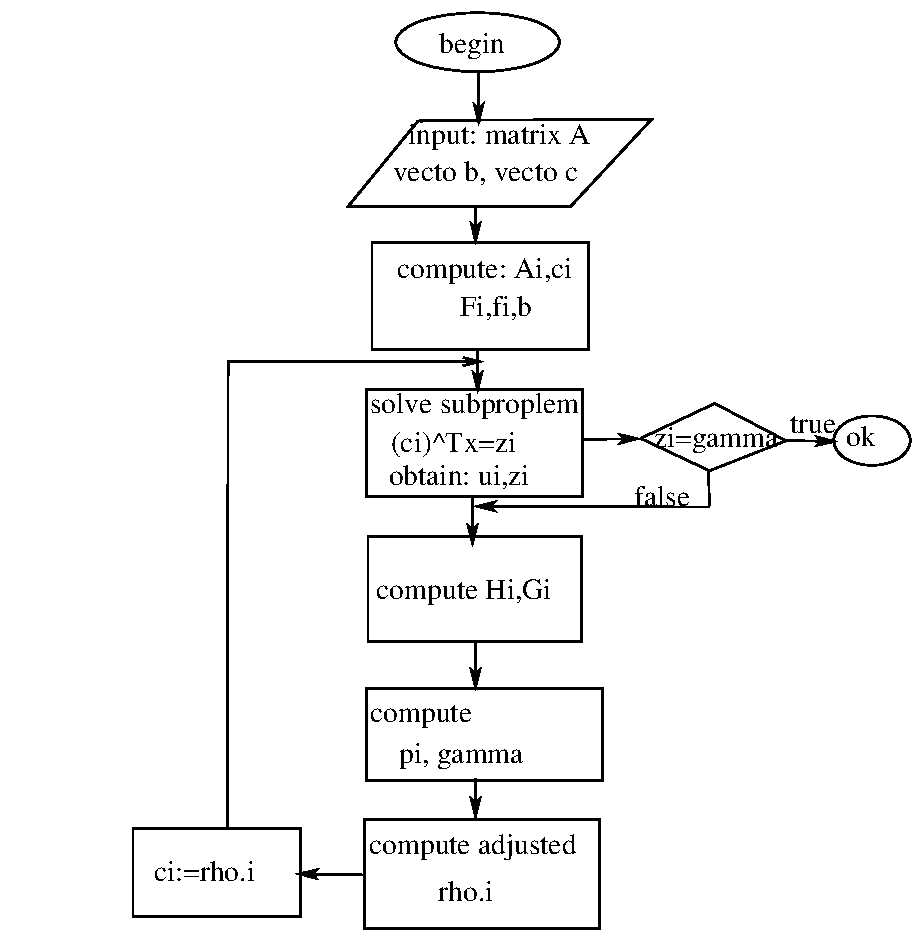
\includegraphics{sodokhoi.pdf}
\caption{sơ đồ thuật toán}\label{fig:}
\end{center}
\end{figure}

%+ 3.2.4. Triển khai xay dụng chuong trinh
\subsection{Một số thủ tục cơ bản của chương trình. }
Chương trình thể hiện phương pháp phân rã Dantzig-Wolfe có nhiều module khác nhau, được thiết kế riêng rẽ thuận tiện cho việc kiểm tra, sữa lồi, bão trì... Dưới đây là một số module cơ bản nhất:
\begin{itemize}
\item[$1.$] Private Function Doc\_m(textfile As String) As Integer 'Hàm đọc số ràng buộc từ tệp.
\item[$2.$] Private Function DocMT(textfile As String, mask As String) As String ' Hàm đọc ma trận từ tệp.
\item[$3.$] Private Function DocVT(textfile As String, mask As String) As String 'Hàm đọc vec tơ từ tệp.
\item[$4.$] Private Function phan\_ra(strA As String) As String 'Hàm phân rã ma trận A.
\item[$5.$] Private Function so\_khoi(strPR As String) As Integer 'Hàm tìm số khối xuất hiện trong ma trận A.
\item[$6.$] Private Sub GiaiBT\_DZW(textfile As String) 'Thủ tục giải bài toán D-W.
\end{itemize}

%+ Bai 3.3. Trien khai
\section{Các bước triển khai thực thi thuật toán. }
Với mục đích đưa những thuật toán có sẵn vào những ứng dụng thực tế, khóa luận này sẽ trình bày tóm tắt lại những khâu cơ bản trong quá trình triển khai thực thi một thuật toán nhằm giải quyết các bài tóan ứng dụng cụ thể. Tùy thuộc vào mục đích ứng dụng, thời gian thực hiện, chi phí, quy mô của bài toán ứng dụng, mà người ta lựa chọn những quy trình thực hiện khác nhau. Chẳng hạn dưới đây là một số bước cơ bản khi triển khai áp dụng:

\begin{itemize}
\item{\bf Bước 1. } Xây dựng mô hình định tính cho bài toán bằng cách tham biến (tham số) hoá các thành phần của bài toán thực tế. Nói cách khác là lượng hoá hoặc hình thức hoá các đối tượng thực tế bằng các ký hiệu hoặc lược đồ...Trong một số trường hợp cần phân chia, hoặc hạn chế hay rút gọn bài toán thực tế thì mới có thể mô hình hoá được dưới dạng mô hình toán học.
\item {\bf Bước 2. } Xây dựng mô hình toán học, bằng cách liên kết các đối tượng theo các mối quan hệ thành các công thức tường minh hoặc quan hệ cụ thể. Đồng thời với nó là xác định mục tiêu (một hoặc nhiều mục tiêu) cho bài toán thực tế và lượng hoá nó thành hàm mục tiêu cho bài toán tối ưu.
\item {\bf Bước 3. } Sử dụng các công cụ của toán học, cụ thể là lý thuyết tối ưu để giải quyết bài toán. Bước này cần thực hiện một cách khoa học và tuân thủ theo yêu cầu đặt ra ban đầu. Đó là phân loại bài toán, nghiên cứu các tính chất định tính, sự tồn tại nghiệm, xây dựng thuật toán giải (chương trình hoá bằng chương trình máy tính hoặc xây dựng được một lược đồ tính toán (thủ công)), đánh giá hiệu quả của phương pháp trên các phương diện: thời gian, kinh phí, phương tiện, độ chính xác, độ ổn định và tính tin cậy...
\item{\bf Bước 4. } Áp dụng vào bài toán thực tế, phân tích và kiểm định với bài toán thực tế, đánh giá kết quả và mức độ phù hợp. Có thể xảy ra hai khả năng.
\begin{enumerate}
\item Mô hình tính toán là phù hợp với thực tế. Khi đó cần tổng kết lại (thành tài liệu nghiên cứu và hướng dẫn) và có thể đưa ra áp dụng rộng rãi. Sau đó cần tính đến vấn đề kiểm định và bảo trì cũng như hướng phát triển của hệ thống trong tương lai.
\item Mô hình tính toán không phù hợp với thực tế. Khi đó cần rà soát lại các bước thực hiện để tìm ra nguyên nhân của nó. Có thể có nhiều nguyên nhân, trong đó có các nguyên nhân chủ yếu thường gặp sau: Do lựa chọn mô hình hoá toán học chưa phù hợp, công cụ giải quyết chưa phù hợp (chưa có công cụ đủ mạnh), sai số của dữ liệu (do quá trình đo đạc, quan sát, ảnh hưởng cuả môi trường...), độ chính xác và độ ổn định của thuật toán chưa được kiểm định... Do vậy cần tìm cách để khắc phục hoặc tìm hướng mới để giải lại bài toán.
\end{enumerate}
\end{itemize}
%%%%%%%%%%%%%%%%%%%%%%%%%%%%%%%%%%%%%%%%%%%


\newpage
%+ ======================================================================================================================
%+ Noi dung: PHU LUC
%+ ======================================================================================================================
\chapter*{Phụ lục}
Phụ lục này sẽ trình bày một số modules cơ bản của thuật toán đơn hình gốc của Dantzig ,và một số module của phương pháp phân rã Dantzig-Wolfe dưới dạng ngôn ngữ Visual Basic, phiên bản 6.0.

Cụ thể sẽ trình bày các thủ tục sau:\\
\noindent{\bf 1. Modul thuật toán đơn hình gốc của Dantzig}
{\footnotesize
\\noindent{\bf 1. Modul thuật toán đơn hình gốc của Dantzig}
\begin{verbatim}
Private Sub QHTT()
    'Bo xung vao ma tran A
    Dim i, j As Integer
    Dim b_temp(30) As Double
    Dim a_temp(100, 100) As Double
    For i = 0 To m - 1
        a(i + 1, 0) = b(i + 1) 'Cot 0 ma tran a
    Next
    For i = 0 To n - 1
        a(0, i + 1) = c(i + 1)
    Next
    
    'Phuong phap don hinh
    Dim toi_uu As Boolean
    toi_uu = False
    Dim var_lap As Integer
    var_lap = 0
    While toi_uu = False
        'Tinh cac uoc luong delta
        For j = 1 To n
            a(m + 1, j) = 0
            For i = 1 To m
                a(m + 1, j) = a(m + 1, j) + acb(i) * a(i, j)
            Next
            a(m + 1, j) = a(m + 1, j) - a(0, j) 
			'Dong thu m+1 trong ma tran a luu tru cac gia tri delta
        Next
        
        ' Hien thi bang don hinh
        display (var_lap * (m + 2) + 1)
        
        'Tim delta max va s
        Dim s As Integer
        s = 1
        Dim delta As Double
        delta = a(m + 1, s)
        For j = 1 To n
            If a(m + 1, j) > delta Then
                delta = a(m + 1, j)
                s = j
            End If
        Next
        'MsgBox (CStr(delta))
        
        ' Kiem tra dieu kien toi uu
        If delta > 0 Then
            toi_uu = False
        Else
            toi_uu = True
            GoTo Ketthuc
        End If
        
        'Kiem tra vo nghiem
        Dim voNo As Boolean
        voNo = False
        For j = 1 To n
            If a(m + 1, j) > 0 Then
                dem = 1
                Do While dem <= m And a(dem, j) <= 0
                    dem = dem + 1
                Loop
                If dem > m Then
                    voNo = True
                    MsgBox ("BAI TOAN VO NGHIEM")
                    Exit Sub
                Else
                    voNo = False
                End If
            End If
        Next
            
        'Tim an loai ra
        Dim r As Integer
        r = 1
        If a(r, s) < 0 Then
            r = r + 1
        End If
        For i = r To m
            If a(i, s) > 0 Then
                For j = 1 To n
                    If a(r, j) / a(r, s) > a(i, j) / a(i, s) Then
                        r = i
                    End If
                Next
            End If
        Next
        
        'Bien doi bang
        acb(r) = a(0, s)
        cb(r) = s
        Dim ars, ais As Double
        ars = a(r, s)
        'Bien doi cac phan tu con lai
        For i = 1 To m
            For j = 1 To n
                If i <> r Then
                    b_temp(i) = b(i) - (b(r) / ars) * a(i, s)
                    a_temp(i, j) = a(i, j) - (a(r, j) / ars) * a(i, s)
                Else
                    a_temp(r, j) = a(r, j) / ars
                    b_temp(r) = b(r) / ars
                End If
            Next
        Next
        
        For i = 1 To m
            For j = 1 To n
                a(i, j) = a_temp(i, j)
                a(i, 0) = b_temp(i)
                b(i) = b_temp(i)
            Next
        Next
        
Ketthuc:
    var_lap = var_lap + 1

    Wend
End Sub
\end{verbatim}
}
\noindent{\bf 2. Modul thuật toán phân rã Dantzig-Wolfe.}
{\footnotesize
\begin{verbatim}
Private Function Doc_m(textfile As String) As Integer
    Dim m As Integer
    'Doc du lieu tu tep
    Doc_m = m
End Function
-------------------------------------------------------------------------------------------------------------------------------------------------
Private Function Doc_n(textfile As String) As Integer
    Dim n As Integer
    'Doc du lieu tu tep gan vao bien n
    Doc_n = n
End Function
-------------------------------------------------------------------------------------------------------------------------------------------------
Private Function DocMT(textfile As String, mask As String) As String
    Dim strA As String
    'Doc du lieu tu tep luu cac phan tu cua mang vao StrA
    'Cac phan tu cua chuoi strA cach nhau boi dau cach
    'Cac dong cua ma tran cach nhau boi dau (,)
    DocMT = strA
End Function
-------------------------------------------------------------------------------------------------------------------------------------------------
Private Function DocVT(textfile As String, mask As String) As String
    Dim strVT As String
    'Doc du lieu tu tep
    'Luu du lieu doc duoc la mot vec to vao strVT
    'Cac phan tu cua strVT cach nhau boi dau cach
    DocVT = strVT
End Function
-------------------------------------------------------------------------------------------------------------------------------------------------
Private Function phan_ra(strA As String) As String
    Dim strPR As String
    'strPR lu tru cac diem phan ra
    'Cac diem phan ra cach nhau boi dau (,)
    'Diem dau la (0 0) va diem cuoi la (m n)
    'Moi diem la mot cap gom 2 so la chi so hang va chi so cot cua ma tran A
    'Cac phan tu cua strPR cac nhau boi dau cach
    phan_ra = strPR
End Function
-------------------------------------------------------------------------------------------------------------------------------------------------
Private Function so_khoi(strPR As String) As Integer
    'Tim so khoi phan ra
    Dim N_khoi As Integer
    'So khoi phan ra bang so diem phan ra - 2
    so_khoi = N_khoi '= so dau (,)
End Function
-------------------------------------------------------------------------------------------------------------------------------------------------
Private Sub GiaiBT_DZW(textfile As String)
    Dim m, n, k, i, j, N_khoi As Integer
    m = Doc_m(textfile)
    n = Doc_n(textfile)
    Dim A(100, 100) As Double ' khai bao ma tran A
    Dim b(100) As Double ' Khai bao vec to b
    Dim c(100) As Double ' Khai bao vecto c
    ReDim A(m, n) '
    ReDim c(n)
    ReDim b(m)
    Dim strA, strb, strc, strPR As String
    strA = DocMT(textfile, "a:=")
    strb = DocVT(textfile, "b:=")
    strc = DocVT(textfile, "c:=")
    Dim strtemp(n) As String
    strtemp = Split(strA, ",", -1, 1)
    Dim temp
    For k = 1 To UBound(strtemp)
        temp = Split(strtemp(k), " ", -1, 1)
        For i = 1 To m
            For j = 1 To n
                A(i, j) = temp(i)
            Next
        Next
    Next
    b = Split(strb, " ", -1, 1)
    c = Split(strc, " ", -1, 1)
    strPR = phan_ra(strA)
    N_khoi = so_khoi(strPR)
    'Khai bao
    Dim Ak, fk, fk, ck, bk
    For k = 1 To N_khoi
        'Tinh Ak,Fk,fk,ck,bk
    Next
    Dim u(n), v(n)
    Dim toi_uu, lap As Boolean
    toi_uu = False
    lap = False
    While toi_uu = False
        For k = 1 To N_khoi
            'Giai cac bai toan con Subk
            ' Output tinh duoc cac uk, vk
        Next
        'Chon co so xuat phat la wk la cac vec to 0
        'Tim G, H
        Dim numberOfRowAk As Integer
        For k = 1 To UBound(uk)
            For i = 1 To numberOfRowAk
                tg1 = 0
                tg2 = 0
                For j = 1 To UBound(uk)
                    tg1 = tg1 + Ak(i, j) * uk(j)
                    tg2 = tg2 + Ak(i, j) * vk(j)
                Next
                gk(i) = tg1
                Hk(i) = tg2
            Next
        Next
        'Tim gk
        For k = 1 To N_khoi
            tg = 0
            For i = 1 To UBound(wk)
                tg = tg + chuyevi(wk(i)) * uk(i)
            Next
            gk = tg
        Next
        ' Xay dung bai toan Restricted Master
        If lap = False Then
            'Giai bai toan Restricted Master (RMas)'
            If RMas = "VoNo" Then
                'Ket thuc: Ket luan bai toan goc vo nghiem
            Else
                'Tinh pi va gamma
            End If
        Else
            'Chen Gk va Hk moi vao bai toan RMas ta duoc bai toan NewRMas
            'Giai bai toan NewRMas
            If NewRMas = "VoNo" Then
                'Ket thuc: Ket luan bai toan toan goc vo nghiem
            Else
                'Tinh pi va gamma
            End If
        End If
        ' Tinh rho
        For k = 1 To N_khoi
            For i = 1 To UBound(wk)
                tg = 0
                For j = 1 To UBound(pi)
                    tg = tg - chuyenvi(Ak(i, j)) * pi
                Next
                rhok(i) = tg + wk(i)
            Next
        Next
        'Gan c = rho
        For k = 1 To N_khoi
            For i = 1 To UBound(ck)
                ck(i) = rhok(i)
            Next
        Next
        For k = 1 To N_khoi
            'Giai bai toan Subk
            'Output: uk va zk
        Next
        'Kiem tra dieu kien toi uu
        For k = 1 To N_khoi
            If z(k) < gamma(k) Then
                ' Tinh lai Gk, Hk
                dem = dem + 1
                lap = True
            End If
        Next
        If dem = 0 Then
            toi_uu = True
            ' Ket luan phuong an toi uu cua bai toan goc
        End If
    Loop
End Sub
-------------------------------------------------------------------------------------------------------------------------------------------------
\end{verbatim}
}

\textbf{Kiểm thử kết quả ví dụ trình bày ở chương 2 bằng thuật toán đơn hình}
\textbf{Input}
\begin{verbatim}
m := 13
n := 14
c[i] := 1 2 3 4 5 6 1 2 3 4 5 6 7 -10
b[i] := 64 63 3 4 2 1 4 4 5 3 3 3 1
a[i,j] := 3 2 1 6 5 4 8 5 7 3 4 1 1 2
a[i,j] := 1 8 3 7 1 4 5 2 5 3 2 6 3 4
a[i,j] := 1 1 1 0 0 0 0 0 0 0 0 0 0 0
a[i,j] := 0 0 0 1 1 1 0 0 0 0 0 0 0 0
a[i,j] := 1 0 0 1 0 0 0 0 0 0 0 0 0 0
a[i,j] := 0 1 0 0 1 0 0 0 0 0 0 0 0 0
a[i,j] := 0 0 1 0 0 1 0 0 0 0 0 0 0 0
a[i,j] := 0 0 0 0 0 0 1 1 1 0 0 0 0 0
a[i,j] := 0 0 0 0 0 0 0 0 0 1 1 1 0 0
a[i,j] := 0 0 0 0 0 0 1 0 0 1 0 0 0 0
a[i,j] := 0 0 0 0 0 0 0 1 0 0 1 0 0 0
a[i,j] := 0 0 0 0 0 0 0 0 1 0 0 1 0 0
a[i,j] := 0 0 0 0 0 0 0 0 0 0 0 0 1 -1
\end{verbatim}
Ta có một số bước lặp minh họa bằng bảng đơn hình như sau. Tại bước lặp thứ 15 bài toán đã đạt giá trị tối ưu khi tất cả các biến giả bằng 0 và giá trị tối ưu đạt được là $f(x)=68$ ta cũng được kết quả này khi giải với thuật toán Dantzig-Wolfe trong ví dụ minh họa ở chương 2.
\begin{figure}[!ht]
\begin{center}
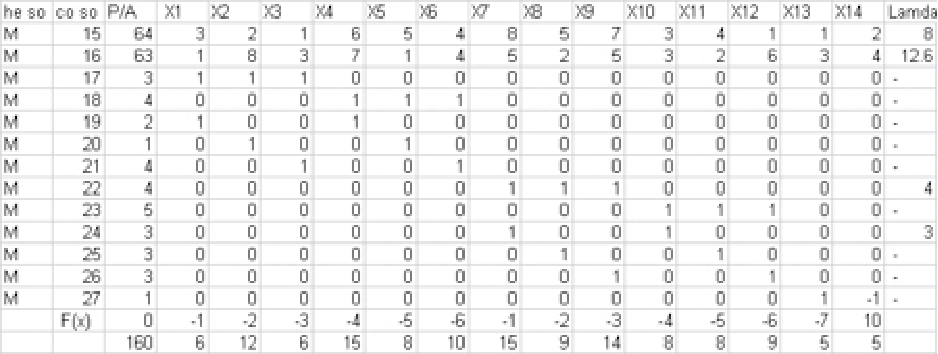
\includegraphics{lap1.pdf}
\caption{Bảng đơn hình ở bước lặp thứ 1}
\end{center}
\end{figure}
\begin{verbatim}

\end{verbatim}
\begin{figure}[!ht]
\begin{center}
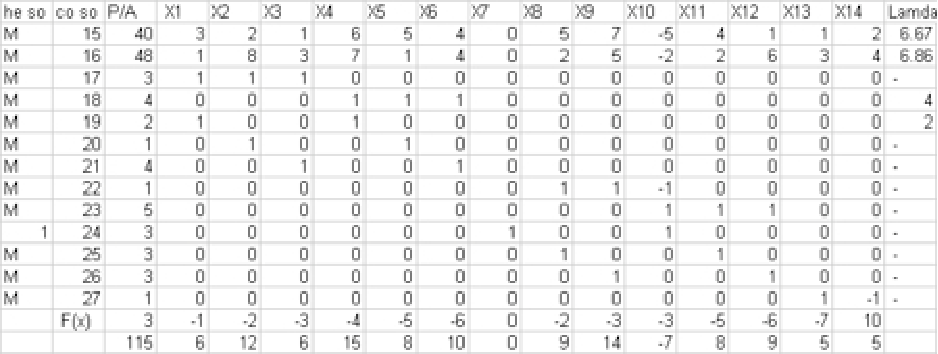
\includegraphics{lap2.pdf}
\caption{Bảng đơn hình tại bước lặp thứ 2}
\end{center}
\end{figure}
\begin{verbatim}







\end{verbatim}
\begin{figure}[!ht]
\begin{center}
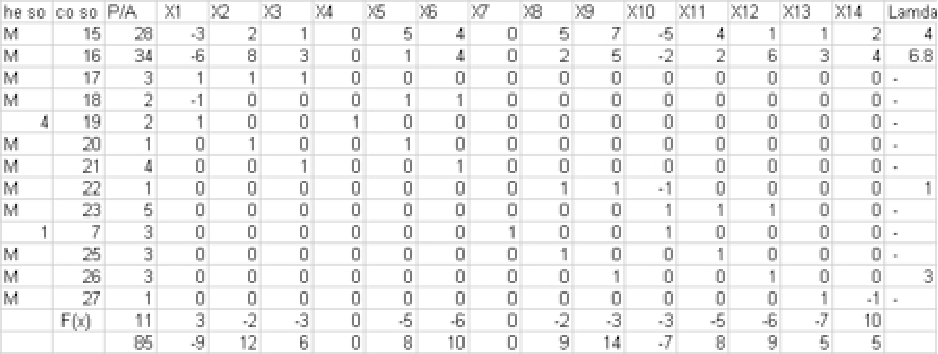
\includegraphics{lap3.pdf}
\caption{Bảng đơn hình ở bước lặp thứ 3}
\end{center}
\end{figure}

\begin{figure}[!ht]
\begin{center}
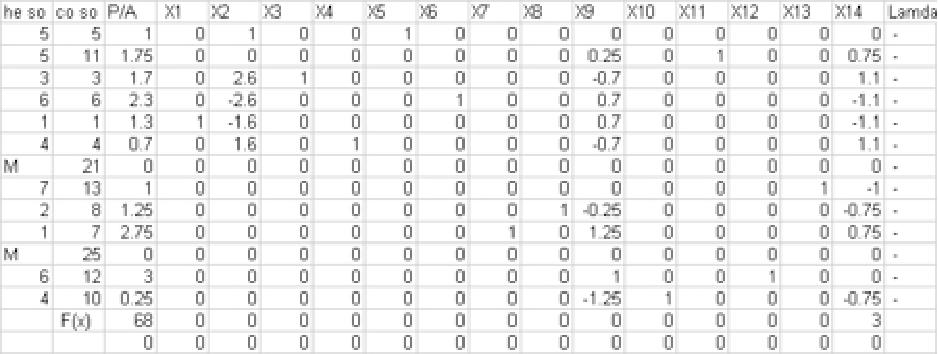
\includegraphics{lap15.pdf}
\caption{bảng đơn hình ở bước lặp thứ 15}
\end{center}
\end{figure}
\begin{verbatim}













\end{verbatim}
%+ KET THUC PHAN PHU LUC.
%+ ======================================================================================================================

%\newpage
%+ ======================================================================================================================
%+ Noi dung: KET LUAN
%+ ======================================================================================================================
\centerline{\bf \large\MakeUppercase{Kết luận}}
\vspace{20pt}

%+ --------------------------------------------------------------------------------------------------------------------------------------------------------------------------------------------------------------------
%+ Noi dung se go vao day. (Trinh bay cac ket qua chinh dat duoc, dong gop cua tac gi�, cac huong va cong viec trong tuong lai).
\normalsize{
Trong khóa luận này em đã trình bày tư tưởng nội dung, trường hợp áp dụng cho thuật toán phân rã Dantzig-Wolfe và một số thuật toán là đơn hình đơn hình đối ngẫu để phục vụ mục đích giải bài toán quy hoạch kích thước lớn. Song song là ví dụ bằng số minh họa cho phương pháp cuối cùng là lập trình với thuật toán đơn hình đơn hình bằng ngôn ngữ VB phục vụ ở một số bước của thuật toán.
Đóng góp chính của khóa luận bao gồm:

\begin{itemize}
\item[1] Tìm hiểu và trình bày lại nội dung phương pháp Dantzig-Wolfe.
\item[2] Đề cập phân tích một số dạng bài toán có kích thước lớn trong thực tế áp dụng phương pháp Dantzig-Wole.
\item[3] Lập trình với thuật toán đơn hình để phục vụ một số bước của thuật toán ngoài ra còn có tác dụng kiểm thử với các bài toán nhỏ.
\end{itemize}
Tuy nhiên do thời gian thực hiện khóa luận không nhiều còn có những sai sót em rất mong nhận được sự góp ý của quý thầy cô và bạn đọc.}



%+ --------------------------------------------------------------------------------------------------------------------------------------------------------------------------------------------------------------------


%+ ======================================================================================================================
%+ KET THUC PHAN KET LUAN.
%+ ======================================================================================================================



\newpage
%+ ======================================================================================================================
%+ Noi dung: TAI LIEU THAM KHAO
%+ ======================================================================================================================
\begin{thebibliography}{50}
%+ --------------------------------------------------------------------------------------------------------------------------------------------------------------------------------------------------------------------
%+ Noi dung : Trinh bay cac tai lieu tham khao theo thu tu A->Z
%+ --------------------------------------------------------------------------------------------------------------------------------------------------------------------------------------------------------------------
%\normalsize{
\bibitem{[Kha]} Phan Quốc Khánh  - Trần Huệ Nương, {\it Quy hoạch tuyến tính}, NXB Giáo dục (2000) 457 trang.

\bibitem{[Tha]} Nguyễn Ngọc Thắng - Nguyễn Đình Hóa, {\it Quy hoạch tuyến tính}, NXB Đại học Quốc Gia Hà Nội (2006) 148 trang.

\bibitem{[Dan]}Danzig G.B and Thapa M.N, {\it Linear programming 2 - Theory and Extensions},Springer Verlag, New York Berlin, Heideiberg,(2003)

\bibitem{[Jor]}Jorge Nocedal Stephen J.Wright, {\it Numerical Optimization}, Springer (2006).

\bibitem{[Jor]}Trần Tuấn, {\it Đồ án hay}, NXB Bách khoa (2006).
%+ -------------------------------------------------------------------------------------------------------------------------------------------------------------------------------------------------------------------
\end{thebibliography} 
%+ ======================================================================================================================
%+ KET THUC PHAN PHU LUC.
%+ ======================================================================================================================


\end{document}
